%---------------------------------------------------------------------
%  Writeup of the latest and  greatest search of Run II data for
%  single top quark production at DZero.
%  Started 08/31/06
%  Continued 10/14/06
%  Authors: The Single Top Working Group
%
%---------------------------------------------------------------------
%
\documentclass[aps]{revtex4}

% Allow figures to be included
\usepackage{graphicx}

% Allow type to be colored (68 colors)
\usepackage[usenames]{color}

% Allow rotation of tables, figures, pages
\usepackage{rotating}

% Add a gray bar to the margin for new text
\usepackage{changebar}

% Allow sub figures
\usepackage{subfigure}

% Fix too narrow margins
\paperheight 11 in
\paperwidth 8.5 in
\textwidth 6.5 in
\oddsidemargin 0 pt
\marginparsep 0 pt
\marginparwidth 0 pt
\voffset 0 in
\hoffset 0 in

% Fix hard-to-follow section numbering
\renewcommand{\thesection}
{\Large\arabic{section}}
\renewcommand{\thesubsection}
{\large\arabic{section}.\large\arabic{subsection}}
\renewcommand{\thesubsubsection}
{\arabic{section}.\arabic{subsection}.\arabic{subsubsection}}
\renewcommand{\theparagraph}
{\arabic{section}.\arabic{subsection}.\arabic{subsubsection}.\arabic{paragraph}}

% Change the table numbering from roman to arabic
\renewcommand{\thetable}{\arabic{table}}

% Fix problems with font changes after a reference to a section 
\let\LaTEXref\ref
\renewcommand{\ref}[1]
{{\LaTEXref{#1}}}

% Make section titles size match text size
\makeatletter
\renewcommand{\section}{\@startsection
	{section}%
	{1}%
	{0pt}%
	{-\baselineskip}%
	{1.0\baselineskip}%
	{\center\bfseries\Large\rmfamily\scshape}}%
\renewcommand{\subsection}{\@startsection
	{subsection}%
	{2}%
	{0pt}%
	{-\baselineskip}%
	{1.0\baselineskip}%
	{\center\bfseries\large\rmfamily}}%
\renewcommand{\subsubsection}{\@startsection
	{subsubsection}%
	{3}%
	{0pt}%
	{-\baselineskip}%
	{1.0\baselineskip}%
	{\center\itshape\large\rmfamily}}%
\renewcommand{\paragraph}{\@startsection
	{paragraph}%
	{4}%
	{0pt}%
	{-\baselineskip}%
	{1.0\baselineskip}%
	{\center\itshape\rmfamily}}%

% Fix references to sections
\renewcommand{\p@subsection}{}
\renewcommand{\p@subsubsection}{}
\renewcommand{\p@paragraph}{}
\renewcommand{\p@subparagraph}{}

\makeatother

% Put page number at bottom of page
\pagestyle{plain}

% Avoid too much hyphenation at the ends of lines
\lefthyphenmin=6
\righthyphenmin=6

% Allow a figure to occupy most of a column without being
% placed on a separate page that includes no text
\renewcommand{\topfraction}      {0.95}
\renewcommand{\bottomfraction}   {0.95}
\renewcommand{\floatpagefraction}{0.95}
\renewcommand{\textfraction}     {0.05}

% Tighten up the itemized lists
\newenvironment{myitemize}{\begin{itemize}
                \setlength{\itemsep}{-1 pt}}{\end{itemize}}

% Define some abbreviations
\newcommand{\dzero}     {D\O}
\newcommand{\met}       {\mbox{$\not\!\!E_T$}}
\newcommand{\pt}        {\mbox{$p_{\rm T}$}}
\newcommand{\deta}      {\mbox{$\eta^{\rm det}$}}
\newcommand{\meta}      {\mbox{$\left|\eta\right|$}}
\newcommand{\mdeta}     {\mbox{$\left|\eta^{\rm det}\right|$}}
\newcommand{\rar}       {\rightarrow}
\newcommand{\rargap}    {\mbox{ $\rightarrow$ }}
\newcommand{\tbbar}     {\mbox{$tb$}}
\newcommand{\tqbbar}    {\mbox{$tqb$}}
\newcommand{\ttbar}     {\mbox{$t\bar{t}$}}
\newcommand{\bbbar}     {\mbox{$b\bar{b}$}}
\newcommand{\ccbar}     {\mbox{$c\bar{c}$}}
\newcommand{\qqbar}     {\mbox{$q\bar{q}$}}
\newcommand{\ppbar}     {\mbox{$p\bar{p}$}}
\newcommand{\lepjets}   {\mbox{$t\bar{t} \rightarrow \ell$+jets}}
\newcommand{\dilepton}  {\mbox{$t\bar{t} \rightarrow \ell$+$\ell$}}
\newcommand{\comphep}   {\sc{c}\rm{omp}\sc{hep}}
\newcommand{\singletop} {\sc{s}\rm{ingle}\sc{t}\rm{op}}
\newcommand{\herwig}    {\sc{herwig}}
\newcommand{\pythia}    {\sc{pythia}}
\newcommand{\alpgen}    {\sc{alpgen}}
\newcommand{\tauola}    {\sc{tauola}}
\newcommand{\evtgen}    {\sc{e}\rm{vt}\sc{g}\rm{en}}
\newcommand{\reco}      {\sc{reco}}
\newcommand{\pderiv}[2]{\frac{\partial #1}{\partial #2}}
%---------------------------------------------------------------------
%---------------------------------------------------------------------
\begin{document}

\begin{table}
\begin{flushleft}
\begin{minipage}{5.5 in}
\begin{tabular}{lr}
{\leftline{\includegraphics[scale=0.3]{figures/d0logo}}}
& \hspace{-0.5in}{\large{\dzero} Note 5285} \\
%{\large For Top Group and EB review}
& \hspace{-0.5in}{\large November 28, 2006} \\
%{\large Comments to d0-run2eb-024@fnal.gov,}
& \hspace{-0.5in}{\large Version 1.3} \\
%{\large Ar\'{a}n~Garc\'{\i}a-Bellido, and Ann~Heinson} & \\
%{\large {\color{red}{Deadline: Friday, November 10, 2006}}} & \\
\end{tabular}
\end{minipage}
\end{flushleft}
\end{table}

\title{\LARGE{Search for Single Top Quark Production\\
in 1~fb$^{-1}$ of Data}\\
\vspace{0 in}}

%--------
%  Secret title is something like ``New Mode of Top Quark Production
%  Observed at the Tevatron''
%--------

\author{\large{
E.~Aguil\'{o},$^{2}$
P.~Baringer$^{10}$
A.~Bean,$^{10}$
C.~Belanger-Champagne,$^{11}$
J.A.~Benitez,$^{12}$
E.E.~Boos,$^{13}$
R.~Brock,$^{12}$
V.~Bunichev, $^{13}$
K.~Chan,$^{2}$
L.~Christofek,$^{4}$
Y.~Coadou,$^{17}$
L.V.~Dudko,$^{13}$
M.~Erdmann,$^{1}$
T.~Gadfort,$^{18}$
A.~Garc\'{\i}a-Bellido,$^{18}$
C.~Gerber,$^{9}$
D.~Gillberg,$^{17}$
G.~Gutierrez,$^{7}$
P.~Gutierrez,$^{14}$
A.P.~Heinson,$^{5}$
U.~Heintz,$^{3}$
S.~Herrin,$^{16}$
S.~Jabeen,$^{3}$
S.~Jain,$^{14}$
A.~Juste,$^{7}$
S.~Kappler,$^{1}$
D.~Kau,$^{8}$
G.~Kertzscher,$^{11}$
M.~Kirsch,$^{1}$
L.~Li,$^{5}$
J.~Mitrevski,$^{6}$
R.~Moore,$^{2}$
M.~Narain,$^{3,4}$
D.~O'Neil,$^{17}$
M.~Pangilinan,$^{3}$
J.~Parsons,$^{6}$
M.~Perfilov,$^{13}$
C.~Potter,$^{11}$
H.B.~Prosper,$^{8}$
R.~Schwienhorst,$^{12}$
E.~Shabalina,$^{9}$
J.~Steggemann,$^{1}$
T.~Tim,$^{9}$
C.~Tully,$^{15}$
M.~Vetterli,$^{17}$
B.~Vachon,$^{11}$
G.~Watts,$^{18}$
M.~Weber$^{7}$
}}

\affiliation{\large{\vspace*{0.1in}
$^{1}$RWTH Aachen University\\
$^{2}$University of Alberta\\
$^{3}$Boston University\\
$^{4}$Brown University\\
$^{5}$University of California, Riverside\\
$^{6}$Columbia University\\
$^{7}$Fermi National Accelerator Laboratory\\
$^{8}$Florida State University\\
$^{9}$University of Illinois, Chicago\\
$^{10}$University of Kansas\\
$^{11}$McGill University\\
$^{12}$Michigan State University\\
$^{13}$Moscow State University\\
$^{14}$University of Oklahoma\\
$^{15}$Princeton University\\
$^{16}$Rice University\\
$^{17}$Simon Fraser University\\
$^{18}$University of Washington
}}

\begin{abstract}
{\large{We present the results of a search for single top quark
production in nearly 1~fb$^{-1}$ of Run II data. We select
single-top-like data events and separate them from backgrounds using
three different analysis methods. We use the signal acceptance,
background, and observed data in each discriminant output bin to
measure the single top quark cross section:
$$
\begin{array}{lll}
\sigma\left({\ppbar}{\rargap}tb+tqb+X\right)
& = 4.9 ^{+1.4}_{-1.4}~{\rm pb} & {\rm (Decision~trees)}\\
& = 4.6 ^{+1.8}_{-1.5}~{\rm pb} & {\rm (Matrix~elements)}\\
& = 5.0 ^{+1.9}_{-1.9}~{\rm pb} & {\rm (Bayesian~neural~networks)}
\end{array}
$$
The probability for the background to have fluctuated up to give at
least the cross section measured in the decision tree analysis is
$0.033\%$, which corresponds to a Gaussian equivalent significance of
$3.4\sigma$.
}}

\end{abstract}

\maketitle

%---------------------------------------------------------------------
%---------------------------------------------------------------------
%---------------------------------------------------------------------
%---------------------------------------------------------------------
%\clearpage
\tableofcontents
\vfill\eject

\large{

%---------------------------------------------------------------------
%---------------------------------------------------------------------
% Overview of single top and the analysis and description of changes
% with respect to the previous one
\clearpage
\input{introductionF06}

%---------------------------------------------------------------------
%---------------------------------------------------------------------
% Descriptions of the data and MC samples, integrated lumis, triggers?
% and sample sizes
\clearpage
\input{initialsamplesF06}

%---------------------------------------------------------------------
%---------------------------------------------------------------------
% Object ID
\clearpage
\input{objectidentificationF06}

%---------------------------------------------------------------------
%---------------------------------------------------------------------
% Selection cuts
\clearpage
%---------------------------------------------------------------------
%  Writeup of the improved search of Run II data for single top quark
%  production at DZero.
%  Started: Oct 2006
%  Authors: The Single Top Working Group
%---------------------------------------------------------------------
%

\section{Event Selection Cuts}
\label{selection-cuts}

We apply a loose event selection to find $W$-like events containing an
isolated lepton, missing transverse energy, and one to four jets with
high transverse momentum. The samples after this selection, which we
call ``pretagged,'' are dominated by $W$+jets events, with some
{\ttbar} contribution which becomes more significant for higher jet
multiplicities. To be able to extract single top events we also look
for the presence of one or two $b$-tagged jets.

Common selection for both electron and muon channels:
\vspace{-0.08in}
\begin{myitemize}
\item Good quality~\cite{dataquality} (for data)
\item Pass trigger: offline electrons and muons in the data are
matched to the object that fired the appropriate trigger for that
run period and triggerlist
\item Good primary vertex: $|z_{\rm PV}| < 60$~cm with at least three
tracks attached
\item Missing transverse energy $15 < {\met} < 200$~GeV
\item One, two, three or four jets with ${\pt} > 15$~GeV and
$|\deta|<3.4$ 
\item The leading jet is required to have ${\pt} > 25$~GeV and
$|\deta| < 2.5$
\item The second leading jet is required to have ${\pt} > 20$~GeV
\item There must be fewer than three noise jets
\item Jet triangle cut $|\Delta\phi({\rm leading~jet,{\met}})|
{\rm ~vs.~}{\met}$: from 1.5 to $\pi$~radians when ${\met} = 0$~GeV,
and {\met} from 0 to 35~GeV when $|\Delta\phi| = \pi$~rad
\end{myitemize}

\vspace{-0.07in}
The electron channel selection: 
\vspace{-0.07in}
\begin{myitemize}
\item Only one tight electron with $E_T > 15$~GeV and
$|\deta| < 1.1$
\item No second loose electron with $E_T > 15$~GeV
\item No tight muon with ${\pt} > 18$~GeV and $|\deta| < 2.0$ 
\item Electron coming from the primary vertex:
$|\Delta z(e,{\rm PV})| < 1$~cm
\item Electron triangle cuts $|\Delta\phi({\rm e,{\met}})|{\rm ~vs.~}
{\met}$:
   \vspace{-0.07in} 
   \begin{myitemize}
   \item from 2 to 0~rad when ${\met} = 0$~GeV, and {\met} from 0
   to 40~GeV when $|\Delta\phi| = 0$~rad
   \item from 1.5 to 0~rad when ${\met} = 0$~GeV, and {\met} from 0
   to 50~GeV when $|\Delta\phi| = 0$~rad
   \item  from 2 to $\pi$~rad when ${\met} = 0$~GeV, and {\met}
   from 0 to 24~GeV when $|\Delta\phi| = \pi$~rad
   \end{myitemize}
\end{myitemize}

\vspace{-0.07in}
The muon channel selection: 
\vspace{-0.07in}
\begin{myitemize}
\item Only one tight muon with ${\pt} > 18$~GeV and $|\deta| < 2.0$ 
\item No tight electron with ${\pt} > 15$~GeV and within $|\deta|
< 2.5$
\item Muon coming from the primary vertex: $|\Delta z(\mu,{\rm PV})|
< 1$~cm
\item Muon triangle cuts $|\Delta\phi(\mu,{\rm {\met}})|{\rm ~vs.~}
{\met}$: 
   \vspace{-0.07in}
   \begin{myitemize}
   \item  from 1.1 to 0~rad when ${\met} = 0$~GeV, and {\met}
   from 0 to 80~GeV when $|\Delta\phi| = 0$~rad
   \item  from 1.5 to 0~rad when ${\met} = 0$~GeV, and {\met}
   from 0 to 50~GeV when $|\Delta\phi| = 0$~rad
   \item from 2.5 to $\pi$~rad when ${\met} = 0$~GeV, and {\met}
   from 0 to 30~GeV when $|\Delta\phi| = \pi$~rad
   \end{myitemize}
\end{myitemize}

\vspace{-0.07in}
Orthogonal samples selection (for measuring the multijet backgrounds):
\vspace{-0.07in}
\begin{myitemize}
\item All the same selection cuts as listed above except for the
tight lepton requirements
\item Electron channel --- only one loose-but-not-tight electron
\item Muon channel --- only one loose-but-not-tight muon
\end{myitemize}
\vspace{-0.07in}
The definitions of loose and tight electrons and muons are given in
Sections~\ref{electron-id} and \ref{muon-id}.

\noindent We also select two cross-check samples, see Appendix~6 for
details.





%---------------------------------------------------------------------
%---------------------------------------------------------------------
% Event numbers
\clearpage
%---------------------------------------------------------------------
%  Writeup of the improved search of Run II data for single top quark
%  production at DZero.
%  Started: Oct 2006
%  Authors: The Single Top Working Group
%---------------------------------------------------------------------
%
\section{Numbers of Events After Selection}
\label{event-numbers}

Table~\ref{numbers-of-events} shows the numbers of events in the
signal and background samples and in the data after applying the
selection criteria shown in Section~\ref{selection-cuts}. (Note, the
numbers of events shown in this Table are not the yields, which are
shown later in Section~\ref{event-yields}.) The numbers of events are
important when training a discriminant on them, or when calculating
statistical uncertainties on the backgrounds and signals.

\begin{table}[!h!tbp]
\begin{center}
\begin{minipage}{6.5 in}
\begin{ruledtabular}
\begin{tabular}{l||ccccc|ccccc}
\multicolumn{11}{c}{\hspace{1in}\underline{Numbers of Events after Selection}} \vspace{0.1in}\\
& \multicolumn{5}{c|}{Electron Channel} & \multicolumn{5}{c}{Muon Channel} \\
                         & 1 jet & 2 jets & 3 jets & 4 jets & 5+ jets
                         & 1 jet & 2 jets & 3 jets & 4 jets & 5 jets \\
\hline			                   
Signal MC                &         &        &        &        &        &         &        &        &        &       \\
~~$tb$                   &   6,908 & 19,465 &  9,127 &  2,483 &   595  &   3,878 & 12,852 &  6,458 &  1,809 &   401 \\
~~$tqb$                  &   8,971 & 22,758 & 12,080 &  3,797 &  1,092 &   8,195 & 21,066 & 11,193 &  3,489 &   835 \\
~~$tb$+$tqb$             &  15,879 & 42,223 & 21,207 &  6,280 &  1,687 &  12,073 & 33,918 & 17,651 &  5,298 & 1,236 \\
Background MC            &         &        &        &        &        &         &        &        &        &       \\
~~${\ttbar}{\rar}ll$	 &   7,671 & 29,537 & 26,042 & 12,068 &  5,396 &   5,509 & 24,595 & 21,803 &  9,788 & 3,442 \\
~~${\ttbar}{\rar}l$+jets &     522 &  5,659 & 22,477 & 27,319 & 14,298 &     232 &  3,376 & 16,293 & 22,680 & 8,658 \\ 
~~$Wb\bar{b}$            &  26,611 & 13,914 &  9,011 &  3,848 &  1,434 &  27,764 & 14,488 &  9,427 &  3,874 & 1,204 \\
~~$Wc\bar{c}$            &  21,765 & 13,453 &  7,562 &  2,252 &    591 &  32,712 & 19,047 & 10,141 &  3,051 &   663 \\
~~$Wjj$                  & 134,660 & 61,497 & 34,162 &  8,290 &  1,750 & 147,842 & 66,201 & 36,673 &  9,169 & 1,502 \\
Pretag data              &         &        &        &        &        &         &        &        &        &       \\
~~Multijets              &  11,565 &  6,993 &  4,043 &  1,317 &    431 &     897 &    658 &    462 &    151 &    48 \\
~~Signal data            &  27,370 &  8,220 &  3,075 &    874 &    223 &  17,816 &  6,432 &  2,590 &    727 &   173 \\
ZeroTag data             &         &        &        &        &        &         &        &        &        &       \\
~~Multijets              &  11,319 &  6,659 &  3,802 &  1,210 &    390 &     866 &    604 &    409 &    128 &    36 \\
~~Data                   &  26,925 &  7,833 &  2,831 &    752 &    178 &  17,527 &  6,122 &  2,378 &    599 &   125 \\
OneTag data              &         &        &        &        &        &         &        &        &        &       \\
~~Multijets              &     246 &    322 &    226 &     93 &     34 &      31 &     51 &     49 &     21 &     8 \\
~~Signal data            &     445 &    357 &    207 &     97 &     35 &     289 &    287 &    179 &    100 &    38 \\
TwoTags data             &         &        &        &        &        &         &        &        &        &       \\
~~Multijets              &     --- &     12 &     15 &     14 &      7 &     --- &      3 &      4 &      1 &     4 \\
~~Signal data            &     --- &     30 &     37 &     22 &     10 &     --- &     23 &     32 &     27 &    10 
\end{tabular}
\end{ruledtabular} 
\vspace{-0.1in}
\caption[numbersofevents]{Numbers of events for the electron and muon
channels after selection.}
\label{numbers-of-events}
\end{minipage}
\end{center}
\end{table}





%---------------------------------------------------------------------
%---------------------------------------------------------------------
% How we measure the backgrounds
\clearpage
\input{backgroundmethodsF06}

%---------------------------------------------------------------------
%---------------------------------------------------------------------
% Signal acceptances
\clearpage
%---------------------------------------------------------------------
%  Writeup of the improved search of Run II data for single top quark
%  production at DZero.
%  Started: Oct 2006
%  Authors: The Single Top Working Group
%---------------------------------------------------------------------
%
\section{Signal Acceptances}
\label{signal-acceptances}

The signal acceptance is defined as:
$$
\cal{A} = \frac{\cal{B}}{N_{\rm initial}}
\displaystyle \sum_{N_{\rm selected}} \varepsilon_{\rm trigger}
\varepsilon_{\rm corrections} \varepsilon_{\rm TRF}
$$
\noindent where $\cal{B}$ is the branching fraction for the MC
sample, see Table~\ref{mcstats}, $N_{\rm initial}$ is the initial
number of events in each MC sample (also shown in
Table~\ref{mcstats}), $N_{\rm selected}$ is the number of MC events
remaining after selection, and the $\varepsilon$'s are efficiency
correction factors to account for differences between data and MC from
the trigger, particle ID, the $b$-tagging tag-rate functions, and so
forth (see Section~\ref{mc-modeling}).

Table~\ref{acceptances} shows the percentage of each single top quark
signal that remain after selection, and after $b$-tagged jets have
been required. We can compare the acceptances obtained in this
analysis with the published one~\cite{run2-d0-plb}. In that analysis,
we kept 2.6\% of the s-channel events before tagging (with 2--4 jets)
in the electron channel and 2.5\% in the muon channel. In this
analysis, we keep 2.8\% and 2.2\% in the electron and muon channels
respectively (2--4 jets). In the t-channel, in the published analysis
we kept 2.6\% and 2.4\% in the electron and muon channels, and now we
are keeping 2.5\% and 2.0\%. After $b$~tagging, before we kept 1.3\%
of the electron events and 1.3\% of the muon events in the s-channel;
we now keep 1.8\% and 1.4\% respectively. In the t-channel after
$b$~tagging, we kept before 0.9\% in each of the electron and muon
channels. We now keep 1.2\% and 0.9\% of these tagged events.  The
higher acceptances now are from the use of the more efficient neural
network $b$-tagging algorithm, and probably also from the lower
reconstruction threshold for jets.

% The following is commented out until the comparison is updated to
% be for their latest results.
%
%We can also compare these acceptances to those obtained by CDF in
%their most recent analysis. For s-channel and t-channel combined,
%electron and muon channels combined, and events with exactly two jets
%with one or both $b$~tagged, they keep 1.4\% of the expected
%signal. For the same requirements, we also keep 1.4\% of the expected
%signal. In addition we have available to analyze the acceptances in
%the 1, 3, and 4-jets channels, and the untagged 2, 3, and 4-jets
%channels, which CDF have not yet included in their results.

\vspace{0.2in}
\begin{table}[!h!tbp]
\begin{center}
\begin{minipage}{6.5in}
\begin{ruledtabular}
\begin{tabular}{l||ccccc|ccccc}
\multicolumn{11}{c}{\hspace{1in}\underline{Signal Acceptances}}\vspace{0.1in} \\
& \multicolumn{5}{c|}{Electron Channel} & \multicolumn{5}{c}{Muon Channel} \\
                     & 1 jet & 2 jets & 3 jets & 4 jets & 5+ jets
                     & 1 jet & 2 jets & 3 jets & 4 jets & 5 jets \\
\hline
Before $b$ tagging   &        &        &        &        &        &        &        &        &        &        \\
~~$tb$               & 0.55\% & 1.77\% & 0.83\% & 0.23\% & 0.06\% & 0.33\% & 1.36\% & 0.69\% & 0.19\% & 0.05\% \\
~~$tqb$              & 0.52\% & 1.49\% & 0.79\% & 0.25\% & 0.07\% & 0.36\% & 1.17\% & 0.64\% & 0.20\% & 0.05\% \\
Zero $b$-tagged jets &        &        &        &        &        &        &        &        &        &        \\
~~$tb$               & 0.32\% & 0.65\% & 0.31\% & 0.09\% & 0.02\% & 0.18\% & 0.48\% & 0.25\% & 0.07\% & 0.02\% \\
~~$tqb$              & 0.34\% & 0.86\% & 0.41\% & 0.12\% & 0.03\% & 0.23\% & 0.66\% & 0.32\% & 0.09\% & 0.02\% \\
One $b$-tagged jet   &        &        &        &        &        &        &        &        &        &        \\
~~$tb$               & 0.24\% & 0.82\% & 0.39\% & 0.11\% & 0.03\% & 0.15\% & 0.64\% & 0.32\% & 0.09\% & 0.02\% \\
~~$tqb$              & 0.18\% & 0.61\% & 0.34\% & 0.11\% & 0.03\% & 0.13\% & 0.50\% & 0.28\% & 0.09\% & 0.02\% \\
Two $b$-tagged jets  &        &        &        &        &        &        &        &        &        &        \\
~~$tb$               &  ---   & 0.29\% & 0.14\% & 0.04\% & 0.02\% &  ---   & 0.24\% & 0.12\% & 0.03\% & 0.01\% \\
~~$tqb$              &  ---   & 0.02\% & 0.05\% & 0.02\% & 0.01\% &  ---   & 0.01\% & 0.04\% & 0.02\% & 0.01\%
\end{tabular}
\end{ruledtabular}
\vspace{-0.1in}
\caption[acceptances]{Acceptances after selection.}
\label{acceptances}
\end{minipage}
\end{center}
\end{table}



%---------------------------------------------------------------------
%---------------------------------------------------------------------
% Event yields
\clearpage
%---------------------------------------------------------------------
%  Writeup of the improved search of Run II data for single top quark
%  production at DZero.
%  Started: Oct 2006
%  Authors: The Single Top Working Group
%---------------------------------------------------------------------
%
\section{Event Yields}
\label{event-yields}

We use the term ``yield'' to mean the number of events of the signal
or background in question predicted to be in the nearly 1~fb$^{-1}$ of
data analyzed here. Tables~\ref{pretag-yields}, \ref{zerotag-yields},
\ref{onetag-yields}, and \ref{twotag-yields} show these yields for all
signals and backgrounds separated by lepton flavor and jet
multiplicity within each table, and by the numbers of $b$-tagged jets
between the tables. Because the $W$+jets and multijet backgrounds are
normalized to data before tagging, the sum of the backgrounds is
defined to equal the number of events observed in the data, as seen in
the first table. Note also that the yield values shown in these tables
have been rounded to integers for clarity, so that the sums of the
components will not always equal exactly the values given for these
sums. All calculations however have been done with full-precision
values.

\begin{table}[!h!tbp]
\begin{center}
\begin{minipage}{6in}
\begin{ruledtabular}
\begin{tabular}{l||ccccc|ccccc}
\multicolumn{11}{c}{\hspace{1in}\underline{Yields Before $b$-Tagging}} \vspace{0.1in} \\
& \multicolumn{5}{c|}{Electron Channel} & \multicolumn{5}{c}{Muon Channel} \\
                         & 1 jet & 2 jets & 3 jets & 4 jets & 5+ jets
                         & 1 jet & 2 jets & 3 jets & 4 jets & 5 jets \\
\hline
Signals                  &        &       &       &       &      &        &       &       &      &      \\
~~$tb$                   &      4 &    14 &     7 &     2 &    0 &      3 &    10 &     5 &    1 &    0 \\
~~$tqb$                  &      9 &    27 &    14 &     5 &    1 &      6 &    20 &    11 &    3 &    1 \\
~~$tb$+$tqb$             &     14 &    41 &    21 &     6 &    2 &      9 &    31 &    16 &    5 &    1 \\
Backgrounds              &        &       &       &       &      &        &       &       &      &      \\
~~${\ttbar}{\rar}ll$     &      9 &    35 &    28 &    10 &    4 &      5 &    27 &    22 &    8 &    3 \\
~~${\ttbar}{\rar}l$+jets &      2 &    26 &   103 &   128 &   67 &      1 &    14 &    71 &   99 &   43 \\
~~$Wb\bar{b}$            &    659 &   358 &   149 &    42 &    5 &    431 &   312 &   161 &   47 &   10 \\
~~$Wc\bar{c}$            &  1,592 &   931 &   389 &    93 &   10 &  1,405 & 1,028 &   523 &  131 &   21 \\
~~$Wjj$                  & 23,417 & 5,437 & 1,546 &   343 &   51 & 15,476 & 4,723 & 1,591 &  385 &   85 \\
~~Multijets              &  1,691 & 1,433 &   860 &   256 &   86 &    498 &   329 &   223 &   58 &   10 \\
\hline
Background Sum           & 27,370 & 8,220 & 3,075 &   874 &  223 & 17,816 & 6,434 & 2,592 &  727 &  172 \\
\hline
Data                     & 27,370 & 8,220 & 3,075 &   874 &  223 & 17,816 & 6,432 & 2,590 &  727 &  173 
\end{tabular}
\end{ruledtabular}
\vspace{-0.1in}
\caption[pretagyields]{Yields after selection and before $b$ tagging.}
\label{pretag-yields}
\end{minipage}
\end{center}
\end{table}

\vspace{-0.3in}
\begin{table}[!h!tbp]
\begin{center}
\begin{minipage}{6in}
\begin{ruledtabular}
\begin{tabular}{l||ccccc|ccccc}
\multicolumn{11}{c}{\hspace{1in}\underline{Yields with Zero $b$-Tagged Jets}} \vspace{0.1in} \\
& \multicolumn{5}{c|}{Electron Channel} & \multicolumn{5}{c}{Muon Channel} \\
                         & 1 jet & 2 jets & 3 jets & 4 jets & 5+ jets
                         & 1 jet & 2 jets & 3 jets & 4 jets & 5 jets \\
\hline
\hline
Signals                  &        &       &       &       &      &        &       &       &      &       \\
~~$tb$                   &      3 &     5 &     2 &     1 &    0 &     1 &     4 &     2 &     1 &     0 \\
~~$tqb$                  &      6 &    16 &     7 &     2 &    1 &     4 &    11 &     6 &     2 &     0 \\
~~$tb$+$tqb$             &      9 &    21 &    10 &     3 &    1 &     5 &    15 &     7 &     2 &     1 \\
Backgrounds              &         &       &       &       &      &        &       &       &      &      \\
~~${\ttbar}{\rar}ll$     &      5 &    14 &    11 &     4 &    1 &     3 &    10 &     8 &     3 &     1 \\
~~${\ttbar}{\rar}l$+jets &      2 &    13 &    43 &    47 &   24 &     1 &     7 &    28 &    35 &    15 \\
~~$Wb\bar{b}$            &    471 &   222 &    92 &    27 &    3 &   300 &   187 &    97 &    28 &     6 \\
~~$Wc\bar{c}$            &  1,511 &   856 &   352 &    84 &    9 & 1,341 &   953 &   475 &   117 &    19 \\
~~$Wjj$                  & 23,242 & 5,376 & 1,526 &   338 &   50 &15,351 & 4,665 & 1,569 &   379 &    84 \\
~~Multijets              &  1,655 & 1,365 &   808 &   236 &   78 &   481 &   302 &   198 &    49 &     7 \\
\hline
Background Sum           & 26,886 & 7,845 & 2,832 &   735 &  165 &17,476 & 6,124 & 2,375 &   610 &   131 \\
\hline
Data                     & 26,925 & 7,833 & 2,831 &   752 &  178 &17,527 & 6,122 & 2,378 &   599 &   125
\end{tabular}
\end{ruledtabular}
\vspace{-0.1in}
\caption[zerotagyields]{Yields after selection for events with no
$b$-tagged jets.}
\label{zerotag-yields}
\end{minipage}
\end{center}
\end{table}

\clearpage

\begin{table}[!h!tbp]
\begin{center}
\begin{minipage}{6in}
\begin{ruledtabular}
\begin{tabular}{l||ccccc|ccccc}
\multicolumn{11}{c}{\hspace{1in}\underline{Yields with One $b$-Tagged Jet}} \vspace{0.1in} \\
& \multicolumn{5}{c|}{Electron Channel} & \multicolumn{5}{c}{Muon Channel} \\
                         & 1 jet & 2 jets & 3 jets & 4 jets & 5+ jets
                         & 1 jet & 2 jets & 3 jets & 4 jets & 5 jets \\
\hline
Signals                  &      &       &      &      &      &      &      &      &      &      \\
~~$tb$                   &    2 &     7 &    3 &    1 &    0 &    1 &    5 &    2 &    1 &    0 \\
~~$tqb$                  &    3 &    11 &    6 &    2 &    1 &    2 &    9 &    5 &    2 &    0 \\
~~$tb$+$tqb$             &    5 &    18 &    9 &    3 &    1 &    3 &   14 &    7 &    2 &    1 \\
Backgrounds              &      &       &      &      &      &      &      &      &      &      \\
~~${\ttbar}{\rar}ll$     &    4 &    16 &   13 &    5 &    2 &    2 &   13 &   10 &    4 &    1 \\
~~${\ttbar}{\rar}l$+jets &    1 &    11 &   47 &   58 &   30 &    0 &    6 &   32 &   45 &   20 \\
~~$Wb\bar{b}$            &  188 &   120 &   50 &   14 &    2 &  131 &  110 &   56 &   16 &    4 \\
~~$Wc\bar{c}$            &   81 &    74 &   36 &    9 &    1 &   64 &   74 &   46 &   13 &    2 \\
~~$Wjj$                  &  175 &    61 &   20 &    5 &    1 &  125 &   58 &   23 &    6 &    2 \\
~~Multijets              &   36 &    66 &   48 &   18 &    7 &   17 &   26 &   24 &    8 &    2 \\
\hline                                                                            
Background Sum           &  484 &   348 &  213 &  110 &   43 &  340 &  286 &  191 &   93 &   30 \\
\hline                                                                            
Data                     &  445 &   357 &  207 &   97 &   35 &  289 &  287 &  179 &  100 &   38
\end{tabular}
\end{ruledtabular}
\vspace{-0.1in}
\caption[onetagyields]{Yields after selection for events with exactly
one $b$-tagged jet.}
\label{onetag-yields}
\end{minipage}
\end{center}
\end{table}

\vspace{-0.2in}
\begin{table}[!h!tbp]
\begin{center}
\begin{minipage}{6in}
\begin{ruledtabular}
\begin{tabular}{l||ccccc|ccccc}
\multicolumn{11}{c}{\hspace{1in}\underline{Yields with Two $b$-Tagged Jets}} \vspace{0.1in} \\
& \multicolumn{5}{c|}{Electron Channel} & \multicolumn{5}{c}{Muon Channel} \\
                         & 1 jet & 2 jets & 3 jets & 4 jets & 5+ jets
                         & 1 jet & 2 jets & 3 jets & 4 jets & 5 jets \\
\hline
Signals                  &      &       &       &       &      &      &       &       &       &       \\
~~$tb$                   &  --- &   2.3 &   1.1 &   0.3 &  0.1 &  --- &   1.9 &   0.9 &   0.3 &  0.1  \\
~~$tqb$                  &  --- &   0.3 &   0.8 &   0.4 &  0.2 &  --- &   0.2 &   0.7 &   0.4 &  0.1  \\
~~$tb$+$tqb$             &  --- &   2.6 &   1.9 &   0.7 &  0.2 &  --- &   2.1 &   1.6 &   0.6 &  0.2  \\
Backgrounds              &      &       &       &       &      &      &       &       &       &       \\
~~${\ttbar}{\rar}ll$     &  --- &   5.5 &   4.6 &   1.7 &  0.7 &  --- &   4.6 &   3.8 &   1.4 &  0.5  \\
~~${\ttbar}{\rar}l$+jets &  --- &   1.7 &  13.6 &  21.8 & 11.7 &  --- &   1.0 &  10.2 &  18.0 &  8.1  \\
~~$Wb\bar{b}$            &  --- &  16.2 &   6.8 &   1.8 &  0.3 &  --- &  15.3 &   8.2 &   2.3 &  0.6  \\
~~$Wc\bar{c}$            &  --- &   1.6 &   1.1 &   0.4 &  0.1 &  --- &   1.6 &   1.5 &   0.5 &  0.1  \\
~~$Wjj$                  &  --- &   0.1 &   0.1 &   0.0 &  0.0 &  --- &   0.1 &   0.1 &   0.0 &  0.0  \\
~~Multijets              &  --- &   2.5 &   3.2 &   2.7 &  1.4 &  --- &   1.5 &   1.9 &   0.4 &  0.8  \\
\hline                                                                                       
Background Sum           &  --- &  27.5 &  29.4 &  28.4 & 14.2 &  --- &  24.1 &  25.7 &  22.7 & 10.1  \\
\hline                                                                                       
Data                     &  --- &   30  &   37  &   22  &  10  &  --- &   23  &   32  &   27  &  10  
\end{tabular}
\end{ruledtabular}
\vspace{-0.1in}
\caption[twotagyields]{Yields after selection for events with exactly
two $b$-tagged jets.}
\label{twotag-yields}
\end{minipage}
\end{center}
\end{table}

\clearpage

Table~\ref{yields-errors} summarizes the signals, summed backgrounds,
and data from each channel, showing the uncertainties on the signals
and backgrounds, and the signal:background ratios.

\begin{table}[!h!tbp]
\begin{center}
\begin{minipage}{5.75in}
\begin{ruledtabular}
\begin{tabular}{ll||cccc}
 & & \multicolumn{4}{c}{\underline{Summary of Yields with Uncertainties}} \vspace{0.05in}            \\
          &                    &       1 jet        &      2 jets     &     3 jets      &    4 jets      \\
\hline
\multicolumn{2}{l||}{\underline{Electron Channel}}  & &               &                 &                \\
~~Zerotag & Signal Sum         &      $9 \pm 2$     &    $21 \pm 4$   &    $10 \pm 2$   &    $3 \pm 1$   \\
          & Background Sum     & $26,886 \pm 626$   & $7,845 \pm 336$ & $2,832 \pm 144$ &  $735 \pm 60$  \\
          & Data               &  29,925            &  7,833          &  2,831          &   752          \\ 
          & Signal:Background~~&       1:3,104      &      1:378      &      1:286      &     1:259      \\
~~Onetag  & Signal Sum         &      $5 \pm 1$     &    $18 \pm 3$   &     $9 \pm 2$   &    $3 \pm 1$   \\
          & Background Sum     &    $484 \pm 86$    &   $348 \pm 61$  &   $213 \pm 30$  &  $110 \pm 16$  \\
          & Data               &     445            &    357          &    207          &    97          \\ 
          & Signal:Background~~&       1:95         &      1:20       &      1:23      &     1:38        \\
~~Twotag  & Signal Sum         &         ---        &   $2.6 \pm 0.6$ &   $1.9 \pm 0.4$ &  $0.7 \pm 0.2$ \\
          & Background Sum     &         ---        &  $27.5 \pm 6.5$ &  $29.4 \pm 5.7$ & $28.4 \pm 6.0$ \\
          & Data               &         ---        &   30            &   37            &  22            \\
          & Signal:Background~~&         ---        &      1:10       &      1:15       &     1:39       \\
\hline
\multicolumn{2}{l||}{\underline{Muon Channel}}      & &               &                 &                \\
~~Zerotag & Signal Sum         &      $5 \pm 1$     &    $15 \pm 3$   &     $7 \pm 2$   &    $3 \pm 1$   \\
          & Background Sum     & $17,476 \pm 515$   & $6,124 \pm 351$ & $2,375 \pm 178$ &  $610 \pm 50$  \\
          & Data               &  17,527            &  6,122          &  2,378          &   599          \\ 
          & Signal:Background~~&       1:3,253      &      1:407      &      1:320      &     1:292      \\
~~Onetag  & Signal Sum         &      $3 \pm 1$     &    $14 \pm 3$   &     $7 \pm 2$   &    $2 \pm 1$   \\
          & Background Sum     &    $340 \pm 63$    &   $286 \pm 58$  &   $191 \pm 34$  &   $93 \pm 15$  \\
          & Data               &     289            &    287          &    179          &   100          \\ 
          & Signal:Background~~&       1:101         &      1:21       &      1:26      &     1:42        \\
~~Twotag  & Signal Sum         &         ---        &   $2.1 \pm 0.5$ &   $1.6 \pm 0.4$ &  $0.6 \pm 0.2$ \\
          & Background Sum     &         ---        &  $24.1 \pm 6.1$ &  $25.7 \pm 5.5$ & $22.7 \pm 5.4$ \\
          & Data               &         ---        &   23            &   32            &  27            \\
          & Signal:Background~~&         ---        &      1:12       &      1:16       &     1:37       
\end{tabular}
\end{ruledtabular}
\vspace{-0.1in}
\caption[yieldserrors]{Summed signal and background yields after
selection with total uncertainties, the numbers of data events, and
the signal:background ratio in each analysis channel.}
\label{yields-errors}
\end{minipage}
\end{center}
\end{table}

\clearpage

Table~\ref{yield-consistency} shows the differences between the data
and the background model plus SM signal prediction for each analysis
channel as a factor times the background + SM-signal
uncertainty. These numbers demonstrate the consistency of the
background model with the data. (Differences for pretagged samples are
not shown because by definition (and in practice) they are all equal
to zero. The 5-jet channels and summed ones are not shown as we do not
have the uncertainties calculated on the backgrounds for them, since
we do not use them directly in the analysis.)

\begin{table}[!h!tbp]
\begin{center}
\begin{minipage}{4in}
\begin{ruledtabular}
\begin{tabular}{l||cccc|cccc}
\multicolumn{9}{c}{\underline{Data Excess (+) or
Deficit ($-$) Over Expected Background+Signal}} \vspace{0.1in} \\
& \multicolumn{4}{c|}{Electron Channel} & \multicolumn{4}{c}{Muon Channel} \\
         & 1 jet & 2 jets & 3 jets & 4 jets
         & 1 jet & 2 jets & 3 jets & 4 jets \\
\hline
Zerotag  &  $0.0 \sigma$ & $-0.1 \sigma$ & $-0.1 \sigma$ &  $0.2 \sigma$ &  $0.1 \sigma$ &  $0.0 \sigma$ &  $0.0 \sigma$ & $-0.3 \sigma$ \\
Onetag   & $-0.5 \sigma$ & $-0.1 \sigma$ & $-0.5 \sigma$ & $-0.9 \sigma$ & $-0.9 \sigma$ & $-0.2 \sigma$ & $-0.6 \sigma$ &  $0.3 \sigma$ \\
Twotag   &       ---     &  $0.0 \sigma$ &  $0.9 \sigma$ & $-1.2 \sigma$ &       ---     & $-0.5 \sigma$ &  $0.8 \sigma$ &  $0.7 \sigma$ 
\end{tabular}
\end{ruledtabular}
\vspace{-0.1in}
\caption[yieldconsistency]{Differences between the data and the
predicted background (including SM signals) shown as a factor times the
uncertainty on each background+signal prediction.}
\label{yield-consistency}
\end{minipage}
\end{center}
\end{table}

Tables~\ref{allchans-yields} and \ref{allchans-yields-short} show the
signal and background yields summed over electron and muon channels
and 1- and 2-tagged jets in the 2-jet, 3-jet, and 4-jet bins, and for
the 2,3,4 jet bins combined. The analyses are not carried out in these
combined channels, but it is useful to have the yields summed like
this for talks and papers.

\begin{table}[!h!tbp]
\begin{center}
\begin{minipage}{4.5in}
\begin{ruledtabular}
\begin{tabular}{l|cccc}
\multicolumn{5}{c}{\hspace{1in}\underline{Summed Yields}} \vspace{0.05in} \\
& \multicolumn{4}{c}{$e$+$\mu$ + 1+2tags} \\
                         &    2 jets    &    3 jets    &    4 jets    &    2,3,4 jets   \\
\hline			                                              		  
Signals                  &              &              &              &                 \\
~~$tb$                   &  $16 \pm 3$  &   $8 \pm 2$  &   $2 \pm 1$  &    $25 \pm 6$   \\
~~$tqb$                  &  $20 \pm 4$  &  $12 \pm 3$  &   $4 \pm 1$  &    $37 \pm 8$   \\
Backgrounds              &              &              &              &                 \\
~~${\ttbar}{\rar}ll$     &  $39 \pm 9$  &  $32 \pm 7$  &  $11 \pm 3$  &    $82 \pm 19$  \\
~~${\ttbar}{\rar}l$+jets &  $20 \pm 5$  & $103 \pm 25$ & $143 \pm 33$ &   $266 \pm 63$  \\
~~$Wb\bar{b}$            & $261 \pm 55$ & $121 \pm 24$ &  $35 \pm 7$  &   $416 \pm 87$  \\
~~$Wc\bar{c}$            & $151 \pm 31$ &  $85 \pm 17$ &  $23 \pm 5$  &   $259 \pm 53$  \\
~~$Wjj$                  & $119 \pm 25$ &  $43 \pm 9$  &  $12 \pm 2$  &   $174 \pm 36$  \\
~~Multijets              &  $95 \pm 19$ &  $77 \pm 15$ &  $29 \pm 6$  &   $202 \pm 45$  \\
Backgd Sum               & $686 \pm131$ & $460 \pm 75$ & $253 \pm 42$ & $1,398 \pm 248$ \\
Backgds+Signals          & $721 \pm132$ & $480 \pm 76$ & $260 \pm 43$ & $1,461 \pm 251$ \\
Data                     &      697     &      455     &      246     &       1,398     
\end{tabular}
\end{ruledtabular}
\vspace{-0.1in}
\caption[allchansyields]{Yields after selection for the analysis
channels combined.}
\label{allchans-yields}
\end{minipage}
\end{center}
\end{table}

\clearpage


\begin{table}[!h!tbp]
\begin{center}
\begin{minipage}{4.5in}
\begin{ruledtabular}
\begin{tabular}{l|cccc}
\multicolumn{5}{c}{\hspace{1in}\underline{Summed Yields (Combined)}} \vspace{0.05in} \\
& \multicolumn{4}{c}{$e$+$\mu$ + 1+2tags} \\
                   &     2 jets    &     3 jets    &     4 jets    &    2,3,4 jets   \\
\hline		                                                   
Signals            &               &               &               &                 \\
~~$tb$+$tqb$       &   $36 \pm 7$  &   $20 \pm 4$  &    $6 \pm 2$  &    $62 \pm 13$  \\
Backgrounds        &               &               &               &                 \\
~~${\ttbar}$       &   $59 \pm 14$ &  $134 \pm 32$ &  $155 \pm 36$ &   $348 \pm 82$  \\
~~$W$+jets         &  $531 \pm131$ &  $248 \pm 75$ &   $70 \pm 42$ &   $849 \pm 247$ \\
~~Multijets        &   $95 \pm 19$ &   $77 \pm 15$ &   $29 \pm 6$  &   $202 \pm 39$  \\
Backgd Sum         &  $686 \pm131$ &  $460 \pm 75$ &  $253 \pm 42$ & $1,398 \pm 248$ \\
Backgds+Signals    &  $721 \pm132$ &  $480 \pm 76$ &  $260 \pm 43$ & $1,461 \pm 251$ \\
Data               &       697     &       455     &       246     &       1,398     \\
$S:B$              &      1:19     &      1:23     &      1:40     &       1:22      
\end{tabular}
\end{ruledtabular}
\vspace{-0.1in}
\caption[allchansyieldsshort]{Yields after selection for the analysis
channels and backgrounds combined.}
\label{allchans-yields-short}
\end{minipage}
\end{center}
\end{table}

Table~\ref{tagged-percent} shows the percentages of each signal and
background sample, and the data, that have at least one $b$-tagged
jet. The values shown here may be compared with those obtained using
the SVT tagging algorithm in the published 230~pb$^{-1}$
analysis~\cite{run2-d0-230}, see Table~28 on p.53. For the s-channel,
the tagging efficiency is now 17\% higher (63\% (NN) versus 54\% (SVT)
per event), and for the t-channel it is more than 20\% better
(43\%--54\% (NN) now, depending on the number of jets, versus 38\%
(SVT) (2--4 jets combined)). This improvement in tagging efficiency is
one of the reasons we are more sensitive to single top production now
than we were before.

\begin{table}[!h!tbp]
\begin{center}
\begin{minipage}{3.5in}
\begin{ruledtabular}
\begin{tabular}{l||ccccc}
\multicolumn{6}{c}{\hspace{0.5in}\underline{Tagged Percentages of Yields}}
\vspace{0.1in} \\
                         & 1 jet & 2 jets & 3 jets & 4 jets & 5+ jets \\
\hline
$tb$                   & $44\%$ & $64\%$ & $63\%$ & $63\%$ & $72\%$ \\
$tqb$                  & $35\%$ & $43\%$ & $49\%$ & $54\%$ & $60\%$ \\
${\ttbar}{\rar}ll$     & $44\%$ & $63\%$ & $63\%$ & $63\%$ & $63\%$ \\
${\ttbar}{\rar}l$+jets & $30\%$ & $50\%$ & $59\%$ & $63\%$ & $63\%$ \\
$Wb\bar{b}$            & $29\%$ & $39\%$ & $39\%$ & $39\%$ & $42\%$ \\
$Wc\bar{c}$            & $ 5\%$ & $ 8\%$ & $ 9\%$ & $10\%$ & $11\%$ \\
$Wjj$                  & $ 1\%$ & $ 1\%$ & $ 1\%$ & $ 2\%$ & $ 2\%$ \\
Multijets              & $ 2\%$ & $ 5\%$ & $ 7\%$ & $ 9\%$ & $11\%$ \\
Data                   & $ 2\%$ & $ 5\%$ & $ 8\%$ & $15\%$ & $23\%$
\end{tabular}
\end{ruledtabular}
\vspace{-0.1in}
\caption[taggedpercent]{The percentages of the event yields in
each signal and background sample and in the data that have at least
one $b$-tagged jet, using the neural network $b$-tagging algorithm
with the TIGHT setting. The electron and muon channel results have
been averaged since they are very similar.}
\label{tagged-percent}
\end{minipage}
\end{center}
\end{table}

\clearpage

The $W$~boson transverse mass distributions for each analysis channel
are shown in Figs.~\ref{MTW-electron} and \ref{MTW-muon}. These plots
sum up to give the pretag plots shown earlier in Fig.~\ref{mm-emu}.

Note that we do not use the 1-jet channels (first row of each figure)
for searching for single top right now, they are for illustration
only. We also do not use the zero-tag, four-jet sample for anything,
since the expected signal is small, the background is high, and the
model does not match the data very well in the electron channel (lower
left plot of Fig.~\ref{MTW-electron}).

Appendix 5 shows distributions of more variables after event
selection.

\begin{center}
W TRANSVERSE MASS IN THE ELECTRON CHANNEL
\end{center}

\begin{figure}[!h!tbp]
\includegraphics[width=0.32\textwidth]{figures/electron/CC_EqZeroTag_EqOneJet_WTransverseMass.eps}  
\includegraphics[width=0.32\textwidth]{figures/electron/CC_EqOneTag_EqOneJet_WTransverseMass.eps}   

\includegraphics[width=0.32\textwidth]{figures/electron/WTransverseMass_placeholder.eps}            
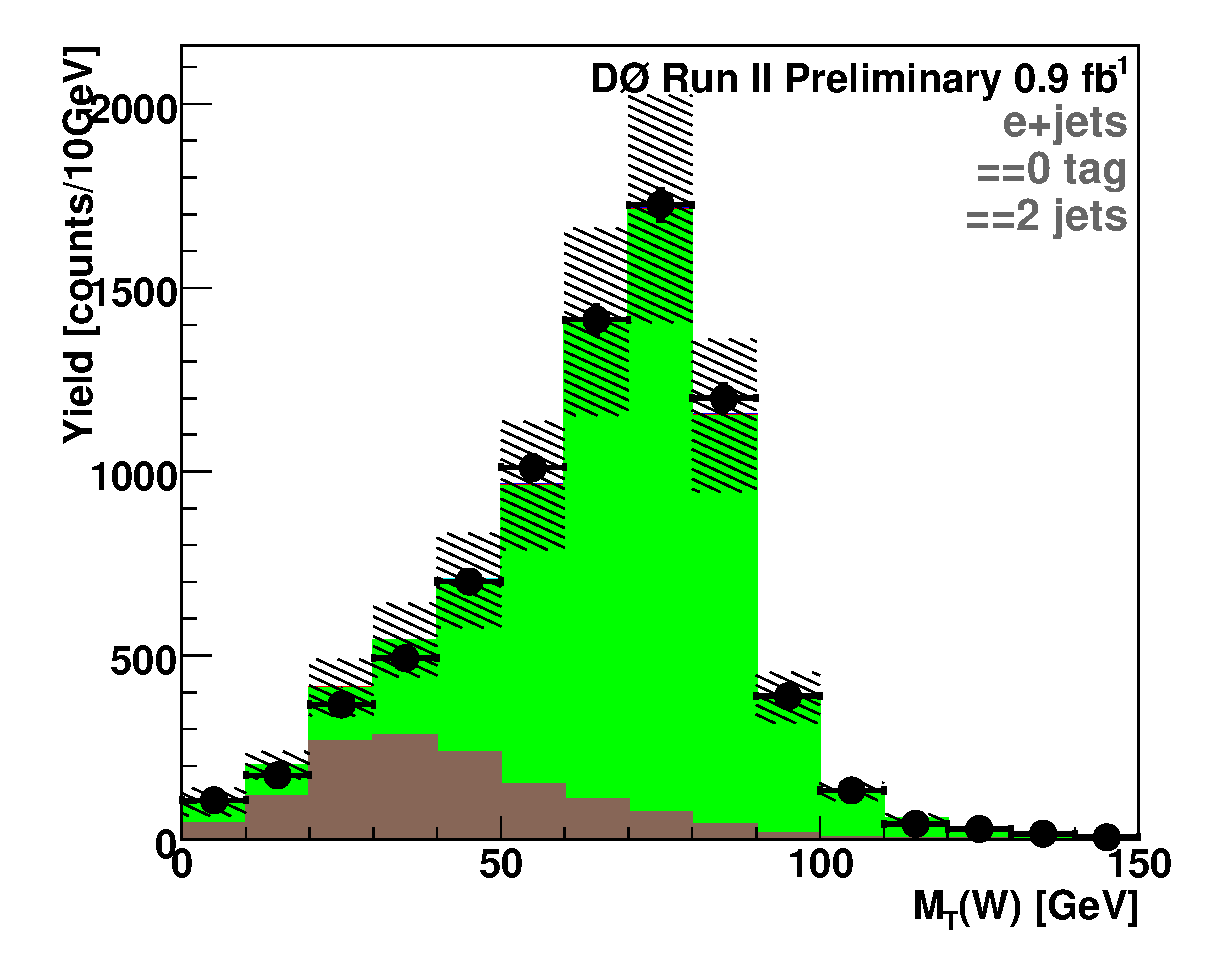
\includegraphics[width=0.32\textwidth]{figures/electron/CC_EqZeroTag_EqTwoJet_WTransverseMass.eps}  
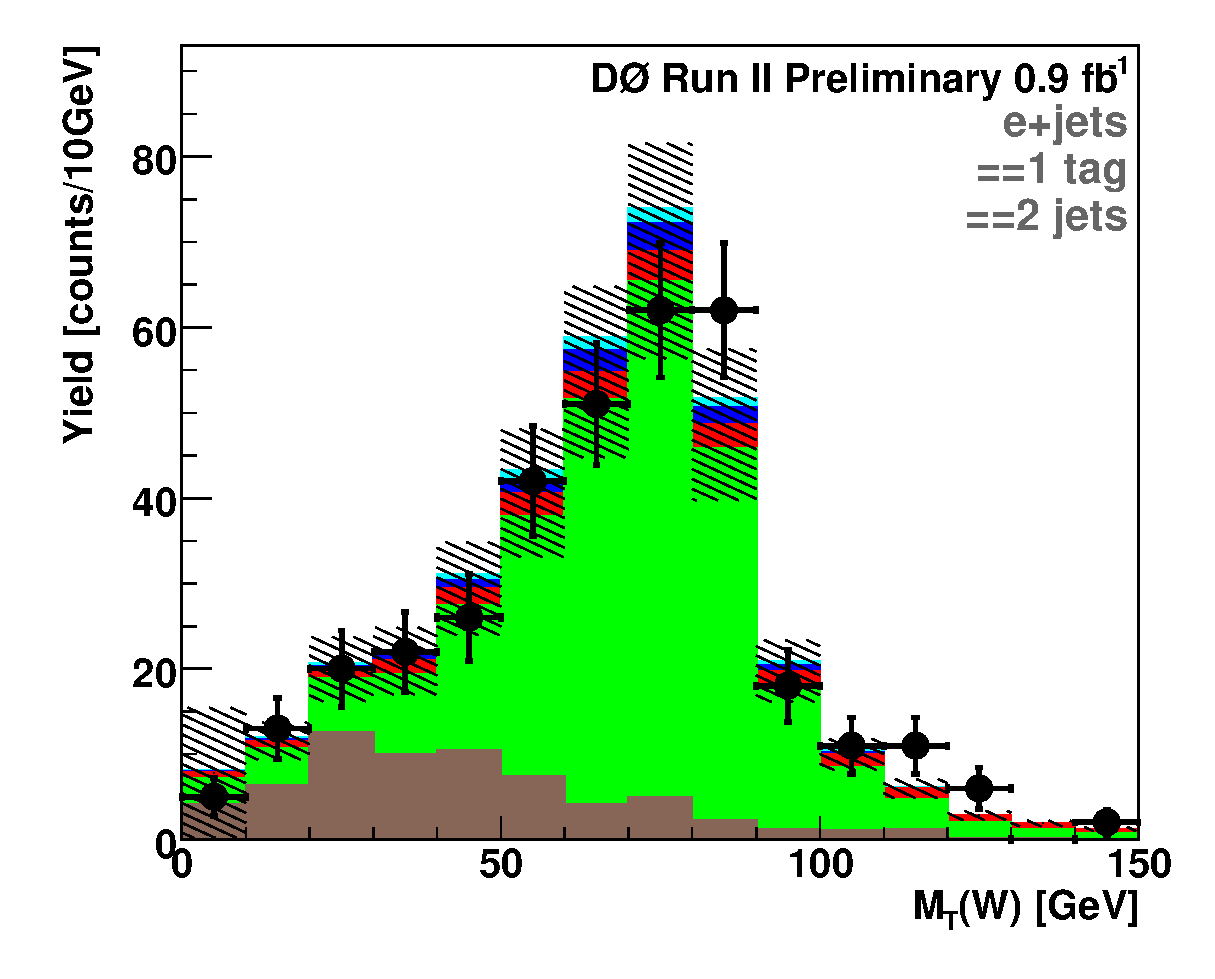
\includegraphics[width=0.32\textwidth]{figures/electron/CC_EqOneTag_EqTwoJet_WTransverseMass.eps}   
\includegraphics[width=0.32\textwidth]{figures/electron/CC_EqTwoTag_EqTwoJet_WTransverseMass.eps}   
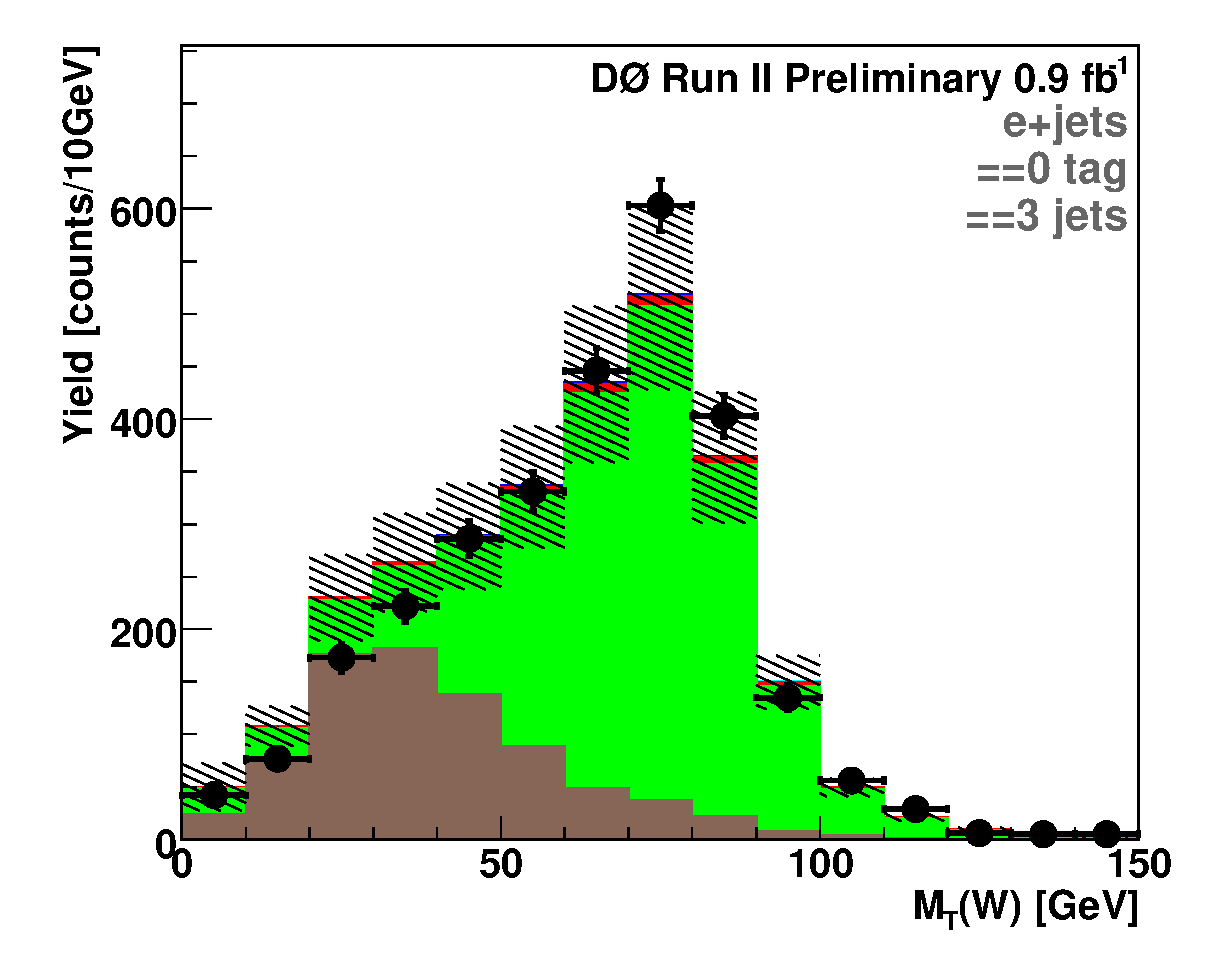
\includegraphics[width=0.32\textwidth]{figures/electron/CC_EqZeroTag_EqThreeJet_WTransverseMass.eps}
\includegraphics[width=0.32\textwidth]{figures/electron/CC_EqOneTag_EqThreeJet_WTransverseMass.eps} 
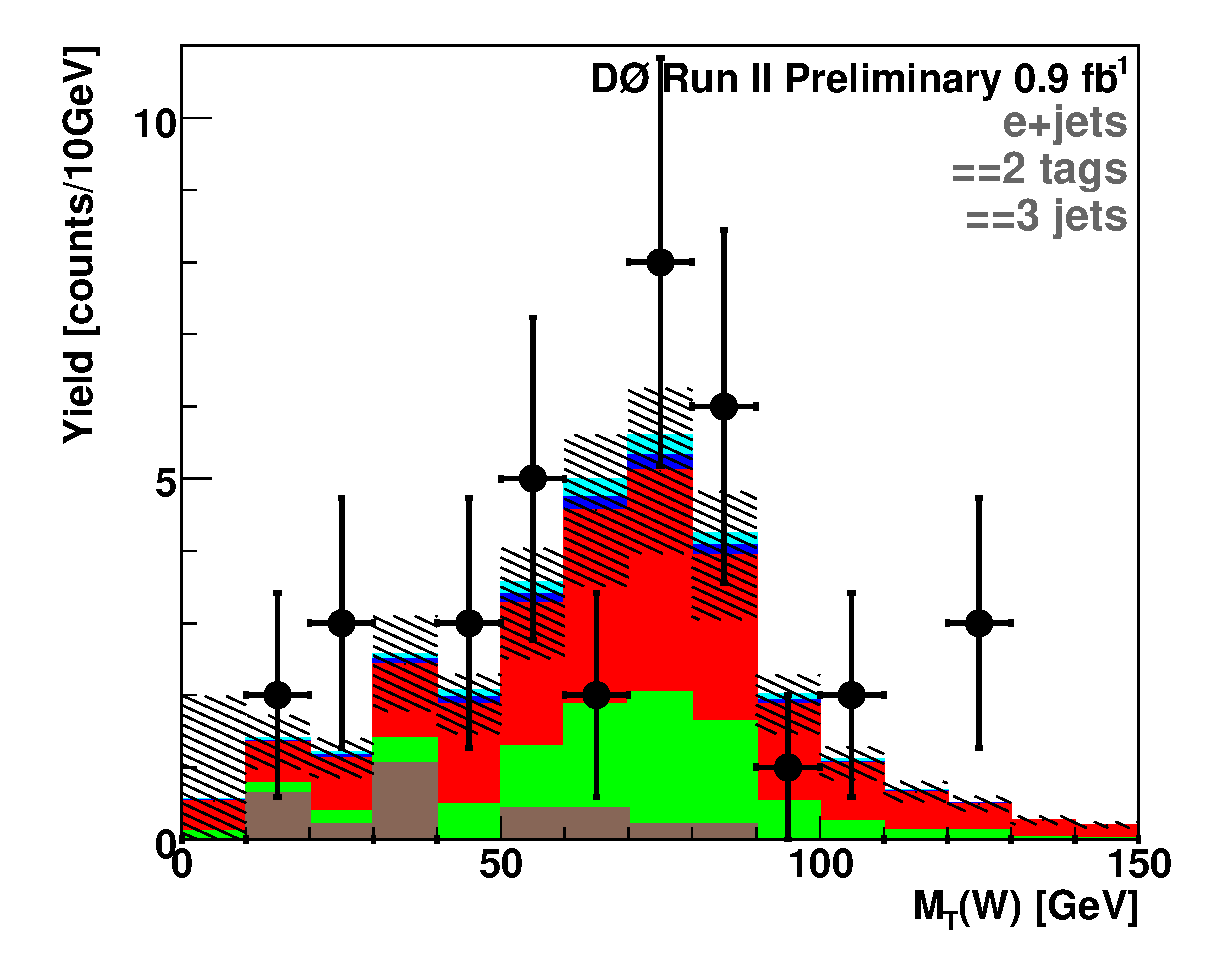
\includegraphics[width=0.32\textwidth]{figures/electron/CC_EqTwoTag_EqThreeJet_WTransverseMass.eps} 
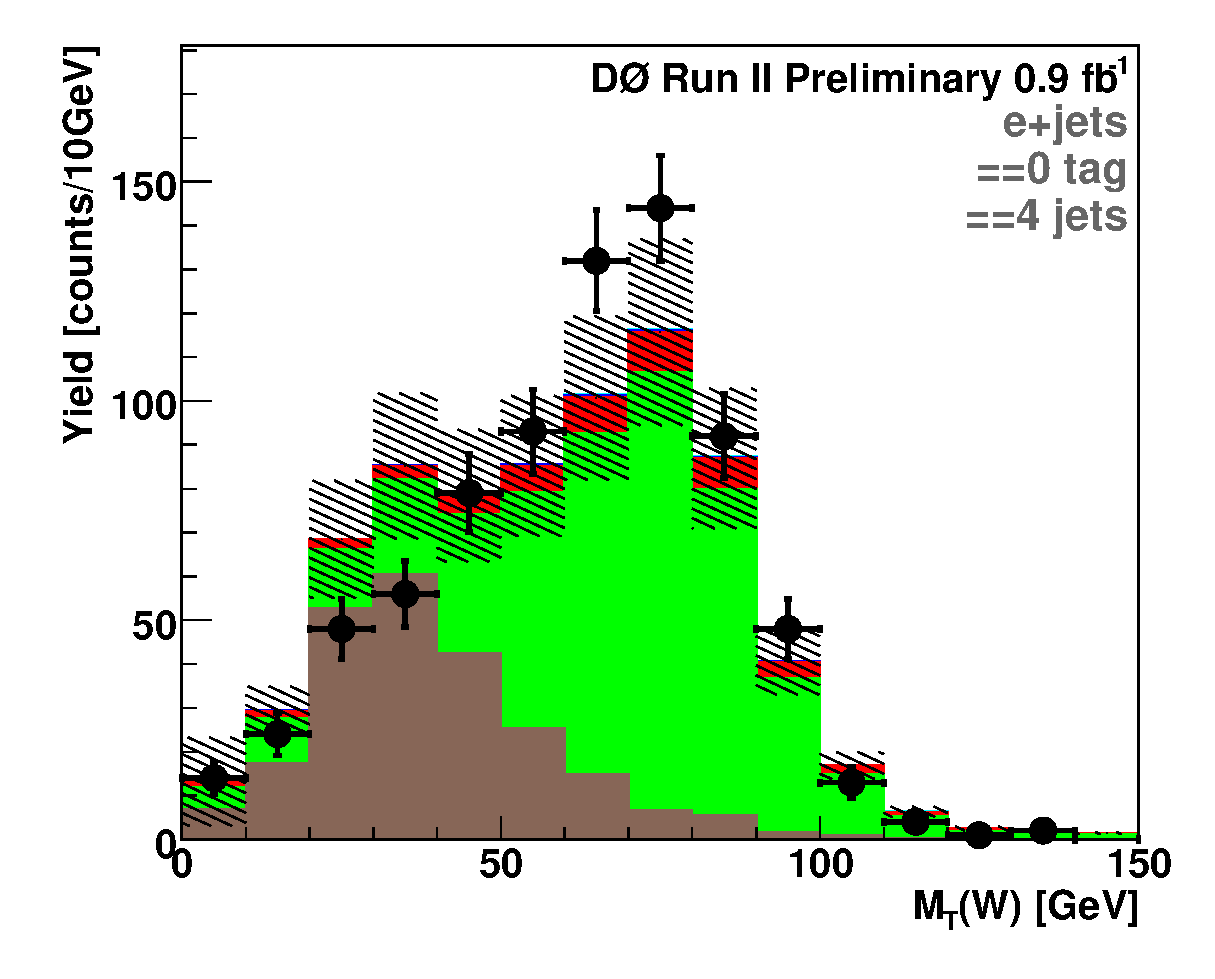
\includegraphics[width=0.32\textwidth]{figures/electron/CC_EqZeroTag_EqFourJet_WTransverseMass.eps} 
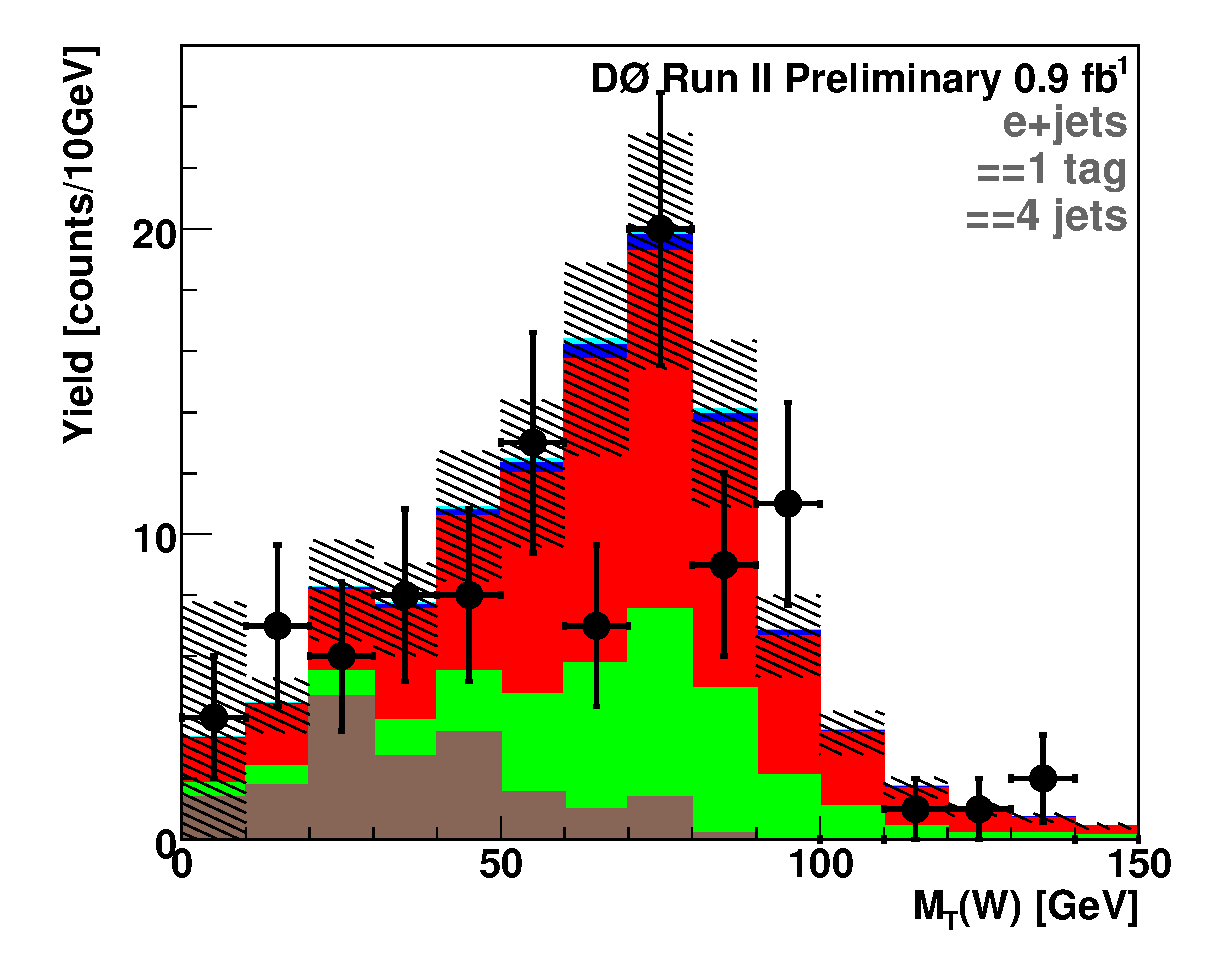
\includegraphics[width=0.32\textwidth]{figures/electron/CC_EqOneTag_EqFourJet_WTransverseMass.eps}  
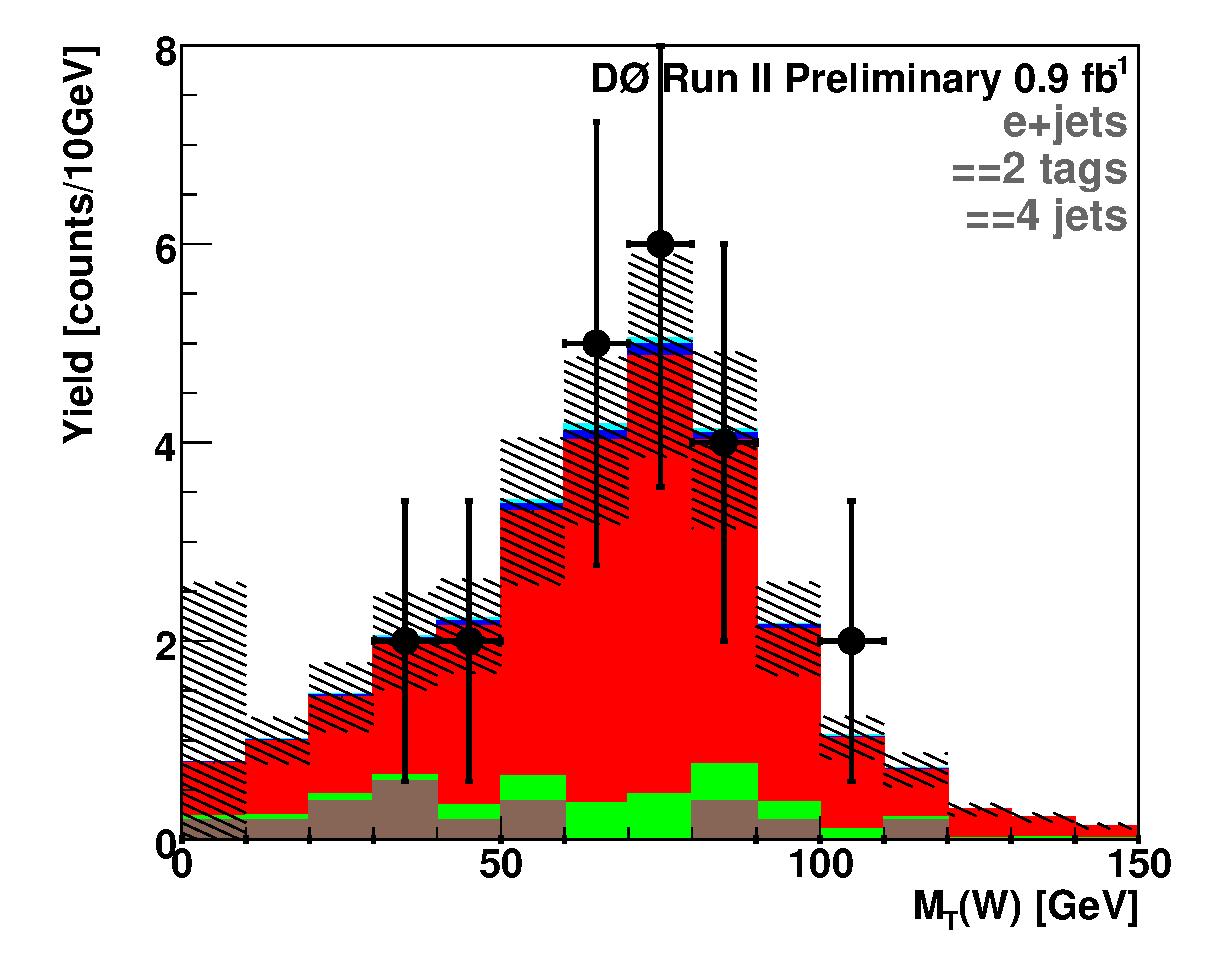
\includegraphics[width=0.32\textwidth]{figures/electron/CC_EqTwoTag_EqFourJet_WTransverseMass.eps}  
\vspace{-0.1in}
\caption[MTWelectron]{The $W$~boson transverse mass distributions for
the electron channel event samples after selection with zero tagged
jets (left column), one tagged jet (middle column), and two tagged
jets (right column). Events in the first row have one jet, in the
second row they have two jets, in the third row, three jets, and in
the fourth row, four jets.}
\label{MTW-electron}
\end{figure}

\clearpage

\begin{center}
W TRANSVERSE MASS IN THE MUON CHANNEL
\end{center}

\begin{figure}[!h!tbp]
\includegraphics[width=0.32\textwidth]{figures/muon/mu_EqZeroTag_EqOneJet_WTransverseMass.eps}  
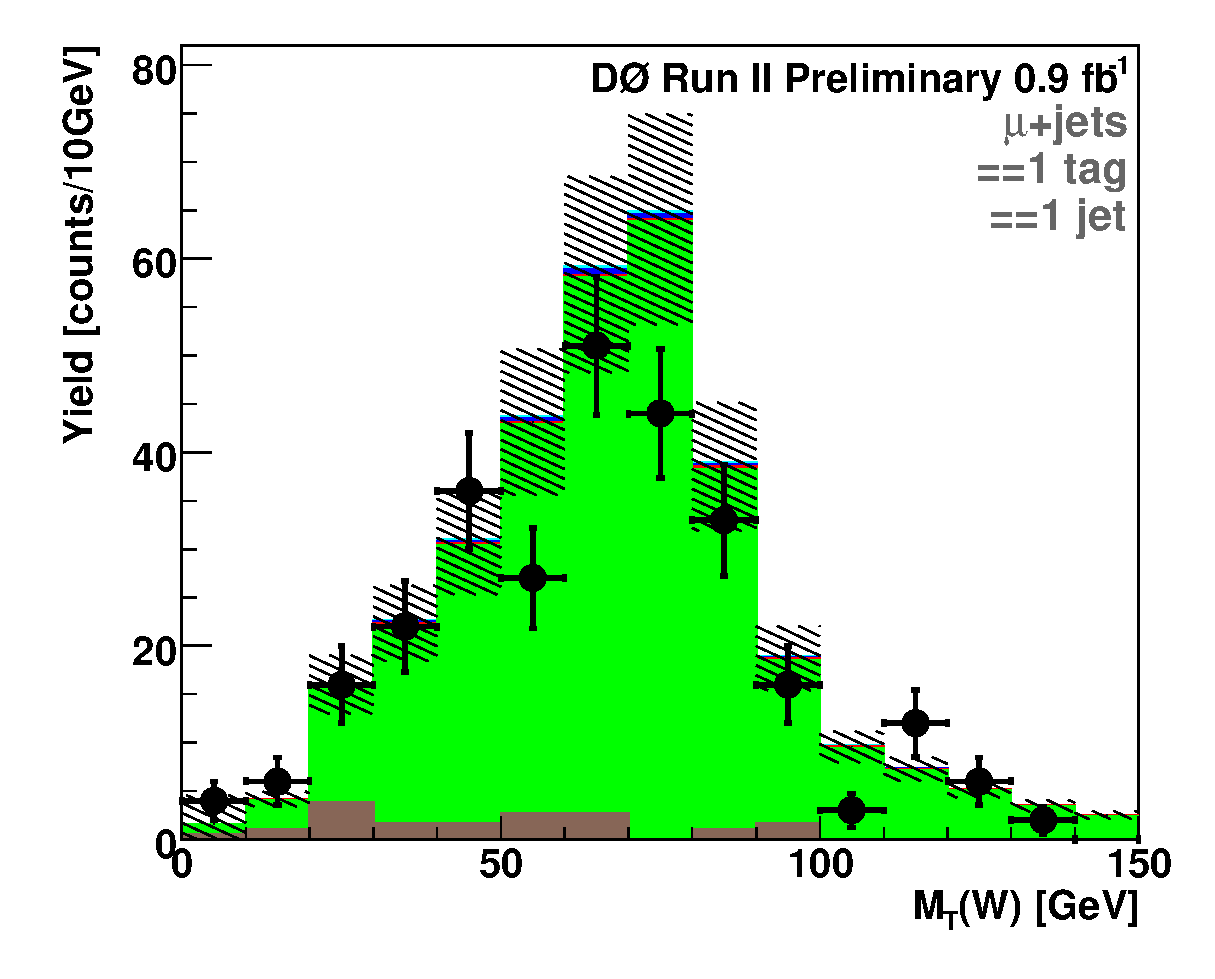
\includegraphics[width=0.32\textwidth]{figures/muon/mu_EqOneTag_EqOneJet_WTransverseMass.eps}   

\includegraphics[width=0.32\textwidth]{figures/muon/WTransverseMass_placeholder.eps}            
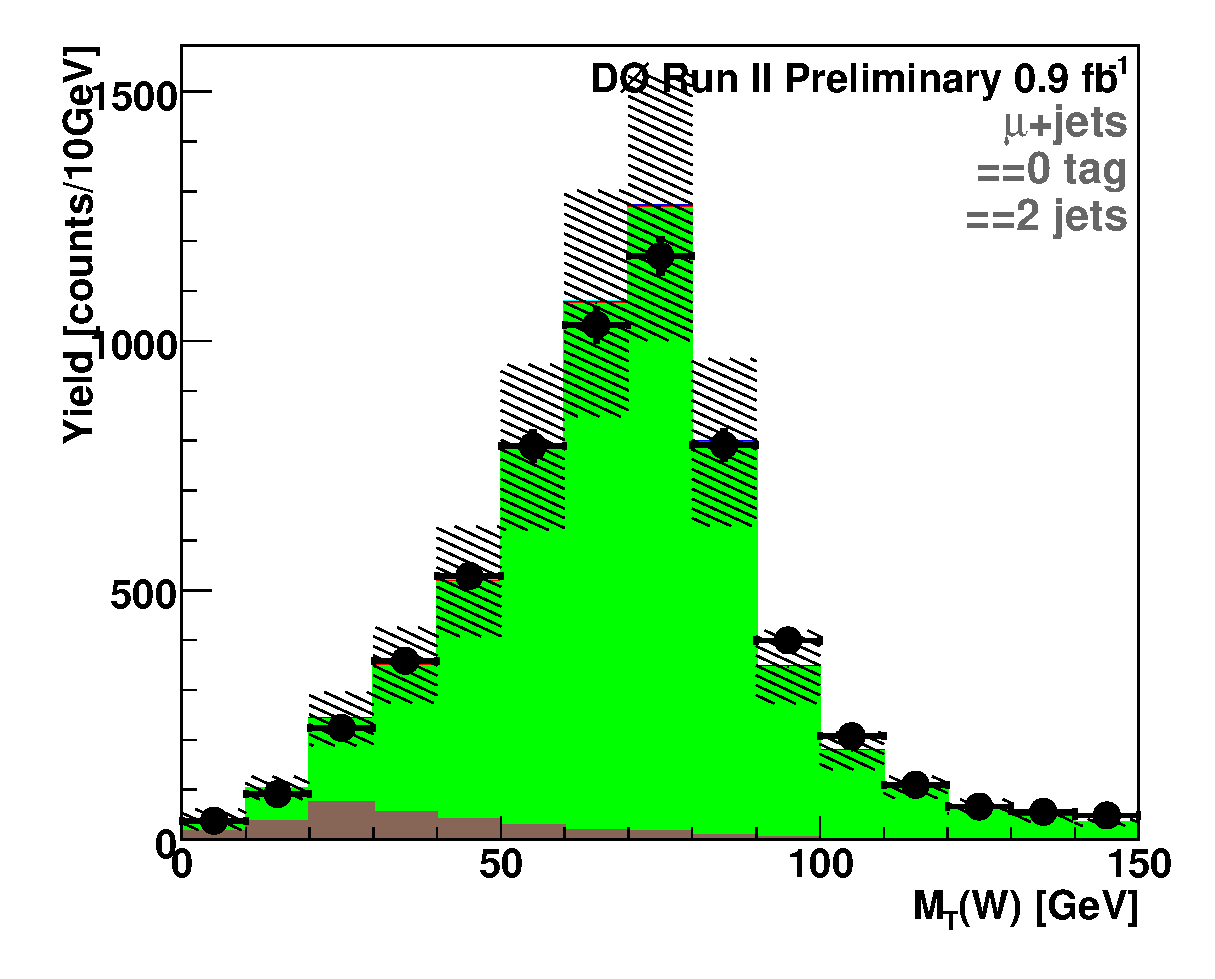
\includegraphics[width=0.32\textwidth]{figures/muon/mu_EqZeroTag_EqTwoJet_WTransverseMass.eps}  
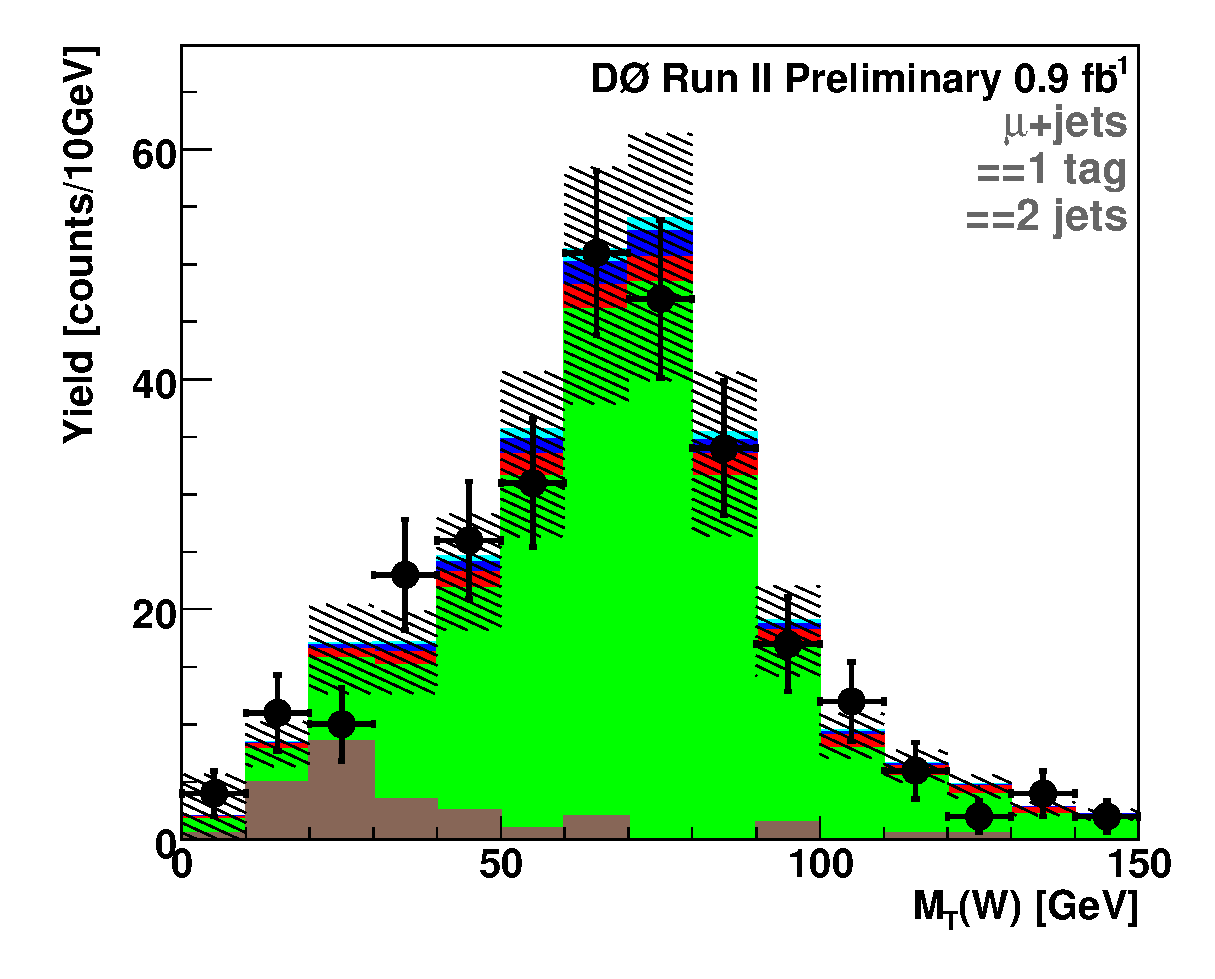
\includegraphics[width=0.32\textwidth]{figures/muon/mu_EqOneTag_EqTwoJet_WTransverseMass.eps}   
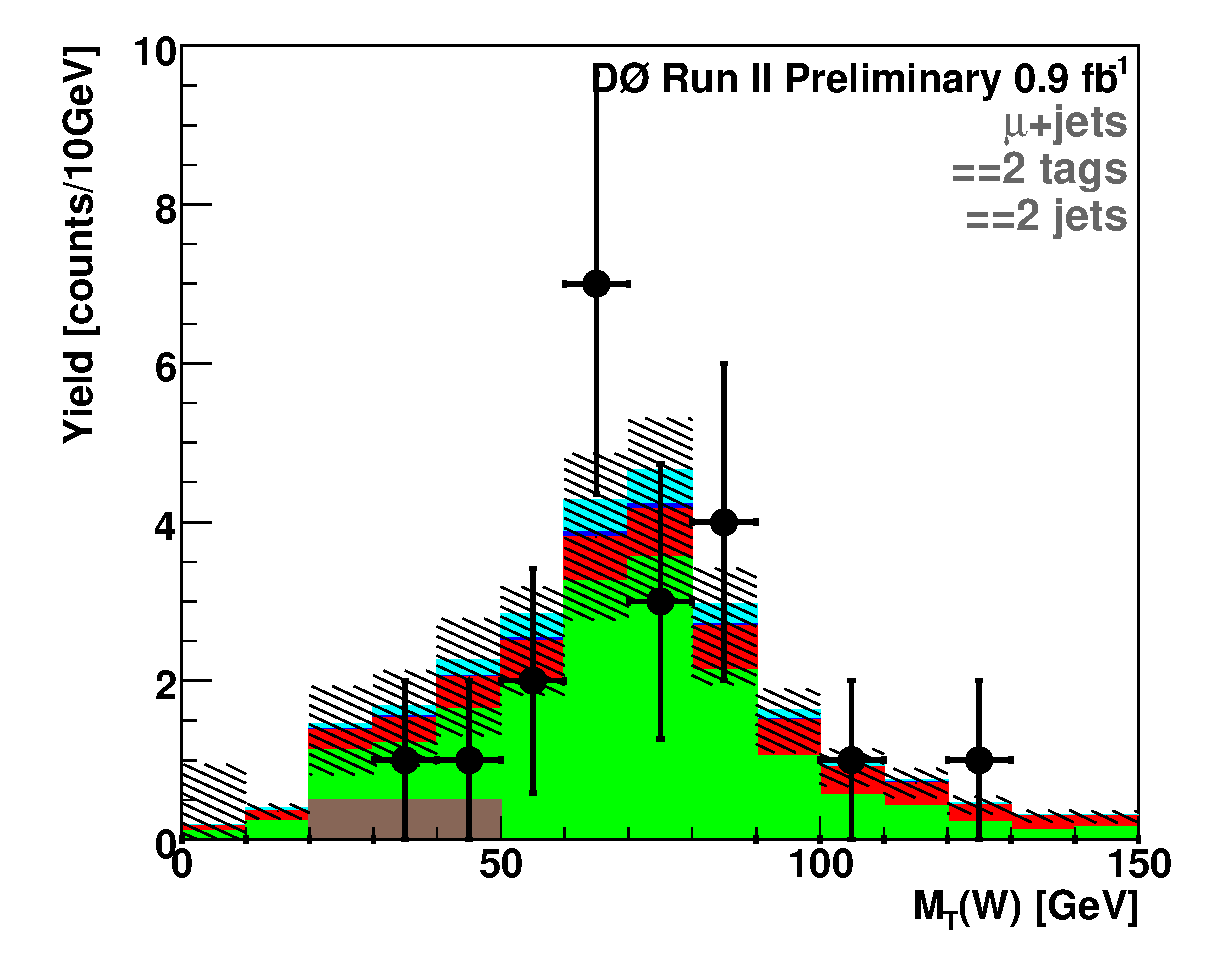
\includegraphics[width=0.32\textwidth]{figures/muon/mu_EqTwoTag_EqTwoJet_WTransverseMass.eps}   
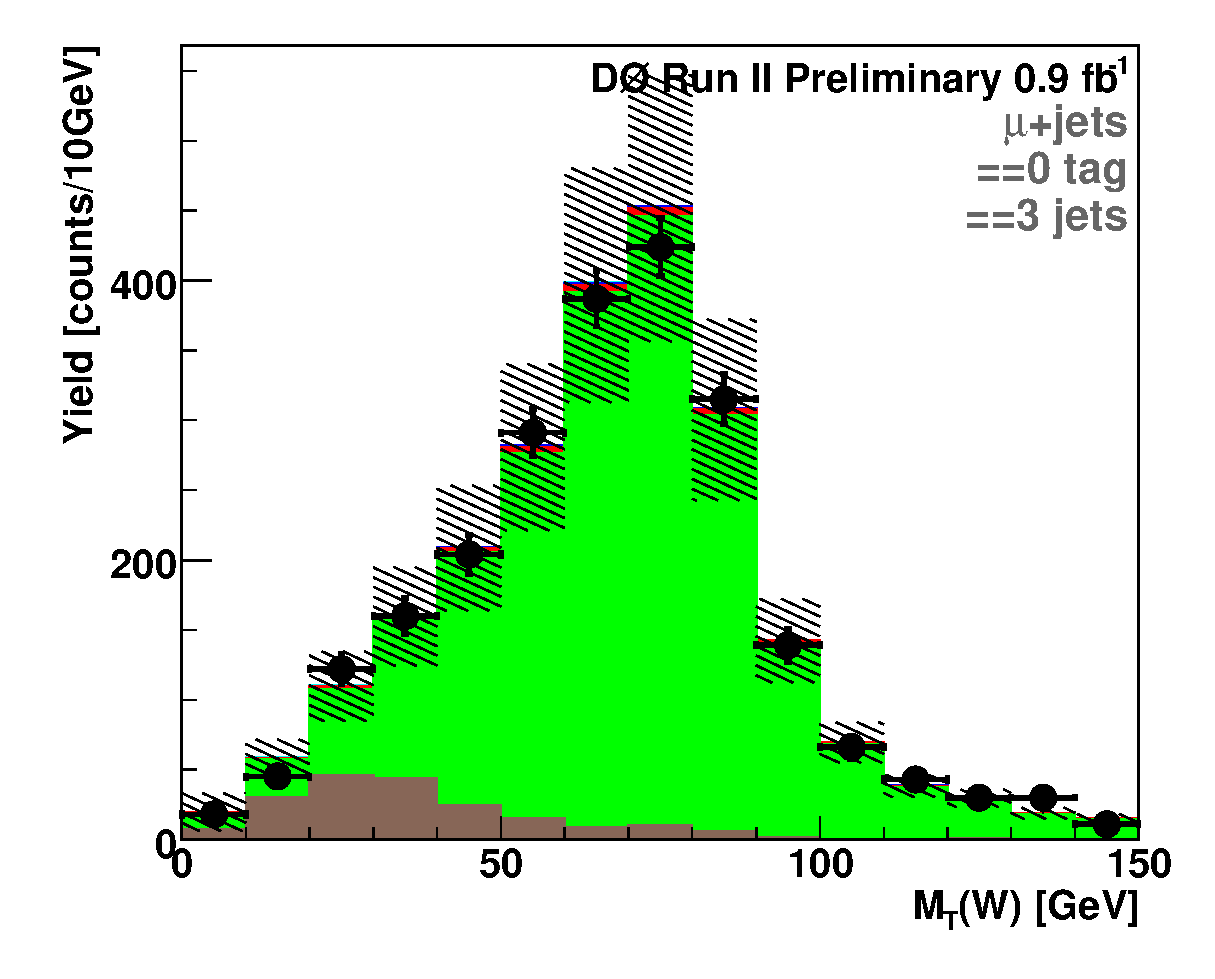
\includegraphics[width=0.32\textwidth]{figures/muon/mu_EqZeroTag_EqThreeJet_WTransverseMass.eps}
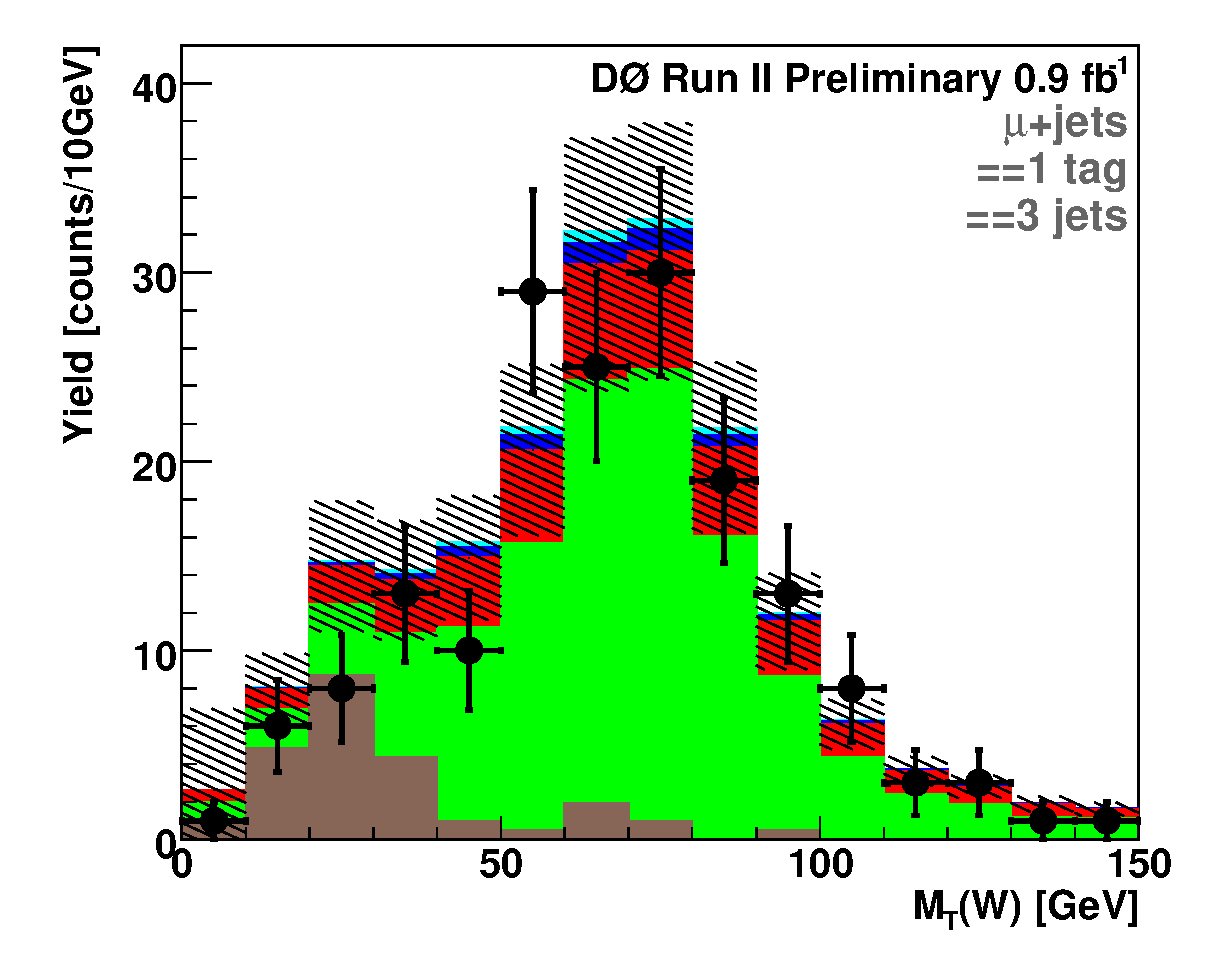
\includegraphics[width=0.32\textwidth]{figures/muon/mu_EqOneTag_EqThreeJet_WTransverseMass.eps} 
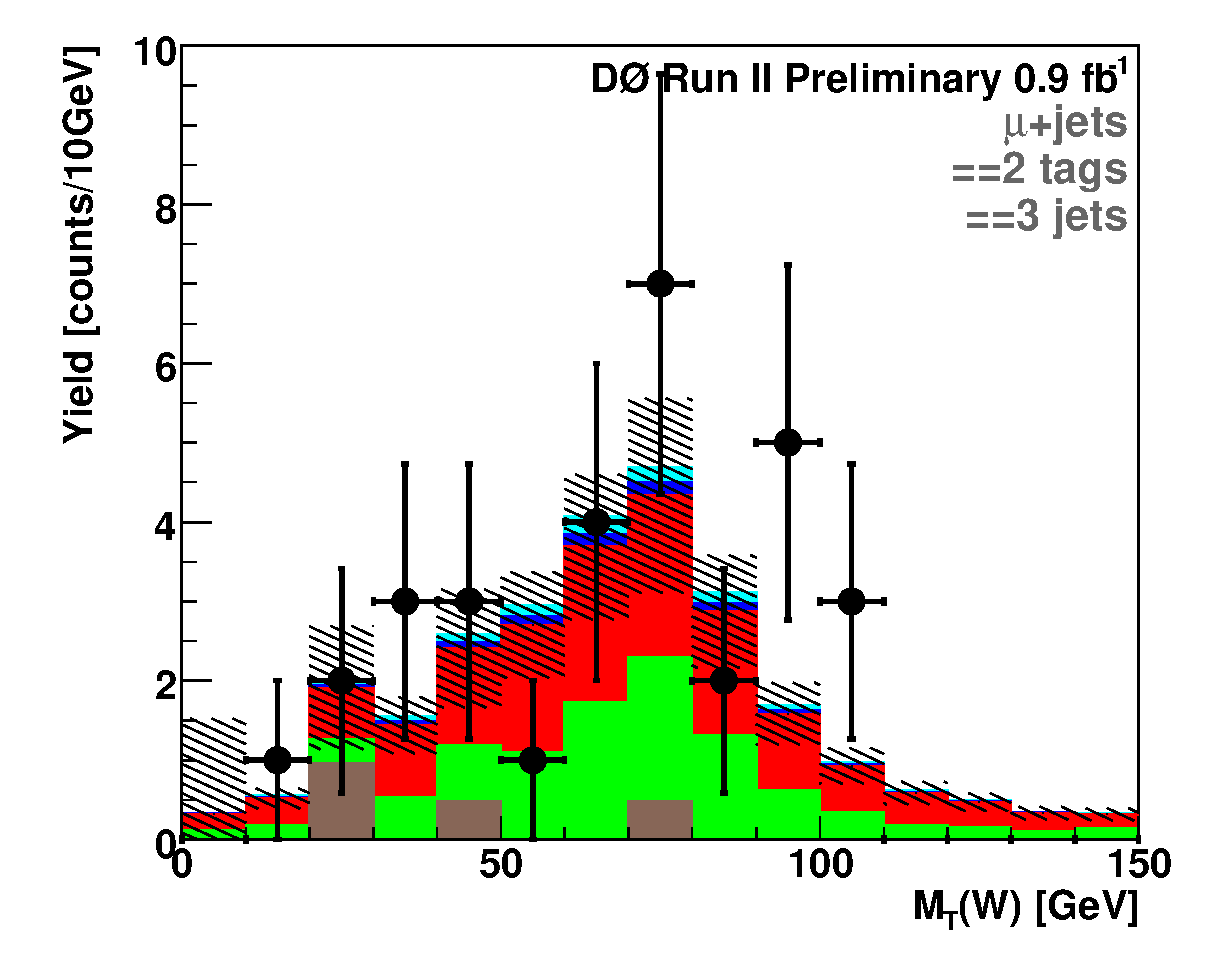
\includegraphics[width=0.32\textwidth]{figures/muon/mu_EqTwoTag_EqThreeJet_WTransverseMass.eps} 
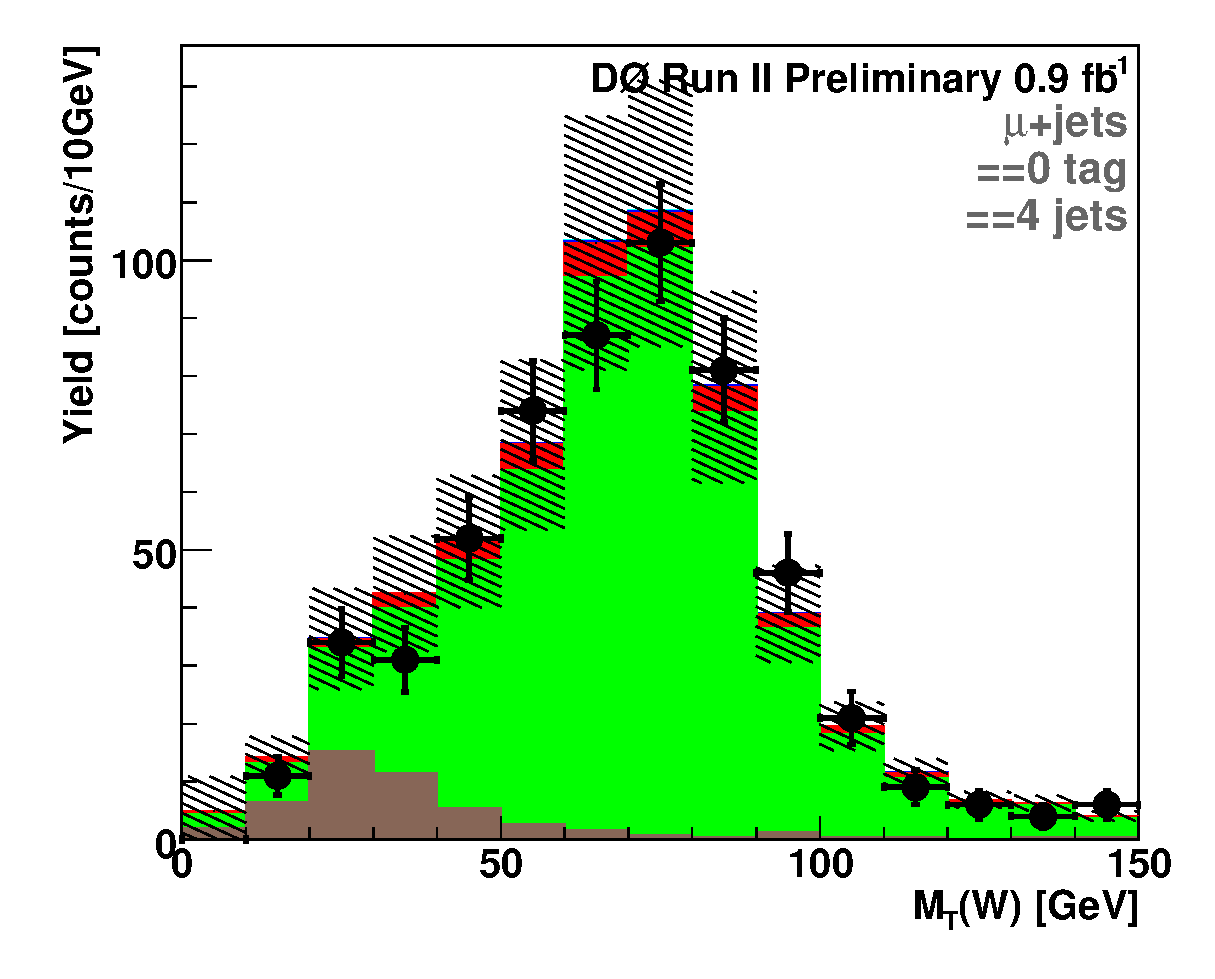
\includegraphics[width=0.32\textwidth]{figures/muon/mu_EqZeroTag_EqFourJet_WTransverseMass.eps} 
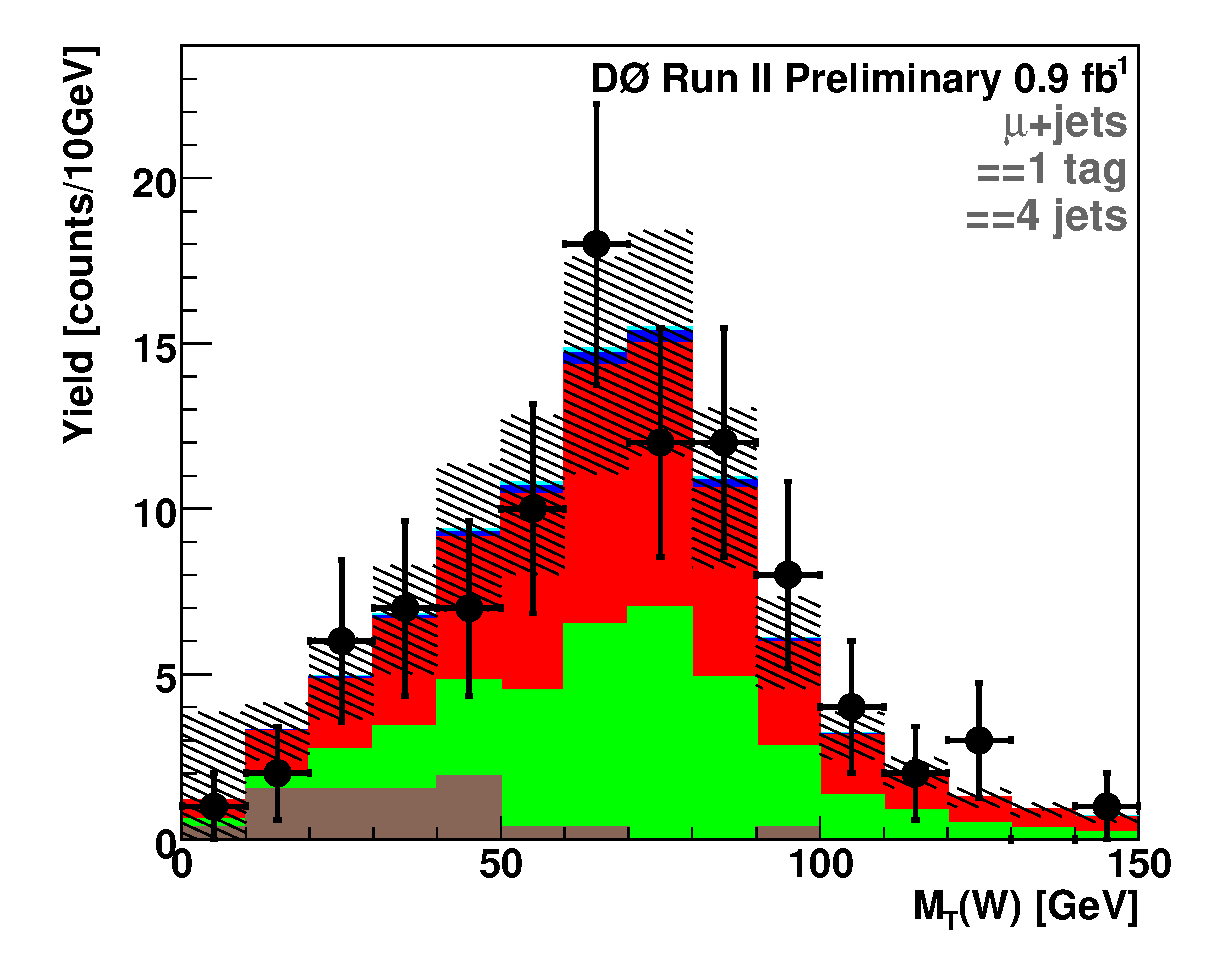
\includegraphics[width=0.32\textwidth]{figures/muon/mu_EqOneTag_EqFourJet_WTransverseMass.eps}  
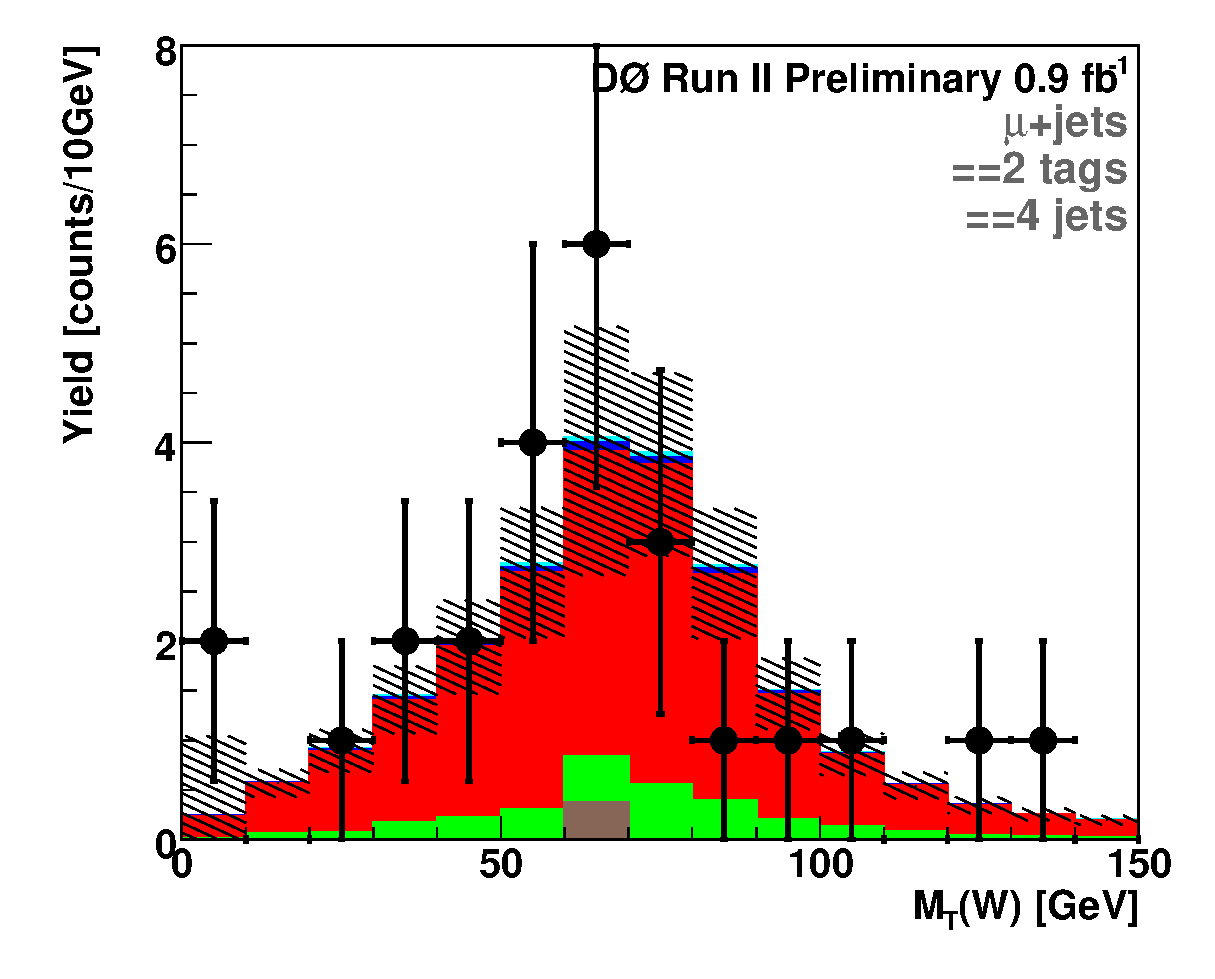
\includegraphics[width=0.32\textwidth]{figures/muon/mu_EqTwoTag_EqFourJet_WTransverseMass.eps}  
\vspace{-0.1in}
\caption[MTWmuon]{The $W$~boson transverse mass distributions for
the muon channel event samples after selection with zero tagged
jets (left column), one tagged jet (middle column), and two tagged
jets (right column). Events in the first row have one jet, in the
second row they have two jets, in the third row, three jets, and in
the forth row, four jets.}
\label{MTW-muon}
\end{figure}


%---------------------------------------------------------------------
%---------------------------------------------------------------------
% Summary of systematic uncertainties
\clearpage
%---------------------------------------------------------------------
%  Writeup of the improved search of Run II data for single top quark
%  production at DZero.
%  Started: Oct 2006
%  Authors: The Single Top Working Group
%---------------------------------------------------------------------
%

\section{Systematic Uncertainties}
\label{systematics}

Systematic uncertainties enter the single top calculations in two
ways: as uncertainty on the normalization of the background samples;
and as effects that change the shapes of the distributions of those
samples and the shapes of the expected signal distributions.

Table~\ref{tab:generalsys} summarises the relative uncertainties on
each of the sources described below. Detailed tables of uncertainties
for each individual channel are listed in Appendix~6.

We have considered the following systematic uncertainties in the
analysis:

\begin{itemize}
\item {\bf Integrated luminosity} \\ 
The error on the luminosity estimate affects the signal and $\ttbar$
yields.

\item {\bf Theoretical cross sections} \\ 
The uncertainty on the cross section for signal and $\ttbar$ includes
the theoretical error and the uncertainty from the top quark mass
uncertainty.

\item {\bf Trigger efficiency} \\
The trigger efficiency as a function of $\pt$ for each object in an MC
event is shifted up and down by one standard deviation and the weight
of the event recalculated. This shift is taken as an overall constant
systematic error on the MC acceptance.

\item {\bf Primary vertex selection efficiency} \\
The primary vertex selection efficiency in data and MC are not the
same. We assign a systematic uncertainty for the difference on the $z$
position of the primary vertex taking into account the beam profile
along the longitudinal direction~\cite{beamshifts}.

\item {\bf Jet reconstruction and identification} \\
The dependence of the efficiency on the number and the $\eta$ of the
jets is taken into account.

\item {\bf Jet energy scale and jet energy resolution} \\
The JES correction is raised and lowered by one standard deviation and
the whole analysis repeated. In the data, the JES uncertaintiy
contains the jet energy resolution uncertainty. But in the Monte Carlo
the jet energy resolution uncertainty is not taken into account in the
JES uncertainty. To account for this, the Monte Carlo energy smearing
is varied by the size of the jet energy resolution in MC. This
uncertainty affects the acceptance and the shapes of the
distributions.

\item {\bf Jet fragmentation} \\
This systematic error covers the difference in the jet fragmentation
models of {\sc pythia} and {\sc herwig} as well as the uncertainty in
the modeling of initial-state and final-state radiation.

\item {\bf Electron reconstruction and identification efficiency} \\
The electron reconstruction and identification scale factor is
parametrized as a function of the distance between the electron and
the closest jet. The dependences on $\phi$ and $\pt$ of the electron
are included in the systematic error and also the limited statistics
in each bin of the parametrization.

\item {\bf Electron track matching and likelihood efficiency} \\
These scale factors are parametrized as a function of $\eta$ and
$\phi$, and the limited statistics of each bin, as well as the
dependence on the number of jets are taken as the total systematic
uncertainty.

\item {\bf Muon reconstruction and identification efficiency} \\
The MC scale factor uncertainties are estimated by the muon ID group
as coming from the tag/probe method, background subtraction, and
limited statistics in the parametrization.

\item {\bf Muon track matching and isolation} \\
The muon tracking uncertainty, estimated by the muon ID group,
includes uncertainties from the tag/probe method, background
substraction, luminosity and timing bias, and averaging over $\phi$
and the limited statistics in each bin of the scale factor. The muon
isolation uncertainty was estimated based on the scale factor
dependence with the number of jets; and covers the dependences not
taken into account like $\pt$ and $\eta$.

\item {\bf Matrix method normalization} \\
The determination of the number of real-lepton events in data is
affected by the uncertainties associated with the determination of the
probabilities for a loose lepton to be (mis)identified as a (fake)
real lepton, $\varepsilon_{\rm fake{\mbox{\small -}}{\rm lepton}}$ and
$\varepsilon_{\rm real{\mbox{\small -}}{\rm lepton}}$. It is also
affected by the limited statistics of the data sample. See
Ref.~\cite{matrix-method} for more details.

\item {\bf Heavy flavor ratio} \\
The error on the scale factor we apply to set the $Wbb$ and $Wcc$
contributions in the $W$+jets sample, as described in Appendix~3, is
estimated to cover several effects: dependence on the $b$-quark $\pt$,
the difference between the zero tag samples where it is estimated and the
signal samples where it is used, and the intrinsic uncertainty on the value of
the LO cross section it's being applied on. 

\item {\bf Monte Carlo tag-rate functions}\\
The uncertainty associated with the tag-rate functions is evaluated by
raising and lowering the tag rate by one standard deviation for both
the taggability and the tag rate components and determining the new
event tagging weight. The TRF uncertainties originate from several
sources: statistical errors of MC event sets; the assummed fraction of
heavy flavor in the MC QCD for the mistag rate determination; and the
parametrizations.
\end{itemize}

\vspace{-0.1in}
\begin{table}[h]
\begin{center}
\begin{minipage}{5 in}
\begin{ruledtabular}
\begin{tabular}{l|c||l|c}
\multicolumn{4}{c}{\underline{Relative Systematic Uncertainties}}\\
\hline
{\ttbar} cross section~~~~~~~~~~~~ & $18\%$  & Primary vertex                    &  $3\%$  \\
Luminosity                         &  $6\%$  & Electron reco * ID                &  $2\%$  \\
Electron trigger                   & $3\%$   & Electron trackmatch \& likelihood &  $5\%$  \\
Muon trigger                       & $6\%$   & Muon reco * ID                    &  $7\%$  \\
Jet energy scale                   &wide range&Muon trackmatch \& isolation      &  $2\%$  \\
Jet efficiency                     &  $2\%$  & $\varepsilon_{{\rm real-}e}$      &  $2\%$  \\
Jet fragmentation                  & 5--7$\%$& $\varepsilon_{{\rm real-}\mu}$    &  $2\%$  \\
Heavy flavor ratio                 & $30\%$  & $\varepsilon_{{\rm fake-}e}$      &3--40$\%$\\ 
Tag-rate functions                 &2--16$\%$& $\varepsilon_{{\rm fake-}\mu}$    &2--15$\%$
\end{tabular}
\end{ruledtabular}
\caption[gensys]{A summary of the relative systematic uncertainties
for each of the applied corrections and efficiencies. The uncertainty
shown is the error on the correction or the efficiency, before it has
been applied to the MC or data samples.}
\label{tab:generalsys}
\end{minipage}
\end{center}
\end{table}


%  email from Lisa
% ======================================
% Muon channel
% ==============

% 1. Muon ID SF
% (a) Systematic uncertainty estimated by muonID group - 0.7%.
% It includes uncertainties from tag/probe method, background
% subtraction, binning
% (b) Systematic uncertainty coming from the limited statistics
% in each bin of 2D histogram - 7%.
% Second uncertainty is overestimated because we treat errors in
% each bin as fully correlated.
% But we prefer to be concervative for now (if it does not kills
% the analysis, of course) because we do not have a better way to
% estimate it.
% Total - 7%

% 2. Muon tracking SF
% (a) Systematic uncertainty estimated by muonID group - 0.7%.
% It includes uncertainties from tag/probe method, background
% subtraction, binning, lumi and time bias, averaging over phi.
% (b) Systematic uncertainty coming from the limited statistics
% in each bin of 1D histogram - 1.3%.
% Total - 1.5%

% 3. Muon isolation SF
% This systematic uncertainty was not estimated by muonID group.
% We estimated it from the plot showing dependence of isolation SF
% vs # of jets (this is the spc file we are using) and it is 2%.
% We also double checked that 2% covers the dependences we are not
% taking into accout (vs eta and pt) which are available in muon
% certification note.

% Total systematics from all sources on the muon: 7.4% (was 5.1%
% in p14).


% =========================================
% Electron channel
% ==============
% The estimate of the systematic uncertainties from EMID group is
% not yet available.

% 1. EM preselection SF (includes emid 10,11, isolation, emfraction)
% (a) Systematic uncertainty coming from the dependencies we do not
% take into account (phi, pt) - 2%
% (b) Systematic uncertainty coming from the limited statistics in
% each bin of 1D histogram - 1%.
% Total - 2.2%

% 2. EM postselection SF (includes hmatrix, trak-match and LH)
% (a) Systematic uncertainty coming from the dependence on the
% number of jets which was not taken into account - 4%
% (b) Systematic uncertainty coming from the limited statistics
% in each bin of 2D histogram - 3%.
% Total - 5%

% Total systematics from all sources on the electron: 5.5% (was 3.2%
% in p14).


% ========================================
% Primary vertex
% ==================
% From D0 note 5142 and p14 SFs we extracted the following
% uncertainties on PV SF and vertex z position simulation:
% electron channel - 2.4%
% muon channel - 3%

% ========================================
% Uncertainty on the jet reconstruction efficiency SF
% =====================================
% Amnon has made a back of the envelope propagation of the new
% uncertainties he has just released on the ttbar efficiency and
% obtained 1.8% uncertainty. This number depends on the # of jets
% and the distribution of the jets vs eta. Given that single top
% has 2 or 3 jets but they are more forward (ICD and EC regions
% have higher uncrrtainties) I obtained average uncertainty for
% single top of 1.5%.



%---------------------------------------------------------------------
%---------------------------------------------------------------------
% Statistical analysis, fitting, and results
% for the boosted decision trees analysis
\clearpage
\input{results_DT_F06}

%---------------------------------------------------------------------
%---------------------------------------------------------------------
% Statistical analysis, fitting, and results
% for the matrix elements analysis
\clearpage
\input{results_ME_F06}

%---------------------------------------------------------------------
%---------------------------------------------------------------------
% Statistical analysis, fitting, and results
% for the MLPfit neural networks analysis
%\clearpage
%\input{results_NN_F06}

%---------------------------------------------------------------------
%---------------------------------------------------------------------
% Statistical analysis, fitting, and results
% for the Bayesian networks analysis
\clearpage
\input{results_BN_F06}

%---------------------------------------------------------------------
%---------------------------------------------------------------------
% Conclusions (summary for those in a hurry)
\clearpage
\input{conclusionsF06}

%---------------------------------------------------------------------
%---------------------------------------------------------------------
%---------------------------------------------------------------------
%---------------------------------------------------------------------
%% Description of triggers                  # 1
\clearpage
%---------------------------------------------------------------------
%  Writeup of the improved search of Run II data for single top quark
%  production at DZero.
%  Started: Oct 2006
%  Authors: The Single Top Working Group
%---------------------------------------------------------------------
%

\appendix
\section*{Appendix 1 --- Trigger Definitions and Simulation}
\label{appendix-triggers}

\subsection{Trigger Definitions}
Trigger requirements for the electron and muon analysis channels are
shown in Tables~\ref{electronchan-triggers} and
\ref{muonchan-triggers}. More details about these triggers can be found in
Refs.~\cite{top_trigger_web,d0_note_4512,d0_note_4978}.

\begin{table}[!h!tbp]
\begin{center}
\begin{ruledtabular}
\begin{tabular}{lc||ccc} 
\multicolumn{5}{c}{\hspace{0.1in}\underline{Electron Channel Triggers}}\vspace{0.1in}\\
Trigger Version & Trigger Name & Level 1 Condition & Level 2 Condition
& Level 3 Condition \\
\hline
 v8.0 -- v9.0  & EM15\_2JT15        & CEM(1,10)CJT(2,5) & EM(0.85,10)JET(2,10) & SHT(1,15)JET(2,15)          \\
 v9.0 -- v10.0 & EM15\_2JT15        & CEM(1,10)CJT(2,5) & EM(0.85,10)JET(2,10) & SH(1,15)JET(2,15)           \\
v10.0 -- v11.0 & EM15\_2JT15        & CEM(1,10)CJT(2,5) & EM(0.85,10)JET(2,10) & SH(1,15)JET(2,15)           \\
v11.0 -- v12.0 & EM15\_2JT15        & CEM(1,10)CJT(2,5) & EM(0.85,10)JET(2,10) & SH(1,15)JET(2,15)           \\
v12.0 -- v13.0 & E1\_SHT15\_2J20    & CEM(1,11)         & None                 & SHT(1,15)JET(2,20)          \\
v13.0 -- v13.3 & E1\_SHT15\_2J\_J25 & CEM(1,11)         & L2CALEM(15,x)        & SHT(1,15)JET(1,25)JET(2,20) \\
v13.3 -- v14.0 & E1\_SHT15\_2J\_J30 & CEM(1,11)         & L2CALEM(15,x)        & SHT(1,15)JET(1,30)JET(2,20) \\
v14.0 -- v15.0 & E1\_SHT15\_2J\_J25 & CEM(1,12)         & L2CALEM(15,x)        & SHT(1,15)JET(1,25)JET(2,20)
\end{tabular}
\end{ruledtabular}
\vspace{-0.1in}
\caption[eltriggers]{Definitions of triggers used in the
electron channel of the single top analysis.}
\label{electronchan-triggers}
\end{center}
\end{table}

\vspace{-0.25in}

\begin{table}[!h!tbp]
\begin{center}
\begin{ruledtabular}
\begin{tabular}{lc||ccc} 
\multicolumn{5}{c}{\hspace{0.1in}\underline{Muon Channel Triggers}}\vspace{0.1in}\\
Trigger Version & Trigger Name & Level 1 Condition & Level 2 Condition & Level 3 Condition \\
\hline
 v8.0 -- v9.0  & MU\_JT20\_L2M0   & mu1ptxatxx\_CJT(1,5) & MUON(1,med)          & JET(1,20)                 \\
 v9.0 -- v10.0 & MU\_JT20\_L2M0   & mu1ptxatxx\_CJT(1,5) & MUON(1,med)          & JET(1,20)                 \\
v10.0 -- v11.0 & MU\_JT20\_L2M0   & mu1ptxatxx\_CJT(1,5) & MUON(1,med)          & JET(1,20)                 \\
v11.0 -- v12.0 & MU\_JT20\_L2M0   & mu1ptxatxx\_CJT(1,5) & MUON(1,med)          & JET(1,20)                 \\
v12.0 -- v13.0 & MU\_JT25\_L2M0   & mu1ptxatxx\_CJT(1,3) & MUON(1,med)JET(1,10) & JET(1,25)                 \\
v13.0 -- v13.2 & MUJ2\_JT25       & mu1ptxatxx\_CJT(1,5) & MUON(1,med)JET(1,8)  & JET(1,25)                 \\
v13.2 -- v13.3 & MUJ2\_JT25\_LM3  & mu1ptxatlx\_CJT(1,5) & MUON(1,med)JET(1,8)  & JET(1,25)MUON(1,3.,loose) \\
v13.3 -- v14.0 & MUJ2\_JT30\_LM3  & mu1ptxatlx\_CJT(1,5) & MUON(1,med)JET(1,8)  & JET(1,30)MUON(1,3.,loose) \\
v14.0 -- v14.2 & MUJ1\_JT25\_LM3  & mu1ptxatlx\_CJT(1,5) & MUON(1,med)JET(1,8)  & JET(1,25)MUON(1,3.,loose) \\
v14.2 -- v14.3 & MUJ1\_JT25\_ILM3 & mu1ptxatlx\_CJT(1,5) & MUON(1,med)JET(1,8)  & JET(1,25)MUON(1,3.,loose) \\
                                  &                      &                      & ISO\_MUON(1oose)          \\
v14.3 -- v15.0 & MUJ1\_JT35\_LM3  & mu1ptxatlx\_CJT(1,5) & MUON(1,med)JET(1,8)  & JET(1,35)MUON(1,3.,loose) \\
\end{tabular}
\end{ruledtabular}
\vspace{-0.1in}
\caption[muonchantriggers]{Definitions of triggers used in the
muon channel of the single top analysis.}
\label{muonchan-triggers}
\end{center}
\end{table}

\vspace{-0.2in}
For the electron channel at Level 1, trigger term CEM(1,X) requires
that events must contain at least one electromagnetic trigger tower
with transverse energy $E_T > X$~GeV where $X = 10, 11,$ or 12, and
trigger term CJT(2,5) requires that events must contain at least two
calorimeter jet trigger towers with energy above 5~GeV. At Level 2,
EM(0.85,10) requires at least one Level 2 electromagnetic object with
$E_T > 10$~GeV and electromagnetic fraction greater than 0.85,
JET(2,10) requires at least two Level 2 jets with $E_T > 10$~GeV, and
L2CALEM(15,x) requires a standard Level 2 EM cluster with $E_T >
15$~GeV. At Level 3, SH(1,15) (SHT(1,15)) requires at least one
electron defined with a (tight) shower shape cut and $E_T > 15$~GeV,
JET(1,X) (JET(2,X)) requires at least one (two) Level 3 jet(s) with
$E_T > X$~GeV where $X = 15, 20, 25,$ or 30.

For the muon channel at Level 1, trigger term mu1ptxatxx (mu1ptxatlx)
requires that events must fire the single-muon trigger based on muon
scintillators with no (loose) wires, and CJT(1,X) requires at least
one calorimeter jet trigger tower with $E_T > X$~GeV where $X = 3$ or
5. At Level 2, MUON(1,med) requires one muon candidate with medium
quality, and JET(1,X) requires at least one Level 2 jet with $E_T >
X$~GeV where $X = 8$ or 10. At Level 3, JET(1,X) requires at least one
Level 3 jet with $E_T > X$~GeV where $X = 20, 25, 30,$ or 35,
MUON(1,3.,loose) requires one muon candidate with loose quality and
$p_T > 3$~GeV, and ISO\_MUON(1,3,loose) requires one isolated muon
candidate with loose quality and $p_T > 3$~GeV. The presence of
two Level 2 trigger terms in the v14.2 list indicates that events must
fire either of these terms.

\subsection{Trigger Simulation in Monte Carlo}
\label{trigger-simulation}

Objects in Monte Carlo events need to have the trigger inefficiencies
simulated. We do this by modifying the weight for each MC event using
trigger efficiency turn-on curves for each object measured on
data. This method does not determine if a Monte Carlo event passes or
fails the trigger, instead the probability of that event to fire the
trigger is calculated.  Details of the method and its implementation
can be found in Ref.~\cite{d0_note_4512,d0_note_4882,caf_trigger}. An
example electron turn-on curve versus $p_T$ is shown in
Fig.~\ref{trigger-turnons} together with an example muon turn-on curve
versus {\deta}.

\begin{figure}[!h!tbp]
\begin{center}
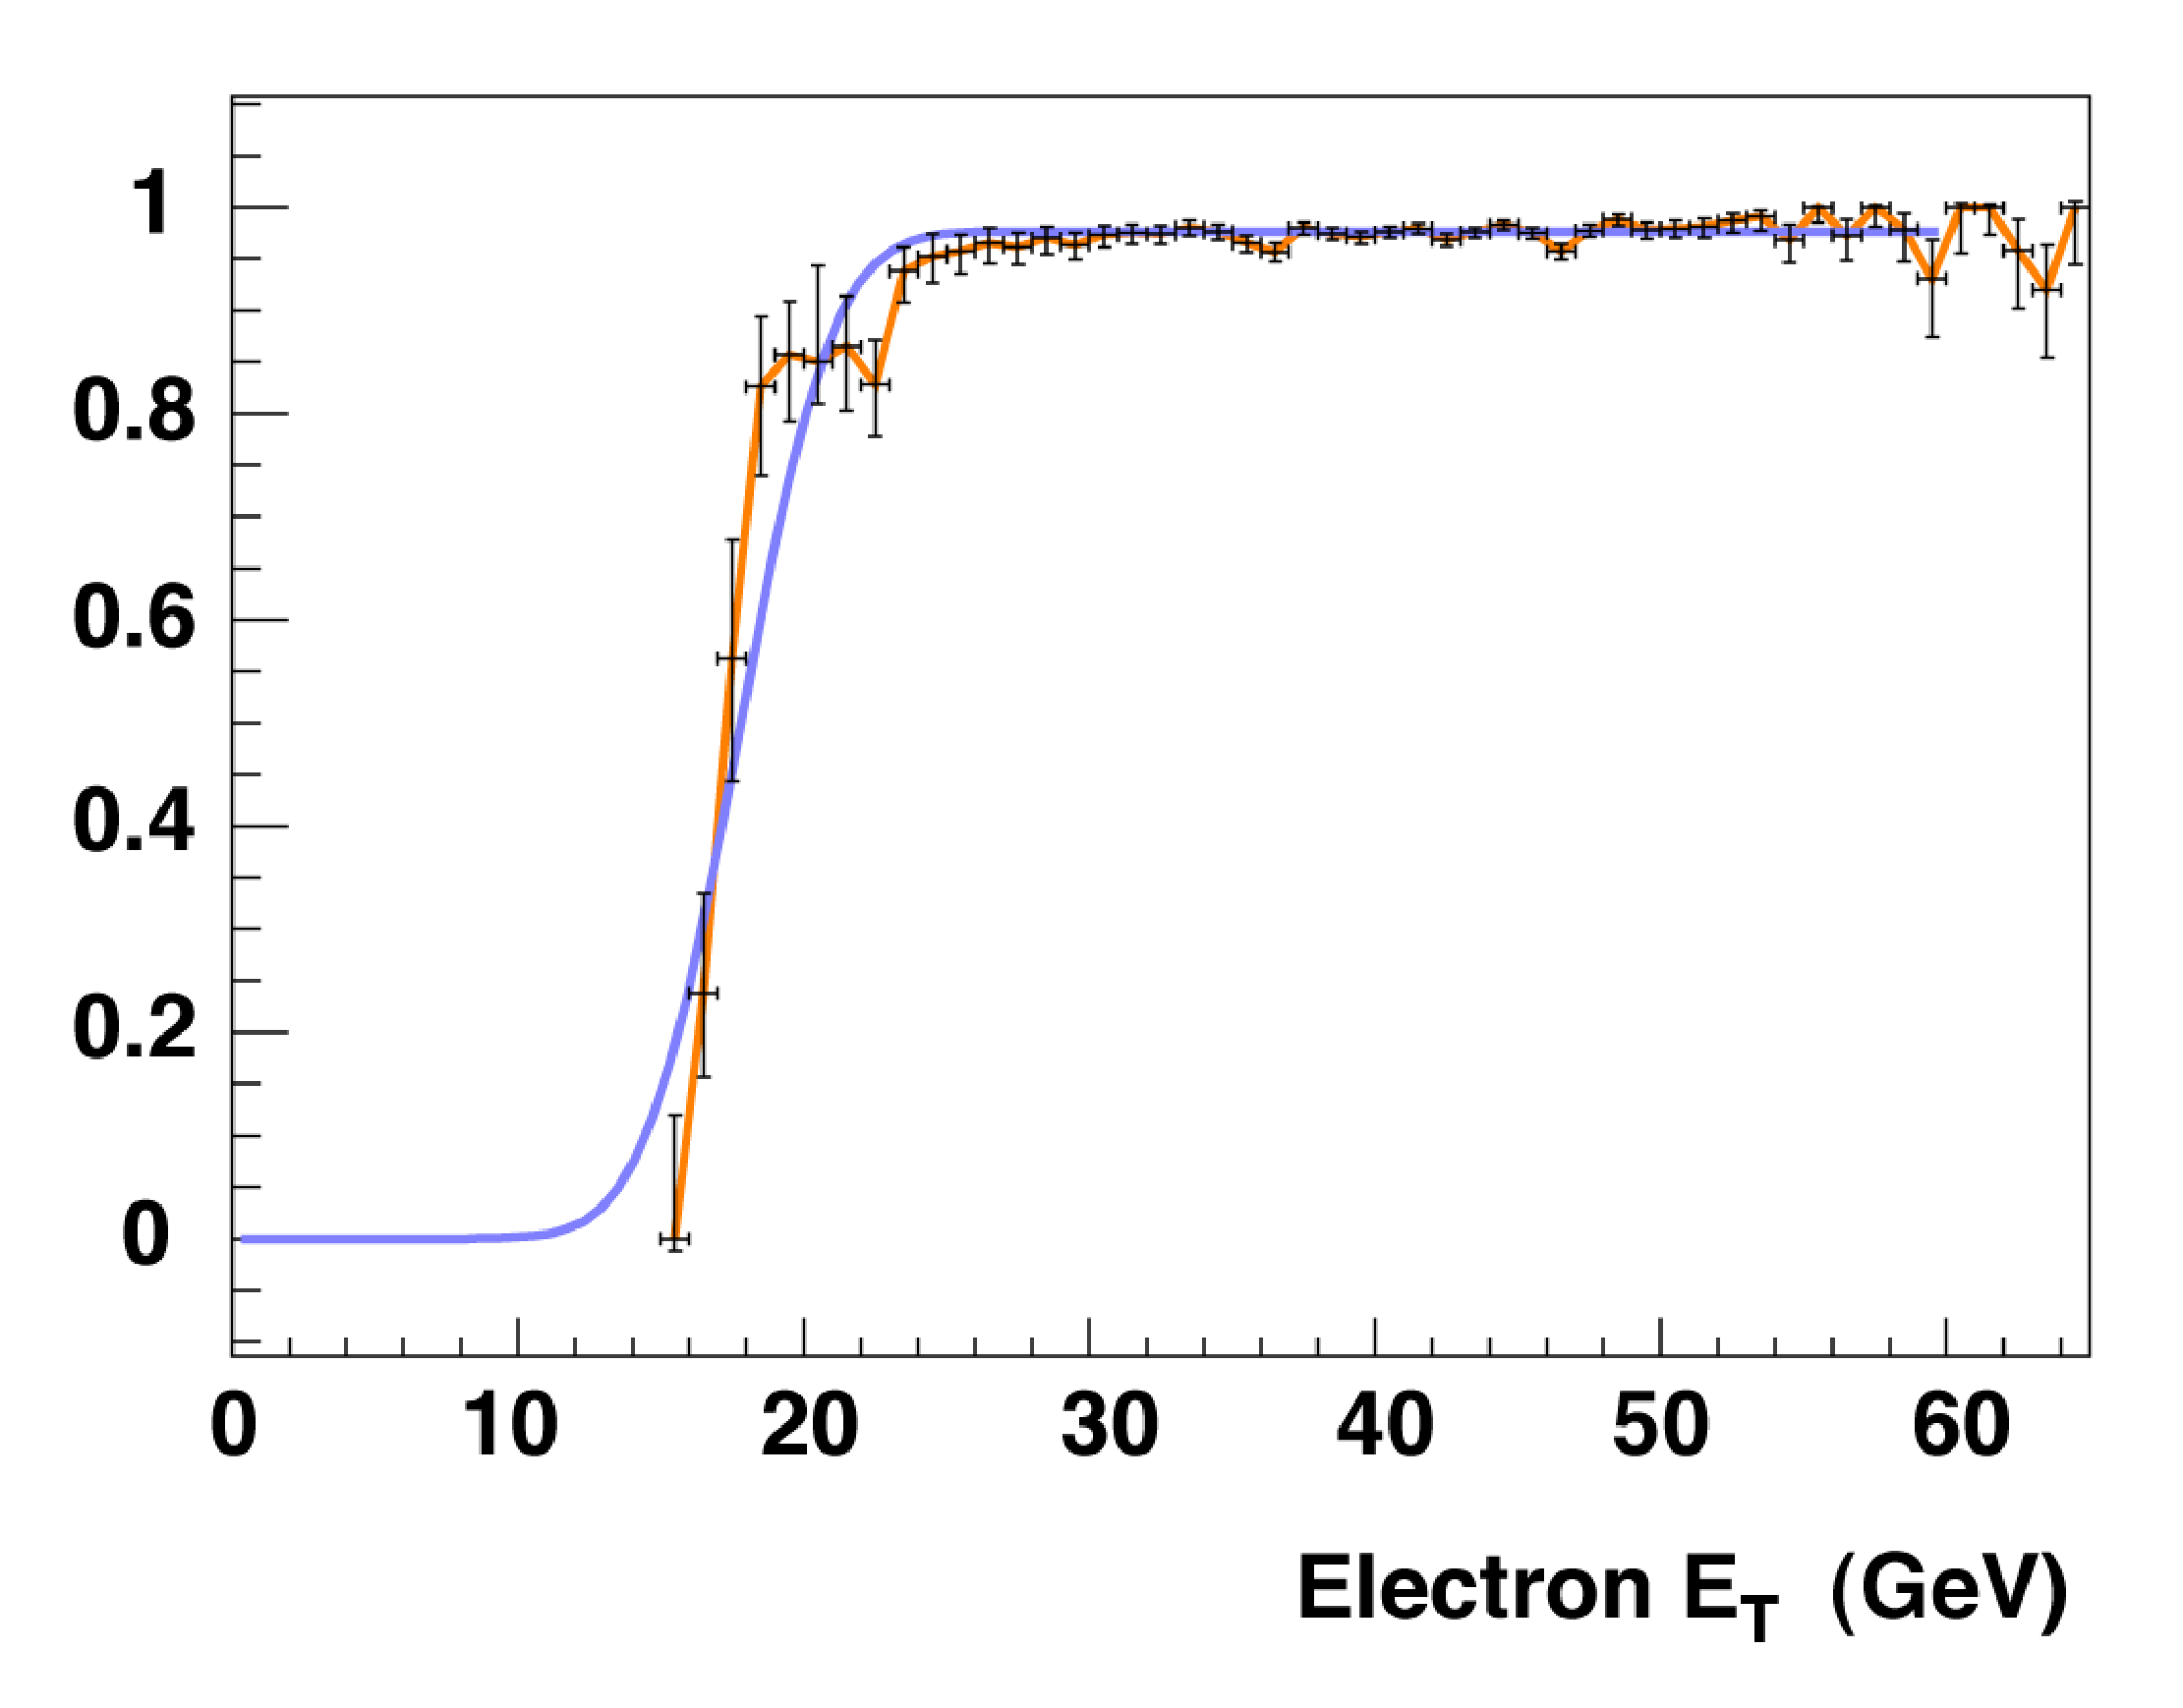
\includegraphics[width=0.35\textwidth]
{figures/electron_turn-on_curve_pt.eps}
\hspace{0.5in}
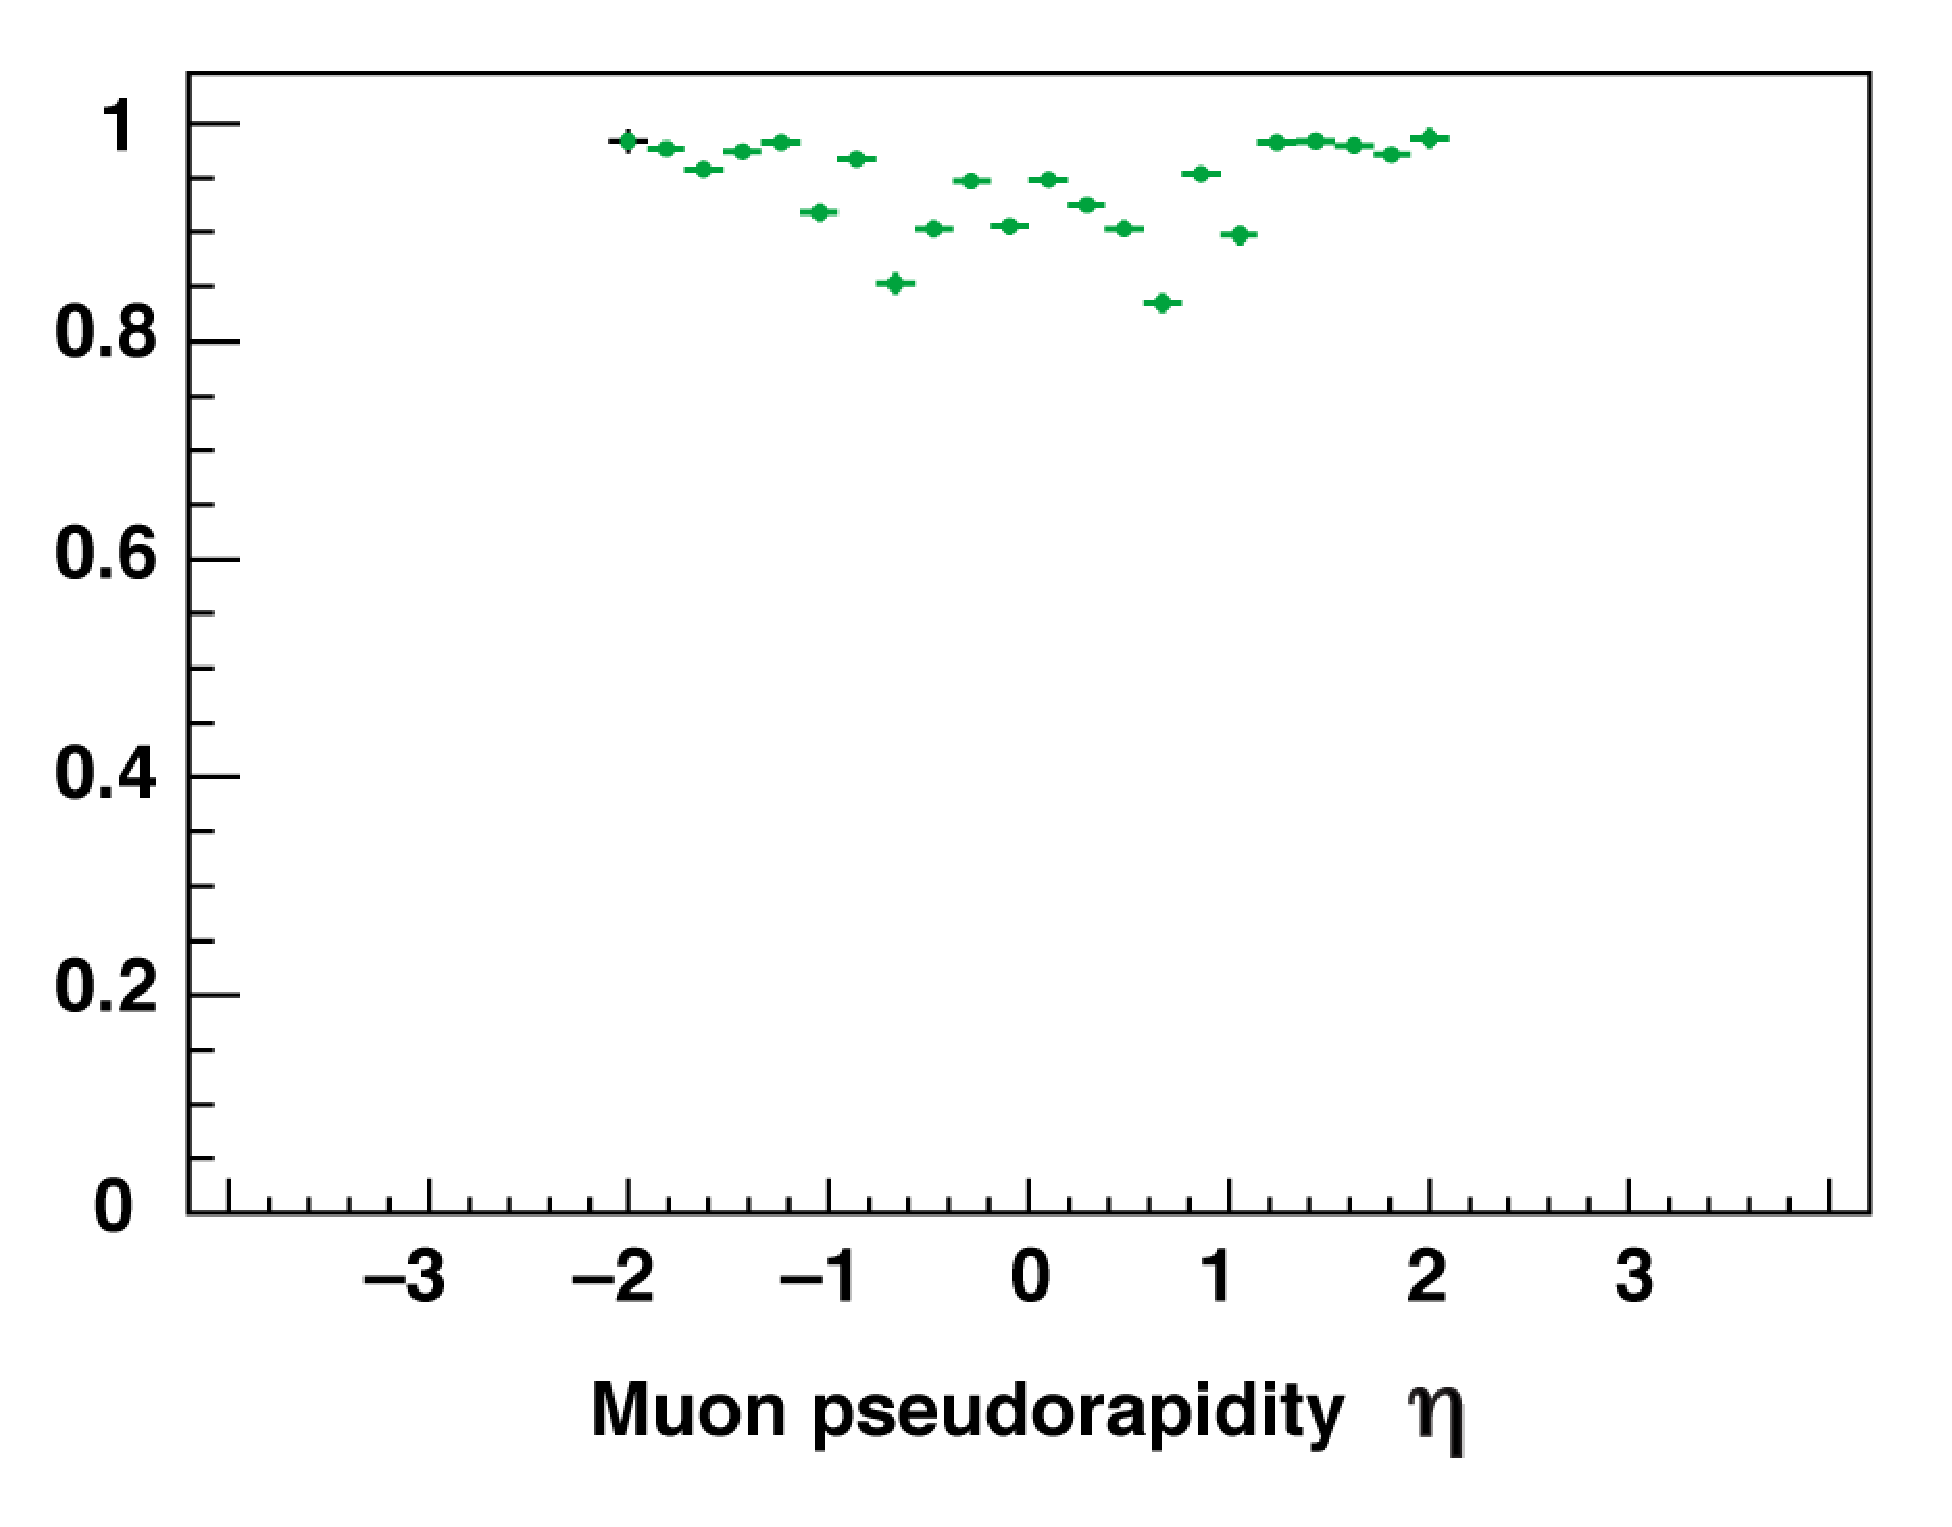
\includegraphics[width=0.35\textwidth]
{figures/muon_turn-on_curve_eta.eps}
\end{center}
\vspace{-0.1in}
\begin{minipage}{5.5in}
\caption[triggerturnons]{An example electron turn-on curve measured
as a function of the electron $p_T$ from trigger list v14 (left) and
an example muon turn-on curve measured as a function of {\deta} for
trigger lists v13--v15 (right). The muon curve is for Level 1 trigger
term mu1ptxatlx. The points are trigger efficiencies derived from data
in that bin (with uncertainty bars). The line is the corresponding fit
(for illustration purpose).}
\label{trigger-turnons}
\end{minipage}
\end{figure}

This analysis uses the ``caf\_trigger"~\cite{caf_trigger} package to
apply these turn-on curves to MC events. The caf\_trigger program
reads in turn-on curves for the number of physics objects (electrons,
muons, jets) in each event and the trigger list versions with the
associated integrated luminosities. It then uses ``processors'' to
perform combinatorics calculations and it then calculates the trigger
firing probabilities. Finally, it outputs a histogram of event
weights. The average efficiencies of $e$+jets and $\mu$+jets triggers
for signal events that pass selection are listed in
Tables~\ref{eltrigger-efficiencies} and
\ref{mutrigger-efficiencies}. These numbers are given for illustrative
purposes and are not used in the analysis.

\begin{table}[!h!tbp]
\begin{center}
\begin{minipage}{2.8in}
\begin{ruledtabular}
\begin{tabular}{c||cc} 
\multicolumn{3}{c}{\hspace{0.1in}\underline{Average Trigger Efficiencies}}\\
\multicolumn{3}{c}{\hspace{0.1in}\underline{in the Electron Channel}}\\
~~~ Trigger Version ~~~& $tb{\rar}e$+jets & $tqb{\rar}e$+jets \\
\hline
 v8.0 -- v9.0   &  92\%  &  92\%  \\            
 v9.0 -- v10.0  &  91\%  &  91\%  \\            
v10.0 -- v11.0  &  91\%  &  91\%  \\            
v11.0 -- v12.0  &  91\%  &  91\%  \\            
v12.0 -- v13.0  &  86\%  &  85\%  \\ 
v13.0 -- v13.3  &  87\%  &  86\%  \\            
v13.3 -- v14.0  &  86\%  &  85\%  \\         
v14.0 -- v15.0  &  88\%  &  87\%  \\
\hline		                
Overall average &  87\%  &  86\%
\end{tabular}
\end{ruledtabular}
\vspace{-0.1in}
\caption[eltriggerefficiencies]{Average electron-channel trigger
efficiencies for the single top events after selection.}
\label{eltrigger-efficiencies}
\end{minipage}
\end{center}
\end{table}


\begin{table}[!h!tbp]
\begin{center}
\begin{minipage}{2.8in}
\begin{ruledtabular}
\begin{tabular}{c||cc} 
\multicolumn{3}{c}{\hspace{0.1in}\underline{Average Trigger Efficiencies}}\\
\multicolumn{3}{c}{\hspace{0.1in}\underline{in the Muon Channel}}\\
~~~ Trigger Version ~~~& $tb{\rar}\mu$+jets & $tqb{\rar}\mu$+jets \\
\hline
 v8.0 -- v9.0   &  96\%  &  94\%  \\            
 v9.0 -- v10.0  &  93\%  &  90\%  \\            
v10.0 -- v11.0  &  91\%  &  88\%  \\            
v11.0 -- v12.0  &  92\%  &  88\%  \\            
v12.0 -- v13.0  &  91\%  &  88\%  \\ 
v13.0 -- v13.2  &  91\%  &  87\%  \\            
v13.2 -- v13.3  &  91\%  &  87\%  \\         
v13.3 -- v14.0  &  86\%  &  81\%  \\ 
v14.0 -- v14.2  &  92\%  &  89\%  \\   
v14.2 -- v14.3  &  92\%  &  89\%  \\
v14.3 -- v15.0  &  80\%  &  72\%  \\
\hline		                
Overall average &  87\%  &  82\%
\end{tabular}
\end{ruledtabular}
\vspace{-0.1in}
\caption[mutriggerefficiencies]{Average muon-channel trigger
efficiencies for the single top events after selection.}
\label{mutrigger-efficiencies}
\end{minipage}
\end{center}
\end{table}

\vspace{2in}

%---------------------------------------------------------------------
%---------------------------------------------------------------------
%% Lepton isolation efficiencies            # 2
\clearpage
%---------------------------------------------------------------------
%  Writeup of the improved search of Run II data for single top quark
%  production at DZero.
%  Started: Oct 2006
%  Authors: The Single Top Working Group
%---------------------------------------------------------------------
%

\appendix
\section*{Appendix 2 --- Lepton Isolation Probabilities}
\label{epsilons}

Normalization of the $W$+jets and multijet backgrounds to data is
performed using the matrix method as explained in
Section~\ref{matrix-method}. To determine the separate contributions
from signal-like real-lepton events and background fake-lepton events
in our data, we rely on the measurement of two probabilities,
$\varepsilon_{{\rm real-}\ell}$ and $\varepsilon_{{\rm fake-}\ell}$.

$\varepsilon_{{\rm real-}\ell}$ is the probability for a real lepton
to pass the isolation requirements. It is obtained using a $Z{\rar}
ee$ sample for the electrons and $Z {\rar} \mu\mu$ sample for the
muons. One of the leptons is ``tagged'' as \emph{tight}, then the
$\varepsilon_{{\rm real-}\ell}$ is calculated measuring the
probability of the other ``probe'' lepton to pass the
\emph{tight} selection cut.

The $\pt$ and $\eta$ dependence for the electron case is shown in
Fig.~\ref{cc-eps-signal}. The $\pt$ and jet multiplicity dependence in
the muon case is shown in Fig.~\ref{mu-eps-signal}. The average values
for $\varepsilon_{{\rm fake-}e}$ and $\varepsilon_{{\rm fake-}\mu}$ as
a function of the jet multiplicity are given in
Table~\ref{eps-signal}. The overall uncertainty for $\varepsilon_{{\rm
fake-}\ell}$ is $1\%$ statistical and $2\%$ systematic.

\vspace{-0.1in}
\begin{figure}[!h!tbp]
\includegraphics[width=0.34\textwidth]
{figures/eps_sig_el_pt.eps}
\hspace{0.5in}
\includegraphics[width=0.34\textwidth]
{figures/eps_sig_el_eta.eps}
\vspace{-0.1in}
\caption[ccepssignal]{Transverse momentum and detector
pseudorapidity dependence of $\varepsilon_{{\rm real-}e}$.}
\label{cc-eps-signal}
\end{figure} 

\vspace{-0.3in}
\begin{figure}[!h!tbp]
\includegraphics[width=0.36\textwidth]
{figures/eps_sig_mu_pt.eps}
\hspace{0.5in}
\includegraphics[width=0.36\textwidth]
{figures/eps_sig_mu_njets.eps}
\vspace{-0.1in}
\caption[muepssignal]{Transverse momentum and jet
multiplicity dependence of $\varepsilon_{{\rm real-}\mu}$.}
\label{mu-eps-signal}
\end{figure}

\vspace{-0.2in}
\begin{table}[!h!tbp]
\begin{center}
\begin{minipage}{2.5 in}
\begin{ruledtabular}
\begin{tabular}{c||cc}
\multicolumn{3}{c}{\underline{Real-Lepton Probabilities}}
\vspace{0.1in}\\
No. of jets & $\varepsilon_{{\rm real-}e}$
            & $\varepsilon_{{\rm real-}\mu}$ \\
\hline
  1  &  $(87.3 \pm 2.1)\%$  &  $(99.1 \pm 2.2)\%$  \\
  2  &  $(87.4 \pm 2.1)\%$  &  $(98.9 \pm 2.2)\%$  \\
  3  &  $(87.4 \pm 2.1)\%$  &  $(98.7 \pm 2.2)\%$  \\
  4  &  $(87.5 \pm 2.1)\%$  &  $(96.1 \pm 2.1)\%$
\end{tabular}
\end{ruledtabular}
\vspace{-0.1in}
\caption[epssignal]{Average values for $\varepsilon_{{\rm real-}\ell}$
in the electron and muon samples for different jet multiplicities.}
\label{eps-signal}
\end{minipage}
\end{center}
\end{table}

\vspace{-0.2in}
$\varepsilon_{{\rm fake-}\ell}$ is the probability for a fake lepton
to pass the isolation requirements. It is obtained using a data
sample. Assuming that the low $\met$ region ($\met < 10$~GeV) is
dominated by the multijet background, and that $\varepsilon_{{\rm
fake-}\ell}$ is independent of the $\met$ cut, then $\varepsilon_{{\rm
fake-}\ell}$ is determined as the ratio of \emph{tight} over
\emph{loose} events in the low $\met$ region.
We studied $\varepsilon_{{\rm fake-}e}$ as a function of several
parameters, finding no dependence on the lepton $\pt$ or lepton
$\eta$, but dependence on the trigger version (because the isolation
requirement in the trigger changed) and jet multiplicity. For
$\varepsilon_{{\rm fake-}\mu}$, we performed a similar set of studies
and found no need to parametrize as a function of the trigger version
as the muon isolation in the trigger did not change during this
period. However, we did paramterize as a function of the muon
pseudorapidity where there is a small dependence. Although there is
also dependence on muon transverse momentum, parametrizing in this as
well does not change the overall result, so we have not done this.
Figure~\ref{fig:eps-qcd-e} show the calculation of $\varepsilon_{{\rm
fake-}e}$ from the ratio of tight to loose events as a function of
{\met} for each jet multiplicity, with all trigger versions
combined. Figure~\ref{fig:eps-qcd-mu} shows $\varepsilon_{{\rm
fake-}\mu}$ as a function of the muon pseudorapidity. A summary of the
results is presented in Table~\ref{eps-qcd}.

\begin{figure}[!h!tbp]
\includegraphics[width=0.98\textwidth]
{figures/eps_qcd_el_alltrigs_met}
\vspace{-0.1in}
\caption[figepsqcde]{$\varepsilon_{{\rm fake}e}$ calculated in
the $0 < {\met} < 10$ GeV region of the distributions of tight/loose
events, with all trigger versions combined.}
\label{fig:eps-qcd-e}
\end{figure}

\begin{figure}[!h!tbp]
\includegraphics[width=0.98\textwidth]
{figures/eps_qcd_mu_eta}
\vspace{-0.1in}
\caption[figepsqcdmu]{$\varepsilon_{{\rm fake}\mu}$ as a function of
the muon pseudorapidity.}
\label{fig:eps-qcd-mu}
\end{figure}

\begin{table}[!h!tbp]
\begin{center}
\begin{minipage}{6.5 in}
\begin{ruledtabular}
\begin{tabular}{c||ccccc|c}
\multicolumn{7}{c}{\hspace{0.8in}\underline{Fake-Lepton Probabilities}}
\vspace{0.05in}\\
& \multicolumn{5}{c|}{ $\varepsilon_{{\rm fake-}e}$, Trigger Version} & \\
No. of jets & v8--v11   &     v12     &     v13a    &     v13b    &     v14     &     $\varepsilon_{{\rm fake-}\mu}$ \\
\hline 
 1 & $(11.2 \pm 0.5)\%$ & $(17.9 \pm 0.6)\%$ & $(18.7 \pm 1.2)\%$ & $(19.1 \pm 0.6)\%$ & $(18.5 \pm 0.6)\%$ & $40.8\%$ \\
 2 & $(12.8 \pm 1.0)\%$ & $(19.2 \pm 1.0)\%$ & $(18.8 \pm 2.2)\%$ & $(19.4 \pm 1.1)\%$ & $(22.0 \pm 1.2)\%$ & $35.8\%$ \\
 3 & $(13.6 \pm 1.5)\%$ & $(19.5 \pm 1.6)\%$ & $(19.8 \pm 3.4)\%$ & $(19.2 \pm 1.6)\%$ & $(19.4 \pm 1.7)\%$ & $34.2\%$ \\
 4 & $(10.0 \pm 2.8)\%$ & $(15.5 \pm 2.9)\%$ & $(20.9 \pm 8.6)\%$ & $(17.7 \pm 3.3)\%$ & $(20.7 \pm 3.7)\%$ & $30.9\%$
\end{tabular}
\end{ruledtabular}
\vspace{-0.1in}
\caption[epsqcd]{$\varepsilon_{{\rm fake-}e}$ as a function of
the trigger version and jet multiplicity, and $\varepsilon_{{\rm
fake-}\mu}$ averaged over $\eta$.}
\label{eps-qcd}
\end{minipage}
\end{center}
\end{table}

\clearpage

%---------------------------------------------------------------------
%---------------------------------------------------------------------
%% Ratio of Wbb and Wcc to Wjj              # 3
\clearpage
%---------------------------------------------------------------------
%  Writeup of the improved search of Run II data for single top quark
%  production at DZero.
%  Started: Oct 2006
%  Authors: The Single Top Working Group
%---------------------------------------------------------------------
%
\appendix
\section*{Appendix 3 --- Scaling the $W$+Jets Heavy Flavor Fraction}
\label{appendix-wjets-scaling}

The {\sc alpgen} leading order cross section calculations for
$Wb\bar{b}$, $Wc\bar{c}$, and $Wjj$ have sizeable uncertainties and
are very sensitive to the renormalization and factorization scales. In
previous analyses, we used MCFM~\cite{MCFM} with the same {\sc alpgen}
parton level cuts to estimate the NLO cross sections of $Wb\bar{b}$
and $Wjj$, set the relative fraction of $Wb\bar{b}$ and $Wjj$ based on
these numbers, and then normalized the overall $W$+jets sample to data
based on the matrix method results. That gave us the best estimate,
with uncertaintiess, of what fraction of events in the $W$+jets sample
had heavy flavor jets. With the new matched {\sc alpgen} samples, {\sc
alpgen} is actually run with no parton level cuts since the matching
scheme takes care of avoiding divergences by clustering partons into
parton-jets with certain cuts ($\pt>8$~GeV and $\Delta R>0.4$). For a
description of the matching scheme, and the details of our production
samples, see Ref.~\cite{FOMEcs}. Since MCFM and matched {\sc alpgen}
do not agree in the LO cross section, it is difficult to use the MCFM
NLO cross section to scale our {\sc alpgen} generated samples.

As done in previous analyses, we scale the total $W$+jets leading
order yield to data before $b$-tagging by means of the ``matrix
method,'' as explained in detail in Section~\ref{matrix-method}.
Table~\ref{mmwjets-factors} presents the scale factors from the matrix
method needed to make the LO {\alpgen} $W$+jets yields match the
data. This normalization is done for $Wb\bar{b}$, $Wc\bar{c}$, and
$Wjj$ altogether.

\vspace{0.05in}
\begin{table}[!h!tbp]
\begin{center}
\begin{minipage}{3.5 in}
\begin{ruledtabular}
\begin{tabular}{l||cccc}
\multicolumn{5}{c}{\hspace{0.4in}\underline{$W$+jets Matrix Method Normalization}}\vspace{0.1in} \\
                 &  1 jet  &  2 jets &  3 jets &  4 jets  \\
\hline
Electron channel &   1.39  &   1.42  &   1.14  &   0.88   \\
Muon channel     &   1.55  &   1.66  &   1.50  &   1.16
\end{tabular}
\end{ruledtabular}
\vspace{-0.1 in}
\caption[mmwjetsfactors]{Scale factors applied to the LO $W$+jets
samples, to match the data from the matrix method normalization.}
\label{mmwjets-factors}
\end{minipage}
\end{center}
\end{table}

Once the overall normalization to data is performed, we still need to
correct the relative composition of $Wb\bar{b}$ and $Wc\bar{c}$ with
respect to $Wjj$. We assume the same ratio applies for $Wb\bar{b}$ and
$Wc\bar{c}$. We have used our data to measure this heavy flavor ratio
in the form of a scale factor $\alpha$ such that:
$$
\alpha(Wb\bar{b}+Wc\bar{c})+Wjj+\ttbar+{\rm QCD = Data,}
$$ where $Wb\bar{b}$ and $Wc\bar{c}$ are the yields as given by the
{\alpgen} cross section. However, we should not normalize the
background to the data in the signal region, so we have chosen a
factor 1.5, and assigned a 30\% uncertainty to it, based on the
results shown in Table~\ref{alpha-factors} for the zero-tag case. The
one-jet bin can also be utilized to derive $\alpha$ but the result is
more difficult to generalize to the signal region. The zero-tag sample
is not used for the measurement, has ample statistics, and shows very
similar sensitivity to the heavy flavor ratio as the signal
region. The zero-tag sample contains about 10\% (20\%) $Wc\bar{c}$ in
the 1jet (2jet) bin. The $Wb\bar{b}$ fraction here is much
smaller. But the sum of $Wc\bar{c} + Wb\bar{b}$ is large enough to be
able to measure the relative heavy flavor scale factor.

\clearpage

\begin{table}[!h!tbp]
\begin{center}
\begin{minipage}{4.5 in}
\begin{ruledtabular}
\begin{tabular}{l||cccc}
\multicolumn{5}{c} {\hspace{0.5in}\underline{Scale Factor $\alpha$ to Match Heavy Flavor Fraction to Data}}\vspace{0.1in} \\
                 &     1 jet      &      2 jets     &      3 jets     &       4 jets     \\
\hline
% these numbers are Yann's alphas, but multiplied by 1.5, so they should be close to 1.5:
Electron Channel  &                 &                 &                 &                  \\
~~0 tags          & 1.53 $\pm$ 0.10 & 1.48 $\pm$ 0.10 & 1.50 $\pm$ 0.20 &  1.72 $\pm$ 0.40 \\
~~1 tag           & 1.29 $\pm$ 0.10 & 1.58 $\pm$ 0.10 & 1.40 $\pm$ 0.20 &  0.69 $\pm$ 0.60 \\
~~2 tags          &       ---       & 1.71 $\pm$ 0.40 & 2.92 $\pm$ 1.20 & -2.91 $\pm$ 3.50 \\
Muon Channel      &                 &                 &                 &                  \\
~~0 tags          & 1.54 $\pm$ 0.10 & 1.50 $\pm$ 0.10 & 1.52 $\pm$ 0.10 &  1.38 $\pm$ 0.20 \\
~~1 tag           & 1.11 $\pm$ 0.10 & 1.52 $\pm$ 0.10 & 1.32 $\pm$ 0.20 &  1.86 $\pm$ 0.50 \\
~~2 tags          &       ---       & 1.40 $\pm$ 0.40 & 2.46 $\pm$ 0.90 &  3.78 $\pm$ 2.80
% These numbers are the alphas (when 1.5 is applied), so they should be close to 1
%$\mu$+jets 0 tag & 1.03 $\pm$ 0.1 & 1.00 $\pm$ 0.1&  1.01 $\pm$ 0.1 & 0.92 $\pm$ 0.2 \\
%$\mu$+jets 1 tag & 0.74 $\pm$ 0.1 & 1.01 $\pm$ 0.1&  0.88 $\pm$ 0.2 & 1.24 $\pm$ 0.5 \\
%$\mu$+jets 2 tag & ---            & 0.93 $\pm$ 0.4&  1.64 $\pm$ 0.9 & 2.52 $\pm$ 2.8 \\ \hline
%$e$+jets 0 tag   & 1.02 $\pm$ 0.1 & 0.99 $\pm$ 0.1&  1.00 $\pm$ 0.2 & 1.15 $\pm$ 0.4 \\
%$e$+jets 1 tag   & 0.86 $\pm$ 0.1 & 1.05 $\pm$ 0.1&  0.93 $\pm$ 0.2 & 0.46 $\pm$ 0.6 \\
%$e$+jets 2 tag   & ---            & 1.14 $\pm$ 0.4&  1.95 $\pm$ 1.2 &-1.94 $\pm$ 3.5 \\
\end{tabular}
\end{ruledtabular}
\vspace{-0.1 in}
\caption[alphafactors]{Scale factor $\alpha$ for the $Wb\bar{b}$ and
$Wc\bar{c}$ yields to match the data in each jet bin, for 0 tag, 1
tag, and 2 tag samples. The uncertainties are statistical only.}
\label{alpha-factors}
\end{minipage}
\end{center}
\end{table}

% (The following may well be true, but let's not promise it
% publically in case we do not have time to do it!)
%
% We intend to cross check this scaling and its uncertainty by
% measuring the same $\alpha$ factor in our signal region using a
% sample with low discriminant output value from the multivariate
% analysis that will not be used in the final measurement.

Figure~\ref{fig:alphaseqzerotag} shows graphically the values of
$\alpha$ in the zero tag sample for electrons and muons in each jet
bin (eight numbers in total).

\begin{figure}[!h!tbp]
\includegraphics[width=0.6\textwidth]
{figures/alpha-from-eqzerotag-sample}
\vspace{-0.1in}
\begin{minipage}{4in}
\caption[tag]{The values of $\alpha$ in the zero tag sample for
electron and muon channel in each jet multiplicity. The eight values
can be read in Table.~\ref{alpha-factors}.}
\label{fig:alphaseqzerotag}
\end{minipage}
\end{figure}


%---------------------------------------------------------------------
%---------------------------------------------------------------------
%% All about b tagging                      # 4
\clearpage
%---------------------------------------------------------------------
%  Writeup of the improved search of Run II data for single top quark
%  production at DZero.
%  Started: Oct 2006
%  Authors: The Single Top Working Group
%---------------------------------------------------------------------
%
\appendix
\section*{Appendix 4 --- Neural Network $B$-Tagging}
\label{appendix-nn-btagging}

We are using the neural network $b$-tagging algorithm version 1.1 from
the B-ID Agorithm Group. We present here an explanation of how we
apply this algorithm to Monte Carlo events. For data events, the
algorithm is applied directly.

\subsection{Taggability}
\label{taggability}

Taggability is defined as the probability that a jet is taggable,
where this means that a calorimeter jet is matched within $\Delta R <
0.5$ of a track jet, the track jet consists of at least two tracks,
with $\Delta R < 0.5$ between them, and the tracks used to form the
track jet have at least one SMT hit on them and at least one of the
tracks has $p_T > 1$~GeV.

Because our model of the detector does not completely match the real
one, we cannot apply the taggability requirements to Monte Carlo jets
directly and get the same answer as for data. We compensate for this
by instead applying taggability rate functions to the MC events.
These functions are parametrized in jet $\pt$, jet $\eta$ and primary
vertex $z$. They have been derived on the single top loose data
samples, where the isolation of the lepton is only required to be
loose (that is, all preselection except the tight lepton isolation) to
keep enough statistics for the measurement. Since these functions are
applied to tight samples, cross checks have been made to validate
their applicability. The observed taggability is measured (making the
jet selection for the jet to be taggable) on the tight data sample and
compared with the taggability rate function value in the same tight
data events. The results can be seen in
Fig.~\ref{fig:taggvalidation}. The observed taggability and the
predicted taggability give the same result within uncertainties.

\begin{figure}[!h!tbp]
\begin{center}
\includegraphics[width=0.49\textwidth]
{figures/taggability_el_validation.eps}
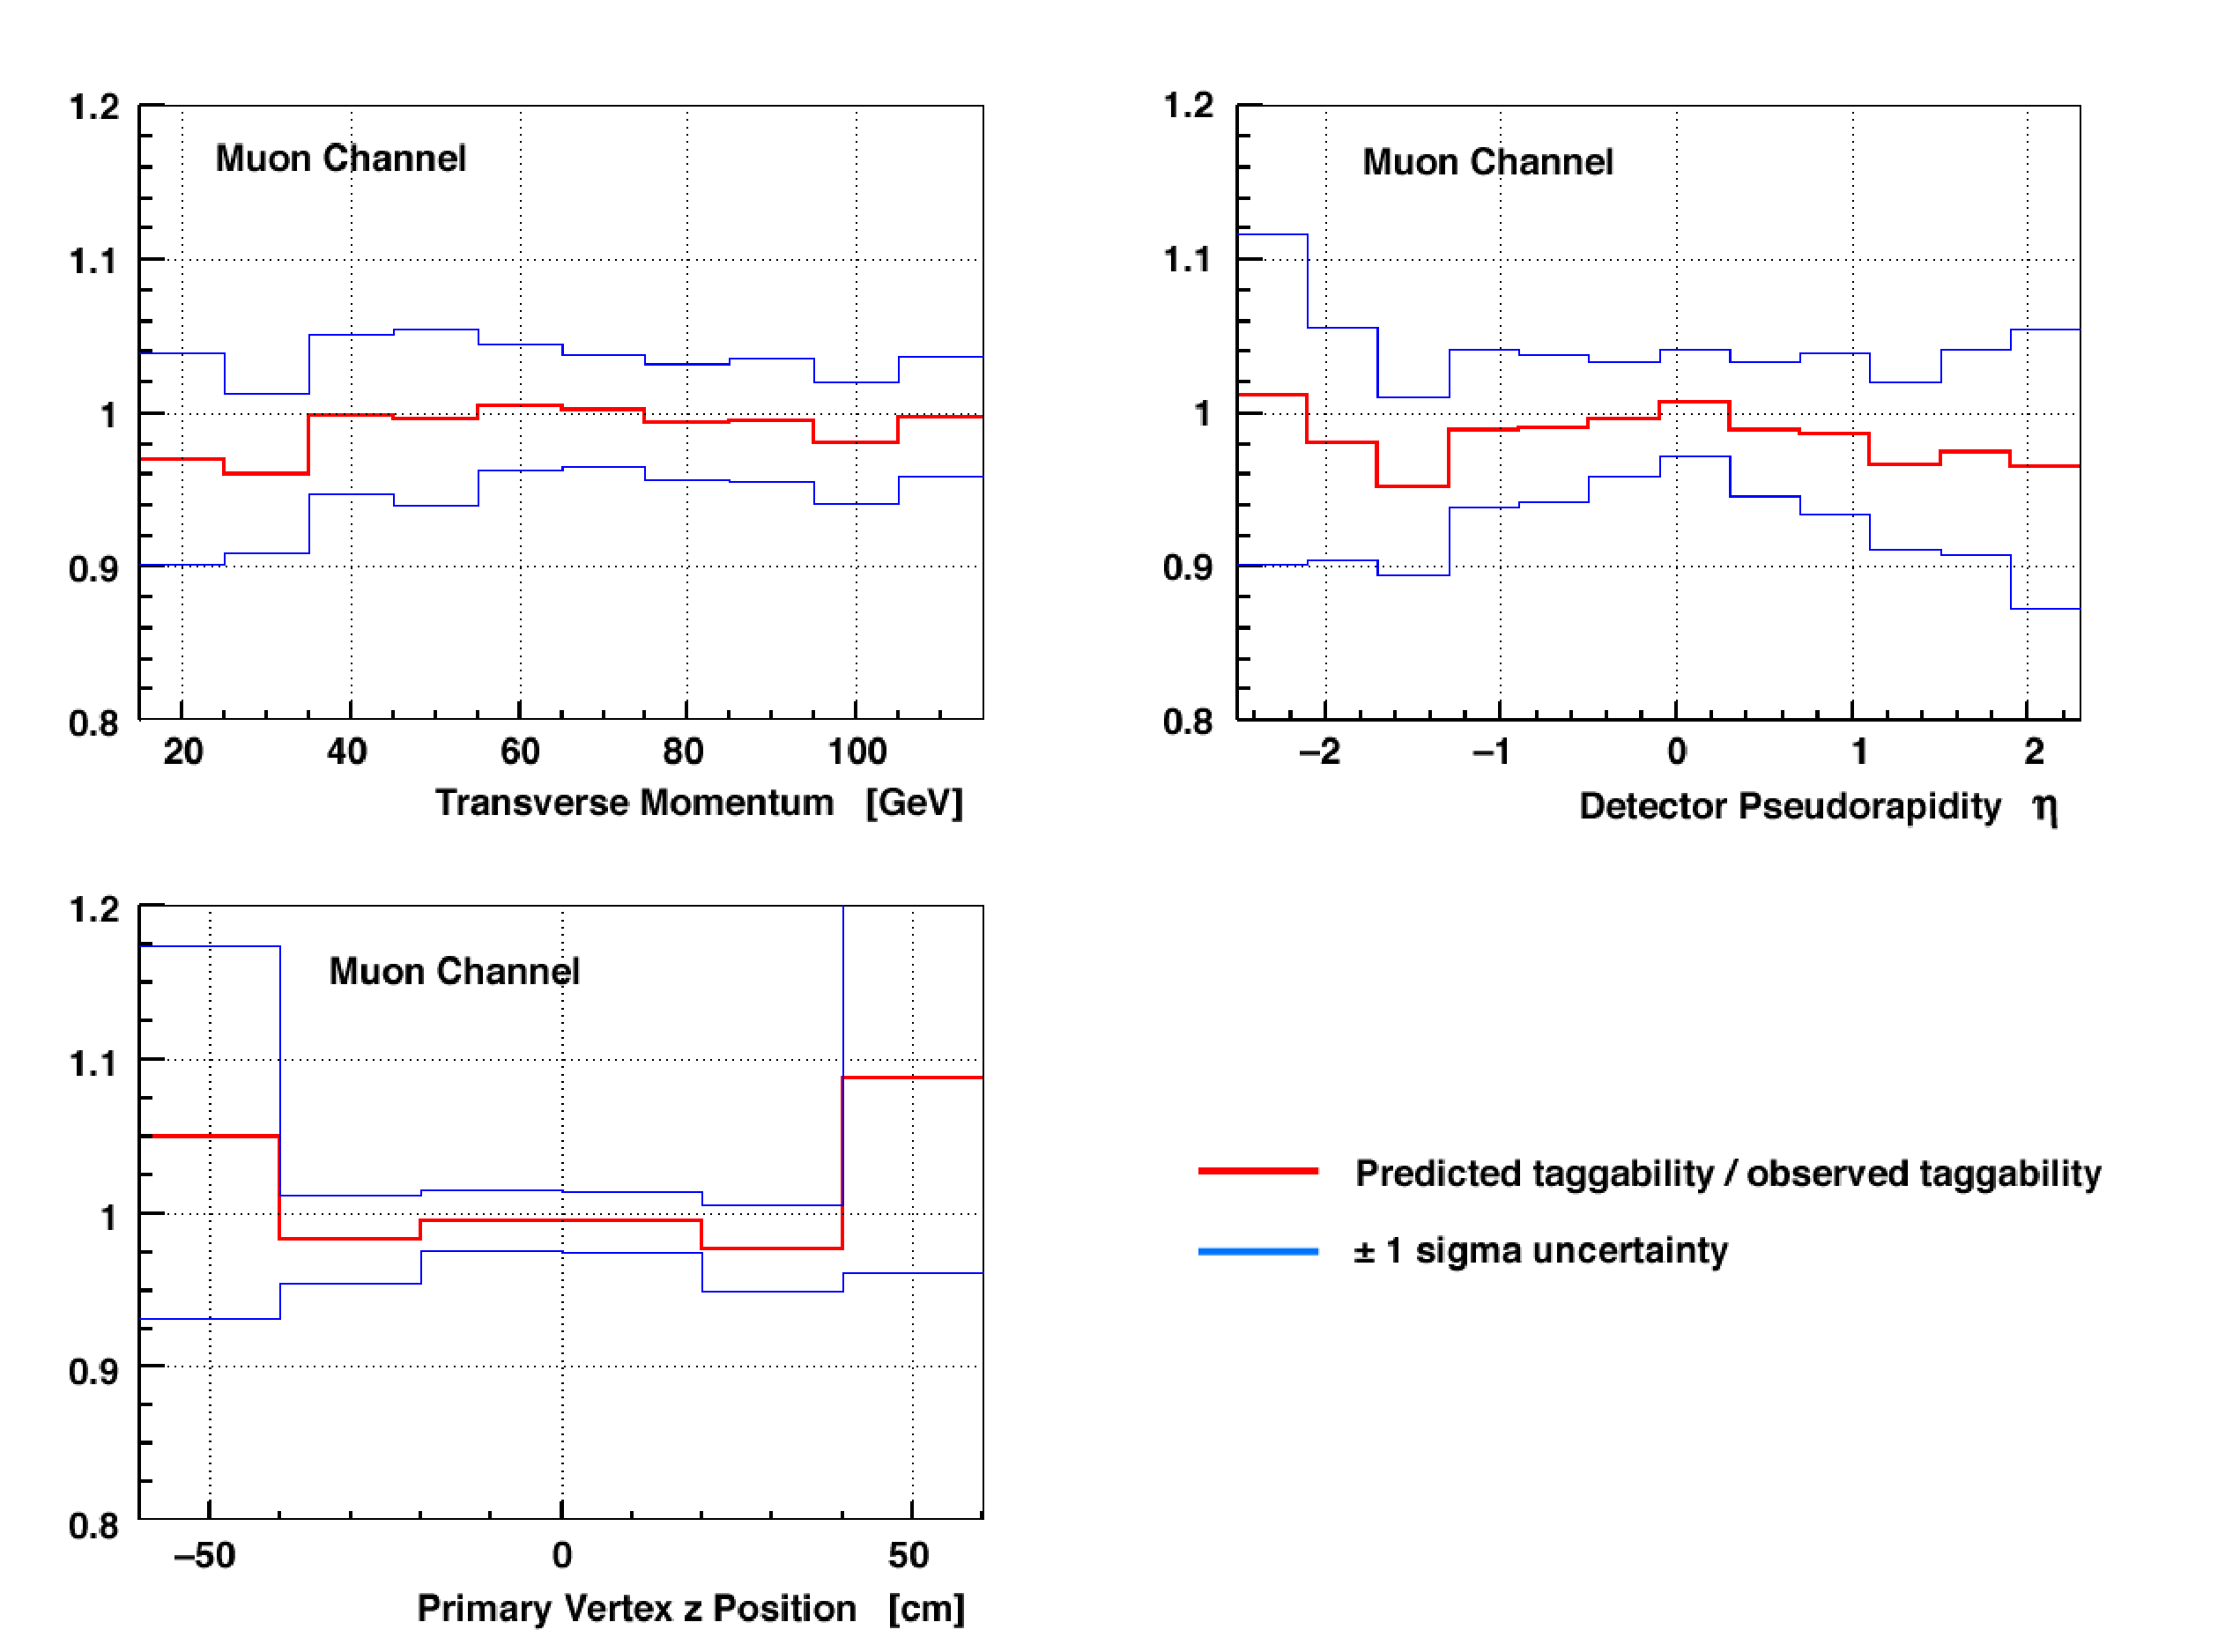
\includegraphics[width=0.49\textwidth]
{figures/taggability_mu_validation.eps}
\end{center}
\vspace{-0.1in}
\caption[tag]{The ratio of the predicted taggability rate function
over the observed taggability on the electron channel (upper plots)
and muon channel (lower plots) tight data sample. The taggability rate
function is derived on the loose data sample, but it matches the
observed taggability in the tight sample.}
\label{fig:taggvalidation}
\end{figure}

\clearpage

\subsection{$b$-Tagging Efficiencies}
\label{trfs}

The $b$-jet efficiency is measured in data, using a muon-in-jet sample
(BID sample) and a $b$-enriched subset consisting of muonic jets with
an away-jet tag probability of JLIP$<0.5$. This semileptonic
efficiency is denoted as $\varepsilon^{\rm DATA}_{b\to\mu}$. If we
apply the NN tagger to an MC sample with an admixture of $Z\to
b\bar{b}$ and $\ttbar$ MC, where the $b$~jets are forced to contain a
muon inside them, we obtain the semileptonic MC efficiency:
$\varepsilon^{MC}_{b\to\mu}$. The difference in efficiency between a
simulated jet and a jet in the data is parametrized in a data/MC scale
factor as a function of jet $\pt$ and $\eta$:
\vspace{-0.1in}
$$
SF_{b} = \frac{\varepsilon^{\rm DATA}_{b\to\mu}}
{\varepsilon^{MC}_{b\to\mu}}.
$$

To obtain the inclusive $b$-decay efficiency in data
$\varepsilon_{b}$, which is what we need to apply in our MC samples,
we just use:
\vspace{-0.1in}
$$
\varepsilon_b = \varepsilon^{\rm MC}_b \times SF_{b},
$$
\noindent where $\varepsilon^{\rm MC}_b$ is the efficiency to tag a
$b$~jet in an MC sample containing inclusive decays of the $b$~quark.
By using this procedure, we obtain the topological dependence of the
$b$-tagging efficiency from $\ttbar$ and $Z\to b\bar{b}$ samples,
while the overall efficiency normalization is calibrated to
data. However, one of our main backgrounds, $Wb\bar{b}$, produces
$b$~quarks not from $t$ or $Z$ decays, but from gluon splitting and
thus has somewhat different kinematics. It has been studied that
$b$~quarks from gluon splitting carry a smaller fraction of the total
jet momentum than $b$~quarks from $t$ or $Z$ decays. This results in a
5--10\% overestimation of the $\varepsilon_b$ over the tagger applied
directly to the MC, for jets below 30~GeV. The uncertainty on the
$\varepsilon_b$ is set large enough to cover this effect in this
region.
% See: http://www-d0.hef.kun.nl//askArchive.php?base=agenda&categ=a061800&id=a061800s1t1/transparencies

To obtain the inclusive $c$-quark $\varepsilon_c$, we assume that
$SF_c = SF_b$ and measure $\varepsilon^{\rm MC}_c$ in a combined MC
$c$ sample (with $Z$, QCD and $\ttbar$ decays to $c$ quarks). The
measured $\varepsilon_b$ and $\varepsilon_c$ dependences are shown in
Fig.~\ref{fig:NNTRFs} together with the direct tagger efficiency.

\vspace{0.1in}
\begin{figure}[!h!tbp]
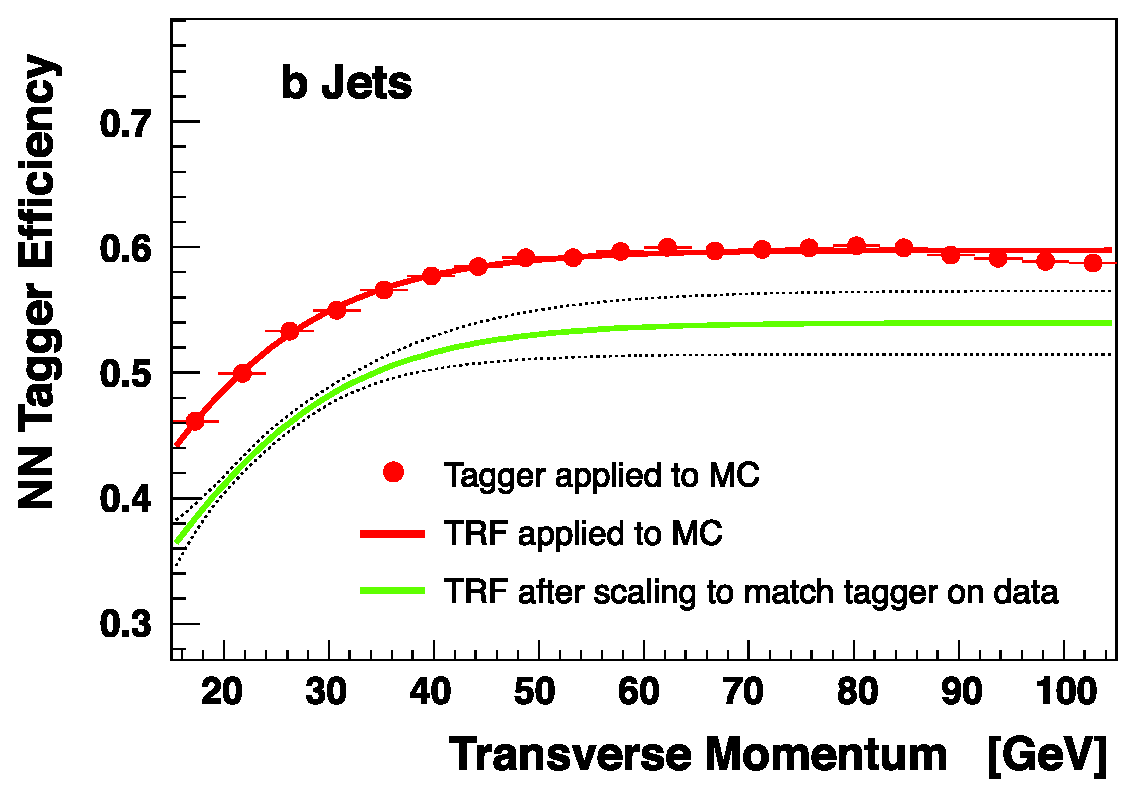
\includegraphics[width=0.32\textwidth]
{figures/TRF_b_pt.eps}
\hspace{0.5in}
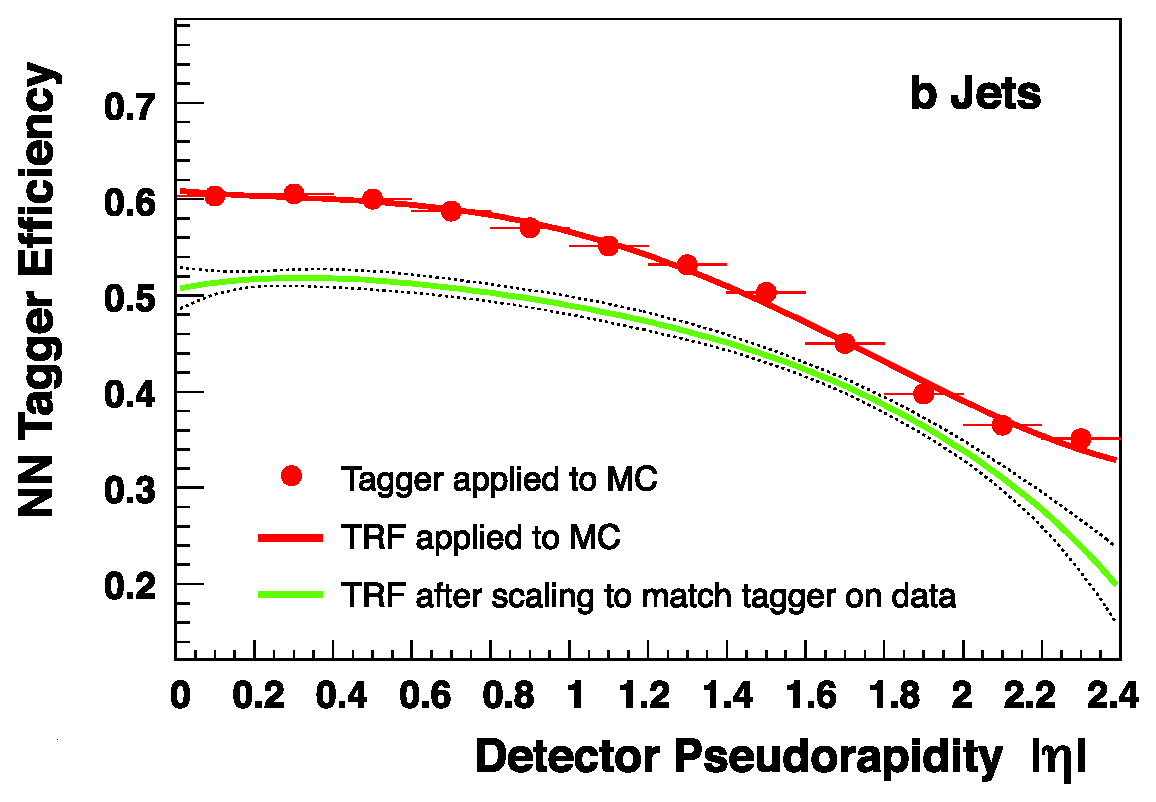
\includegraphics[width=0.32\textwidth]
{figures/TRF_b_eta.eps}
\hspace{0.1in}
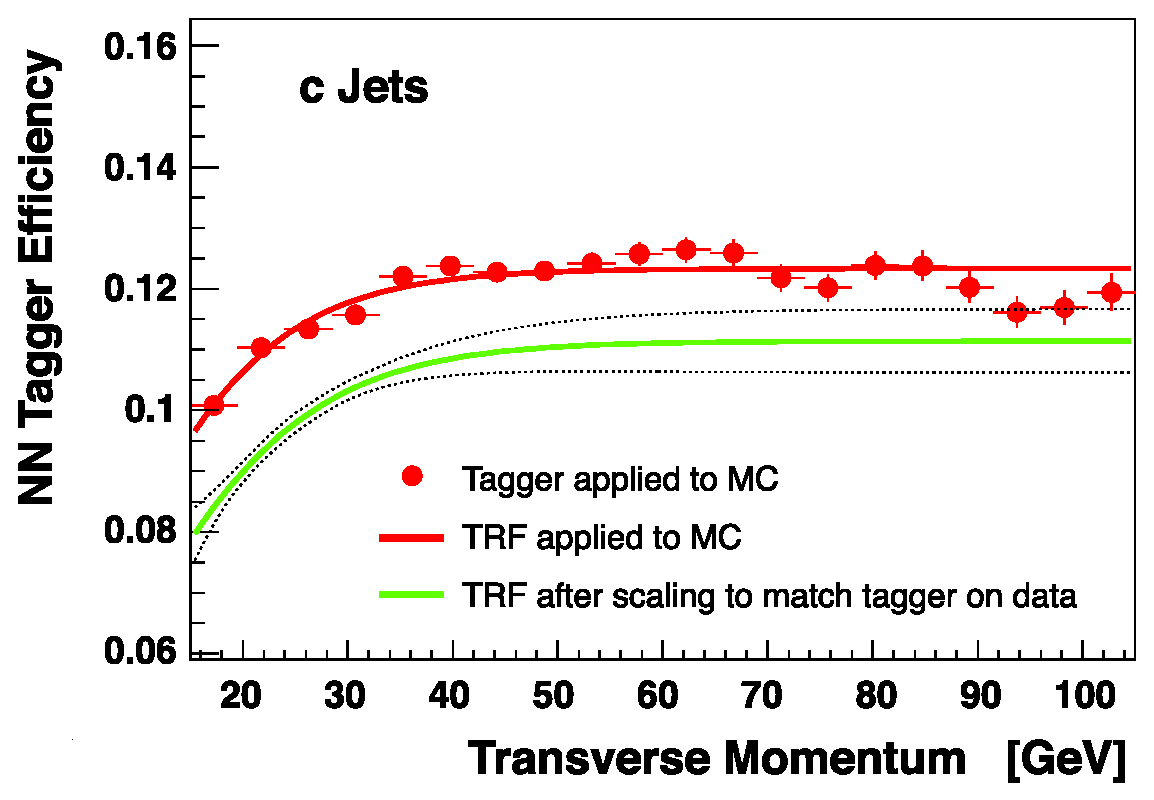
\includegraphics[width=0.32\textwidth]
{figures/TRF_c_pt.eps}
\hspace{0.6in}
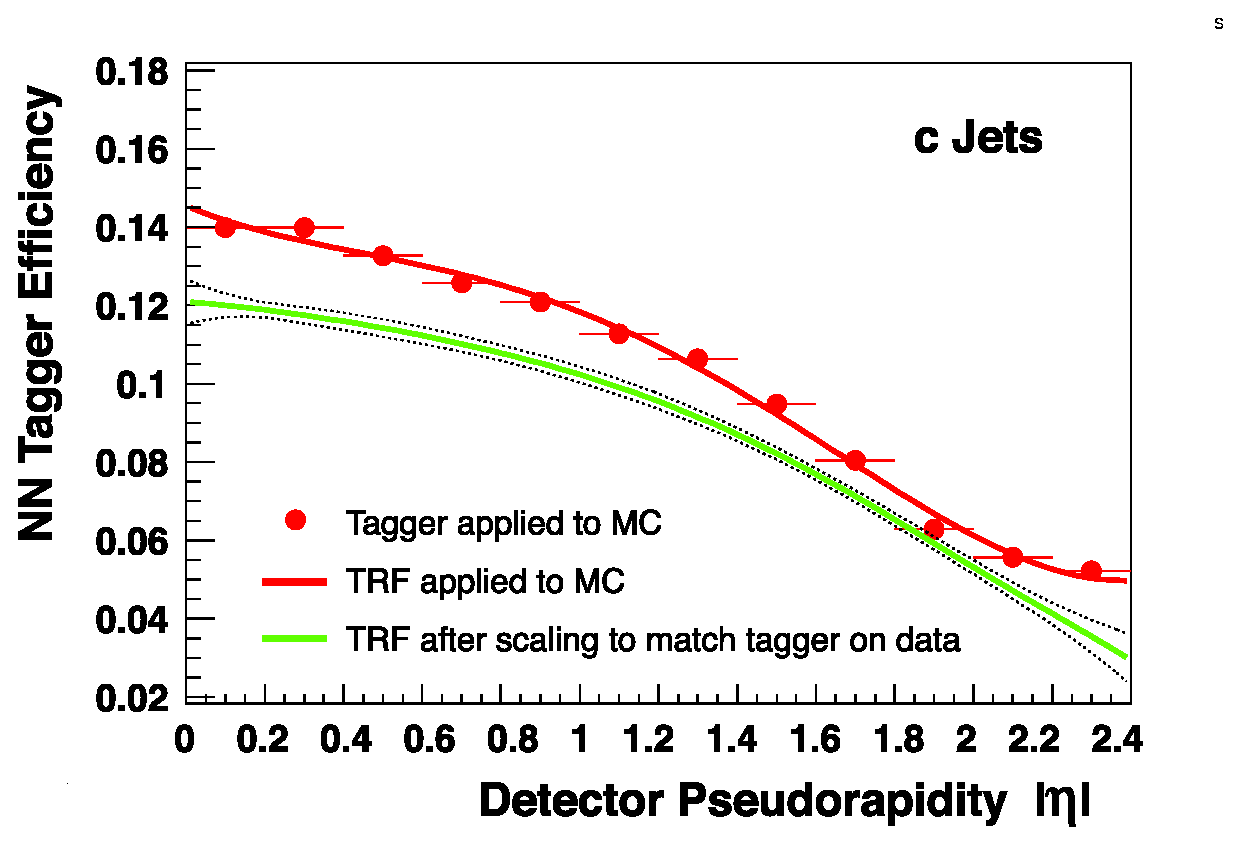
\includegraphics[width=0.35\textwidth]
{figures/TRF_c_eta.eps}
\vspace{-0.1in}
\begin{minipage}{5.5in}
\caption[nntagrf]{NN TIGHT tagger $b$-jet (upper row) and $c$-jet
(lower row) efficiencies as a function of $\pt$ (left column) and
$\eta$ (right column) in the inclusive $b$ and $c$ MC samples. The
corresponding data tag-rate functions ($\varepsilon_b$ and
$\varepsilon_c$) are also displayed.}
\label{fig:NNTRFs}
\end{minipage}
\end{figure}

\clearpage

The negative tag rate ($\varepsilon^{-}_{\rm data}$) measured in EM
and QCD data skims is used to estimate the fake, or mistag rate
$\varepsilon_{light}$. Each of the three taggers used as inputs for
the NN define a \emph{negative tag} differently: CSIP and JLIP as a
secondary vertex with negative impact parameter significance with
respect to the primary vertex, and SVT as a vertex with negative decay
length and $\Delta R<0.5$ with the jet. The NN tagger defines a
negative tag as the ouput from the NN when all three other taggers
yield a negative tag.

\vspace{0.1in}
The fake-tag rate $\varepsilon_{\rm light}$ is derived from the
negative tag rate, but needs to be corrected for the residual presence
of $b$- and $c$-quark jets in the negative tags and the asymmetry
between positive and negative tags. Two scale factors derived in MC
account for this:
\begin{eqnarray*}
\varepsilon_{\rm light}
& = & \varepsilon^{-}_{\rm data} \times SF_{hf} \times SF_{ll} \\
SF_{hf}
& = & \varepsilon^{-}_{\rm QCD~light}/\varepsilon^{-}_{\rm QCD~all} \\
SF_{ll}
& = & \varepsilon^{+}_{\rm QCD~light}/\varepsilon^{-}_{\rm QCD~light},
\end{eqnarray*}
where $SF_{hf}$ is the ratio between the number of negative tagged
jets from light quarks over the total number of negative tagged jets
in the QCD Monte Carlo. It is smaller than one if heavy-flavor jets
are present. And $SF_{ll}$ is the ratio between the number of positive
tagged jets from light quarks over the number of negative tagged jets
from light quarks in the QCD Monte Carlo. It is sensitive to
long-lived hadron decays in light-quark jets.


\subsection{$b$-Tagging Event Weights and $b$-Jet Assignment
Combinations}
\label{permuter}

Given the three different efficiencies $\varepsilon_{\alpha}$ outlined
above for $\alpha$ = $b$, $c$ and light jets, the probability to tag a
jet of flavor $\alpha$, or Tag Rate Function (TRF) can be expressed as
the product of the taggability and the tagging efficiency:
$$
\mathcal{P}_{\alpha}(\pt,\eta) = P^{\rm taggable}(\pt,\eta)\times \varepsilon_{\alpha}(\pt,\eta)
$$
Using the per jet probability, we can deduce the event probability
to contain zero, one or more than two tags:
\begin{eqnarray*}
P_{\rm event}(0~{\rm tag}) & = & \prod_{j=1}^{\rm N_{jets}}(1 - \mathcal{P}_{\alpha_j}(\pt_j,\eta_j)) \\
P_{\rm event}(1~{\rm tag}) & = & \sum_{j=1}^{\rm
N_{jets}}\mathcal{P}_{\alpha_j}(\pt_j,\eta_j) \prod_{i\neq j}(1 - \mathcal{P}_{\alpha_i}(\pt_i,\eta_i)) \\
P_{\rm event}(2~{\rm tags}) & = &
\sum_{j=1}^{\rm N_{jets}}\mathcal{P}_{\alpha_j}(\pt_j,\eta_j)
\prod_{i\neq j}\mathcal{P}_{\alpha_i}(\pt_i,\eta_i)
\prod_{k\neq j \neq i}(1 - \mathcal{P}_{\alpha_k}(\pt_k,\eta_k))
\end{eqnarray*}

By using TRFs we can estimate the number of tagged events, but this
does not help in knowing whether an individual jet is tagged or not,
since the TRF returns a weight. If one wants to use kinematic
variables using tagged or untagged jets, one needs to split each event
based on the number of jets and the number of possible tags and assign
for each permutation which jet or jets are tagged/untagged, with the
corresponding weight. Therefore each event is taken into account
several times, making sure that the sum of weights for all possible
combinations in each event returns the original probability for the
event to be not-tagged, tagged once or tagged twice.  This method
allows to use kinematic variables that rely on using $b$-tagging
information on the jets.
 

%---------------------------------------------------------------------
%---------------------------------------------------------------------
%% Plots after selection                    # 5
\clearpage
\input{appendix_selectionplots}

%---------------------------------------------------------------------
%---------------------------------------------------------------------
% Many tables of systematic uncertainties   # 6
\clearpage
%---------------------------------------------------------------------
%  Writeup of the fall 2006 search of Run II data for single top quark
%  production at DZero.
%  Started Oct 2006
%  Authors: The Single Top Working Group
%---------------------------------------------------------------------
%
\appendix
\section*{Appendix 6 --- Systematic Uncertainty Tables}
\label{appendix-systematics}


Tables~\ref{sys-error-CC-EqOneTag-EqOneJet}--\ref{sys-error-mu-EqTwoTag-EqFourJet}
show the flat systematic uncertainties on the signal and background
samples for the single-tagged and two double-tagged analyses. We also
have two systematics sources that affect the shapes of the
distributions, the jet energy scale uncertainty and the tag-rate
functions uncertainty. These effects are not included in the tables.

Here are some brief explanations of the terms listed in the
tables. The tables can be used to see the correlation between the
various samples and analysis channels for each uncertainty. A
systematic uncertainty is assumed to be fully correlated between all
signal or background samples within a given row in each table, and for
rows with the same name in different tables. The exceptions to this
are the systematic uncertainties on the theoretical cross sections
used to normalize the MC backgrounds (except for the two {\ttbar}
backgrounds), and the statistical uncertainty from the size of each MC
sample.

Note that owing to the normalization to data before $b$~tagging, the
$Wb\bar{b}$, $Wc\bar{c}$, and $Wjj$ tagged yield estimates are not
affected by any of the systematic uncertainties that affect the
overall yield. The exception to this is $b$~tagging, which is applied
after normalization. There is still an effect on the shapes of
distributions from the uncertainty components that depend on event
kinematics. For these shape-changing systematics (jet energy scale and
tag-rate functions), we include the uncertainty in each bin of the
binned likelihood fit.

The row ``Matrix Method'' in each table includes not only the matrix
method uncertainties but also the flavor composition uncertainty in
the $W$+jets samples, which is by far the dominant component.  The
normalization for $Wb\bar{b}$, $Wc\bar{c}$, and $Wjj$ includes the
other MC backgrounds and thus their uncertainties in principle also
affect $Wbb$, $Wcc$, and $Wjj$.  However, the other MC backgrounds
only contribute about 3\% to the pretagged yield, which means their
uncertainties are negligible compared with the other matrix method
uncertainties and thus we ignore them.

As a further result of the normalization before $b$~tagging, the
uncertainties for the different $W$+jets samples are anti-correlated
with the uncertainties for the fake-lepton sample. We take this into
account in the calculation by computing an overal uncertainty on the
sum of $W$+jets and fake-lepton. They are listed separately in the row
``Matrix Method'', but in the calculation, the uncertainty is
evaluated on the sum of the yields.

Tables~\ref{sys-error-CC-EqOneTag-EqOneJet}--\ref{sys-error-mu-EqTwoTag-EqFourJet}
show the total uncertainty on each background component separately,
with the statistical and systematic parts combined in quadrature in
the final lines. Note, the uncertainties for the zero-tagged channels
are the same as for the single-tagged ones, so are not shown
separately. The luminosity, cross section and branching fraction for
the $tb$ and $tqb$ signals are not used for the signal acceptance
during the cross section calculation but only when yields are quoted.
They are presented in parentheses in the following tables.

\clearpage

\begin{center}
UNCERTAINTIES FOR SINGLE-TAGGED ELECTRON ANALYSES
\end{center}

\begin{table}[!h!tbp]
\begin{center}
\begin{minipage}{5 in}
\begin{ruledtabular}
\begin{tabular}{lcccccccc}
 & \multicolumn{8}{c}
{\underline{Single-Tagged One-Jet Electron Channel Percentage
Errors}}\\
 & $tb$  & $tqb$ & ${\ttbar}lj$ & ${\ttbar}ll$ & $Wbb$ & $Wcc$
 & $Wjj$ & Mis-ID $e$ \\
\hline
\multicolumn{4}{l}
{\underline{Components for Normalization}}  &  &  &  &    \\
%%%%%%%%%%%%%%%%%%%%%%% Insert content of syslatex file here
%
%##########################################################
%#
%# systematic uncertainties table
%## for tagger Electron_EqOneTag_EqOneJet
%# 
%# file create on Wed Nov 15 09:14:27 2006
%#
%#
%# all errors are given as relative errors in percent.
%#
%#
%                               tb   tqb    ttlj    ttll  Wbb    Wcc    Wjj      QCD
~~Luminosity            &  (   6.1)          &  (   6.1)
                        &     6.1    &     6.1
                        &  ---                                 &  ---
                        &  ---				       &  ---					\\
~~Cross section         &  (  16.0)         &  (  15.0)
                        &    18.0   &    18.0
                        &  ---                                 &  ---
                        &  ---                                 &  ---					\\
~~Branching fraction    &  (   1.0)          &  (   1.0)
                        &     1.0    &     1.0
                        &  ---                                 &  ---
                        &  ---                                 &  ---					\\
~~Matrix method         &  ---				       &  ---
			&  ---				       &  ---
                        &    16.8                  &    16.8
                        &    16.8                  &    16.8			\\
~~Primary vertex        &     2.4         &     2.4
                        &     2.4 &     2.4
                        &  ---                                 &  ---
                        &  ---                                 &  ---					\\
~~Electron ID           &     5.5                  &     5.5
                        &     5.5          &     5.5
                        &  ---                                 &  ---
                        &  ---                                 &  ---					\\
~~Jet ID                &     1.5                  &     1.5
                        &     1.5          &     1.5
                        &  ---                                 &  ---
                        &  ---                                 &  ---					\\
~~Jet fragmentation     &     5.0               &     5.0
                        &     7.0       &     5.0
                        &  ---                                 &  ---
                        &  ---                                 &  ---					\\
~~Trigger               &     3.0               &     3.0
                        &     3.0       &     3.0
                        &  ---                                 &  ---
                        &  ---                                 &  ---					\\
\multicolumn{4}{l}
{\underline{Components for Normalization and Shape}}           &  &  &  &				\\
~~Jet energy scale      &     1.4                   &     0.3
                        &     9.9           &     1.7
                        &  ---                                 &  ---
                        &  ---                                 &  ---					\\
~~Flavor-dependent TRFs &     6.4                   &     6.2
                        &     6.8           &     6.5
                        &     5.9                  &     6.6
                        &     7.2                  &  ---					\\
\underline{Statistics}  &     0.8                       &     0.8
                        &     1.3               &     0.6
                        &     0.9                      &     0.9
                        &     0.4		       &     6.4			\\
\underline{Combined}                                           &  &  &  &  &  &  &		\\
~~Acceptance uncertainty
                        &    12.4                 &    12.2
			&  ---				       &  ---
			&  ---				       &  ---
                        &  ---                                 &  ---					\\
~~Yield uncertainty
                        &    20.2                  &    19.4
                        &    24.6          &    21.9
                        &    17.9                 &    18.1
                        &    18.3		       &    18.0			\\
�

%
%%%%%%%%%%%%%%%%%%%%%%%
\end{tabular}
\end{ruledtabular}
\vspace{-0.15in}
\caption{Electron channel uncertainties, requiring exactly one tag
and one jet.}
\label{sys-error-CC-EqOneTag-EqOneJet}
\end{minipage}
\end{center}
\end{table}

\begin{table}[!h!tbp]
\begin{center}
\begin{minipage}{5 in}
\begin{ruledtabular}
\begin{tabular}{lcccccccc}
 & \multicolumn{8}{c}
{\underline{Single-Tagged Two-Jets Electron Channel Percentage
Errors}}\\
 & $tb$  & $tqb$ & ${\ttbar}lj$ & ${\ttbar}ll$ & $Wbb$ & $Wcc$
 & $Wjj$ & Mis-ID $e$ \\
\hline
\multicolumn{4}{l}
{\underline{Components for Normalization}}  &  &  &  &    \\
%%%%%%%%%%%%%%%%%%%%%%% Insert content of syslatex file here
%
%##########################################################
%#
%# systematic uncertainties table
%## for tagger Electron_EqOneTag_EqTwoJet
%# 
%# file create on Wed Nov 15 09:14:27 2006
%#
%#
%# all errors are given as relative errors in percent.
%#
%#
%                               tb   tqb    ttlj    ttll  Wbb    Wcc    Wjj      QCD
~~Luminosity            &  (   6.1)          &  (   6.1)
                        &     6.1    &     6.1
                        &  ---                                 &  ---
                        &  ---				       &  ---					\\
~~Cross section         &  (  16.0)         &  (  15.0)
                        &    18.0   &    18.0
                        &  ---                                 &  ---
                        &  ---                                 &  ---					\\
~~Branching fraction    &  (   1.0)          &  (   1.0)
                        &     1.0    &     1.0
                        &  ---                                 &  ---
                        &  ---                                 &  ---					\\
~~Matrix method         &  ---				       &  ---
			&  ---				       &  ---
                        &    18.2                  &    18.2
                        &    18.2                  &    18.2			\\
~~Primary vertex        &     2.4         &     2.4
                        &     2.4 &     2.4
                        &  ---                                 &  ---
                        &  ---                                 &  ---					\\
~~Electron ID           &     5.5                  &     5.5
                        &     5.5          &     5.5
                        &  ---                                 &  ---
                        &  ---                                 &  ---					\\
~~Jet ID                &     1.5                  &     1.5
                        &     1.5          &     1.5
                        &  ---                                 &  ---
                        &  ---                                 &  ---					\\
~~Jet fragmentation     &     5.0               &     5.0
                        &     7.0       &     5.0
                        &  ---                                 &  ---
                        &  ---                                 &  ---					\\
~~Trigger               &     3.0               &     3.0
                        &     3.0       &     3.0
                        &  ---                                 &  ---
                        &  ---                                 &  ---					\\
\multicolumn{4}{l}
{\underline{Components for Normalization and Shape}}           &  &  &  &				\\
~~Jet energy scale      &     1.4                   &     0.3
                        &     9.9           &     1.7
                        &  ---                                 &  ---
                        &  ---                                 &  ---					\\
~~Flavor-dependent TRFs &     2.1                   &     5.9
                        &     4.6           &     2.4
                        &     4.4                  &     6.3
                        &     7.4                  &  ---					\\
\underline{Statistics}  &     0.7                       &     0.7
                        &     1.3               &     0.8
                        &     0.9                      &     0.9
                        &     0.4		       &     5.6			\\
\underline{Combined}                                           &  &  &  &  &  &  &		\\
~~Acceptance uncertainty
                        &    10.8                 &    12.1
			&  ---				       &  ---
			&  ---				       &  ---
                        &  ---                                 &  ---					\\
~~Yield uncertainty
                        &    19.3                  &    19.3
                        &    24.1          &    21.1
                        &    18.8                 &    19.3
                        &    19.7		       &    19.1			\\
�

%
%%%%%%%%%%%%%%%%%%%%%%%
\end{tabular}
\end{ruledtabular}
\vspace{-0.15in}
\caption{Electron channel uncertainties, requiring exactly one tag
and two jets.}
\label{sys-error-CC-EqOneTag-EqTwoJet}
\end{minipage}
\end{center}
\end{table}

\clearpage

\begin{center}
UNCERTAINTIES FOR SINGLE-TAGGED ELECTRON ANALYSES
\end{center}

\begin{table}[!h!tbp]
\begin{center}
\begin{minipage}{5 in}
\begin{ruledtabular}
\begin{tabular}{lcccccccc}
 & \multicolumn{8}{c}
{\underline{Single-Tagged Three-Jets Electron Channel Percentage
Errors}}\\
 & $tb$  & $tqb$ & ${\ttbar}lj$ & ${\ttbar}ll$ & $Wbb$ & $Wcc$
 & $Wjj$ & Mis-ID $e$ \\
\hline
\multicolumn{4}{l}
{\underline{Components for Normalization}}  &  &  &  &    \\
%%%%%%%%%%%%%%%%%%%%%%% Insert content of syslatex file here
%
%##########################################################
%#
%# systematic uncertainties table
%## for tagger Electron_EqOneTag_EqThreeJet
%# 
%# file create on Wed Nov 15 09:14:27 2006
%#
%#
%# all errors are given as relative errors in percent.
%#
%#
%                               tb   tqb    ttlj    ttll  Wbb    Wcc    Wjj      QCD
~~Luminosity            &  (   6.1)          &  (   6.1)
                        &     6.1    &     6.1
                        &  ---                                 &  ---
                        &  ---				       &  ---					\\
~~Cross section         &  (  16.0)         &  (  15.0)
                        &    18.0   &    18.0
                        &  ---                                 &  ---
                        &  ---                                 &  ---					\\
~~Branching fraction    &  (   1.0)          &  (   1.0)
                        &     1.0    &     1.0
                        &  ---                                 &  ---
                        &  ---                                 &  ---					\\
~~Matrix method         &  ---				       &  ---
			&  ---				       &  ---
                        &    16.8                  &    16.8
                        &    16.8                  &    16.8			\\
~~Primary vertex        &     2.4         &     2.4
                        &     2.4 &     2.4
                        &  ---                                 &  ---
                        &  ---                                 &  ---					\\
~~Electron ID           &     5.5                  &     5.5
                        &     5.5          &     5.5
                        &  ---                                 &  ---
                        &  ---                                 &  ---					\\
~~Jet ID                &     1.5                  &     1.5
                        &     1.5          &     1.5
                        &  ---                                 &  ---
                        &  ---                                 &  ---					\\
~~Jet fragmentation     &     5.0               &     5.0
                        &     7.0       &     5.0
                        &  ---                                 &  ---
                        &  ---                                 &  ---					\\
~~Trigger               &     3.0               &     3.0
                        &     3.0       &     3.0
                        &  ---                                 &  ---
                        &  ---                                 &  ---					\\
\multicolumn{4}{l}
{\underline{Components for Normalization and Shape}}           &  &  &  &				\\
~~Jet energy scale      &     5.3                   &     5.8
                        &     4.1           &     3.2
                        &  ---                                 &  ---
                        &  ---                                 &  ---					\\
~~Flavor-dependent TRFs &     2.1                   &     4.5
                        &     2.9           &     2.1
                        &     4.4                  &     6.2
                        &     7.6                  &  ---					\\
\underline{Statistics}  &     1.0                       &     1.0
                        &     0.5               &     0.5
                        &     1.0                      &     1.0
                        &     0.5		       &     6.7			\\
\underline{Combined}                                           &  &  &  &  &  &  &		\\
~~Acceptance uncertainty
                        &    12.0                 &    12.9
			&  ---				       &  ---
			&  ---				       &  ---
                        &  ---                                 &  ---					\\
~~Yield uncertainty
                        &    20.0                  &    19.8
                        &    22.0          &    21.2
                        &    17.4                 &    18.0
                        &    18.5		       &    18.1			\\
�

%
%%%%%%%%%%%%%%%%%%%%%%%
\end{tabular}
\end{ruledtabular}
\vspace{-0.15in}
\caption{Electron channel uncertainties, requiring exactly one tag
and three jets.}
\label{sys-error-CC-EqOneTag-EqThreeJet}
\end{minipage}
\end{center}
\end{table}

\begin{table}[!h!tbp]
\begin{center}
\begin{minipage}{5 in}
\begin{ruledtabular}
\begin{tabular}{lcccccccc}
 & \multicolumn{8}{c}
{\underline{Single-Tagged Four-Jets Electron Channel Percentage
Errors}}\\
 & $tb$  & $tqb$ & ${\ttbar}lj$ & ${\ttbar}ll$ & $Wbb$ & $Wcc$
 & $Wjj$ & Mis-ID $e$ \\
\hline
\multicolumn{4}{l}
{\underline{Components for Normalization}}  &  &  &  &    \\
%%%%%%%%%%%%%%%%%%%%%%% Insert content of syslatex file here
%
%##########################################################
%#
%# systematic uncertainties table
%## for tagger Electron_EqOneTag_EqFourJet
%# 
%# file create on Wed Nov 15 09:14:28 2006
%#
%#
%# all errors are given as relative errors in percent.
%#
%#
%                               tb   tqb    ttlj    ttll  Wbb    Wcc    Wjj      QCD
~~Luminosity            &  (   6.1)          &  (   6.1)
                        &     6.1    &     6.1
                        &  ---                                 &  ---
                        &  ---				       &  ---					\\
~~Cross section         &  (  16.0)         &  (  15.0)
                        &    18.0   &    18.0
                        &  ---                                 &  ---
                        &  ---                                 &  ---					\\
~~Branching fraction    &  (   1.0)          &  (   1.0)
                        &     1.0    &     1.0
                        &  ---                                 &  ---
                        &  ---                                 &  ---					\\
~~Matrix method         &  ---				       &  ---
			&  ---				       &  ---
                        &    17.6                  &    17.6
                        &    17.6                  &    17.6			\\
~~Primary vertex        &     2.4         &     2.4
                        &     2.4 &     2.4
                        &  ---                                 &  ---
                        &  ---                                 &  ---					\\
~~Electron ID           &     5.5                  &     5.5
                        &     5.5          &     5.5
                        &  ---                                 &  ---
                        &  ---                                 &  ---					\\
~~Jet ID                &     1.5                  &     1.5
                        &     1.5          &     1.5
                        &  ---                                 &  ---
                        &  ---                                 &  ---					\\
~~Jet fragmentation     &     5.0               &     5.0
                        &     7.0       &     5.0
                        &  ---                                 &  ---
                        &  ---                                 &  ---					\\
~~Trigger               &     3.0               &     3.0
                        &     3.0       &     3.0
                        &  ---                                 &  ---
                        &  ---                                 &  ---					\\
\multicolumn{4}{l}
{\underline{Components for Normalization and Shape}}           &  &  &  &				\\
~~Jet energy scale      &    11.8                   &    10.4
                        &     1.4           &     7.6
                        &  ---                                 &  ---
                        &  ---                                 &  ---					\\
~~Flavor-dependent TRFs &     2.1                   &     3.6
                        &     1.9           &     2.1
                        &     4.5                  &     6.2
                        &     7.7                  &  ---					\\
\underline{Statistics}  &     2.0                       &     2.0
                        &     0.7               &     1.0
                        &     2.0                      &     1.0
                        &     0.8		       &    10.2			\\
\underline{Combined}                                           &  &  &  &  &  &  &		\\
~~Acceptance uncertainty
                        &    16.1                 &    15.3
			&  ---				       &  ---
			&  ---				       &  ---
                        &  ---                                 &  ---					\\
~~Yield uncertainty
                        &    22.7                  &    21.5
                        &    21.6          &    22.3
                        &    18.3                 &    18.7
                        &    19.3		       &    20.3			\\
�

%
%%%%%%%%%%%%%%%%%%%%%%%
\end{tabular}
\end{ruledtabular}
\vspace{-0.15in}
\caption{Electron channel uncertainties, requiring exactly one tag
and four jets.}
\label{sys-error-CC-EqOneTag-EqFourJet}
\end{minipage}
\end{center}
\end{table}

\clearpage

\begin{center}
UNCERTAINTIES FOR SINGLE-TAGGED MUON ANALYSES
\end{center}

\begin{table}[!h!tbp]
\begin{center}
\begin{minipage}{5 in}
\begin{ruledtabular}
\begin{tabular}{lcccccccc}
 & \multicolumn{8}{c}
{\underline{Single-Tagged One-Jet Muon Channel Percentage Errors}}\\
 & $tb$  & $tqb$ & ${\ttbar}lj$ & ${\ttbar}ll$ & $Wbb$ & $Wcc$
 & $Wjj$ & Mis-ID $e$ \\
\hline
\multicolumn{4}{l}
{\underline{Components for Normalization}}  &  &  &  &    \\
%%%%%%%%%%%%%%%%%%%%%%% Insert content of syslatex file here
%
%##########################################################
%#
%# systematic uncertainties table
%## for tagger Muon_EqOneTag_EqOneJet
%# 
%# file create on Wed Nov 15 09:14:26 2006
%#
%#
%# all errors are given as relative errors in percent.
%#
%#
%                               tb   tqb    ttlj    ttll  Wbb    Wcc    Wjj      QCD
~~Luminosity            &  (   6.1)          &  (   6.1)
                        &     6.1    &     6.1
                        &  ---                                 &  ---
                        &  ---				       &  ---					\\
~~Cross section         &  (  16.0)         &  (  15.0)
                        &    18.0   &    18.0
                        &  ---                                 &  ---
                        &  ---                                 &  ---					\\
~~Branching fraction    &  (   1.0)          &  (   1.0)
                        &     1.0    &     1.0
                        &  ---                                 &  ---
                        &  ---                                 &  ---					\\
~~Matrix method         &  ---				       &  ---
			&  ---				       &  ---
                        &    17.4                  &    17.4
                        &    17.4                  &    17.4			\\
~~Primary vertex        &     3.0         &     3.0
                        &     3.0 &     3.0
                        &  ---                                 &  ---
                        &  ---                                 &  ---					\\
~~Muon ID           &     7.4                  &     7.4
                        &     7.4          &     7.4
                        &  ---                                 &  ---
                        &  ---                                 &  ---					\\
~~Jet ID                &     1.5                  &     1.5
                        &     1.5          &     1.5
                        &  ---                                 &  ---
                        &  ---                                 &  ---					\\
~~Jet fragmentation     &     5.0               &     5.0
                        &     7.0       &     5.0
                        &  ---                                 &  ---
                        &  ---                                 &  ---					\\
~~Trigger               &     6.0               &     6.0
                        &     6.0       &     6.0
                        &  ---                                 &  ---
                        &  ---                                 &  ---					\\
\multicolumn{4}{l}
{\underline{Components for Normalization and Shape}}           &  &  &  &				\\
~~Jet energy scale      &     5.3                   &     6.1
                        &    20.1           &     6.8
                        &  ---                                 &  ---
                        &  ---                                 &  ---					\\
~~Flavor-dependent TRFs &     6.4                   &     6.2
                        &     6.7           &     6.5
                        &     6.1                  &     6.8
                        &     7.4                  &  ---					\\
\underline{Statistics}  &     9.0                       &     0.7
                        &     1.0               &     0.7
                        &     0.8                      &     0.7
                        &     0.4		       &    18.0			\\
\underline{Combined}                                           &  &  &  &  &  &  &		\\
~~Acceptance uncertainty
                        &    17.7                 &    15.5
			&  ---				       &  ---
			&  ---				       &  ---
                        &  ---                                 &  ---					\\
~~Yield uncertainty
                        &    23.9                  &    21.6
                        &    31.1          &    24.0
                        &    18.5                 &    18.7
                        &    19.0		       &    25.0			\\
�

%
%%%%%%%%%%%%%%%%%%%%%%%
\end{tabular}
\end{ruledtabular}
\vspace{-0.15in}
\caption{Muon channel uncertainties, requiring exactly one tag and
one jet.}
\label{sys-error-mu-EqOneTag-EqOneJet}
\end{minipage}
\end{center}
\end{table}

\begin{table}[!h!tbp]
\begin{center}
\begin{minipage}{5 in}
\begin{ruledtabular}
\begin{tabular}{lcccccccc}
 & \multicolumn{8}{c}
{\underline{Single-Tagged Two-Jets Muon Channel Percentage Errors}}\\
 & $tb$  & $tqb$ & ${\ttbar}lj$ & ${\ttbar}ll$ & $Wbb$ & $Wcc$
 & $Wjj$ & Mis-ID $e$ \\
\hline
\multicolumn{4}{l}
{\underline{Components for Normalization}}  &  &  &  &    \\
%%%%%%%%%%%%%%%%%%%%%%% Insert content of syslatex file here
%
%##########################################################
%#
%# systematic uncertainties table
%## for tagger Muon_EqOneTag_EqTwoJet
%# 
%# file create on Wed Nov 15 09:14:26 2006
%#
%#
%# all errors are given as relative errors in percent.
%#
%#
%                               tb   tqb    ttlj    ttll  Wbb    Wcc    Wjj      QCD
~~Luminosity            &  (   6.1)          &  (   6.1)
                        &     6.1    &     6.1
                        &  ---                                 &  ---
                        &  ---				       &  ---					\\
~~Cross section         &  (  16.0)         &  (  15.0)
                        &    18.0   &    18.0
                        &  ---                                 &  ---
                        &  ---                                 &  ---					\\
~~Branching fraction    &  (   1.0)          &  (   1.0)
                        &     1.0    &     1.0
                        &  ---                                 &  ---
                        &  ---                                 &  ---					\\
~~Matrix method         &  ---				       &  ---
			&  ---				       &  ---
                        &    20.7                  &    20.7
                        &    20.7                  &    20.7			\\
~~Primary vertex        &     3.0         &     3.0
                        &     3.0 &     3.0
                        &  ---                                 &  ---
                        &  ---                                 &  ---					\\
~~Muon ID           &     7.4                  &     7.4
                        &     7.4          &     7.4
                        &  ---                                 &  ---
                        &  ---                                 &  ---					\\
~~Jet ID                &     1.5                  &     1.5
                        &     1.5          &     1.5
                        &  ---                                 &  ---
                        &  ---                                 &  ---					\\
~~Jet fragmentation     &     5.0               &     5.0
                        &     7.0       &     5.0
                        &  ---                                 &  ---
                        &  ---                                 &  ---					\\
~~Trigger               &     6.0               &     6.0
                        &     6.0       &     6.0
                        &  ---                                 &  ---
                        &  ---                                 &  ---					\\
\multicolumn{4}{l}
{\underline{Components for Normalization and Shape}}           &  &  &  &				\\
~~Jet energy scale      &     5.3                   &     6.1
                        &    20.1           &     6.8
                        &  ---                                 &  ---
                        &  ---                                 &  ---					\\
~~Flavor-dependent TRFs &     1.8                   &     5.9
                        &     4.5           &     2.0
                        &     4.4                  &     6.3
                        &     7.5                  &  ---					\\
\underline{Statistics}  &     9.0                       &     0.7
                        &     1.0               &     1.0
                        &     0.8                      &     0.8
                        &     0.4		       &    14.0			\\
\underline{Combined}                                           &  &  &  &  &  &  &		\\
~~Acceptance uncertainty
                        &    16.7                 &    15.4
			&  ---				       &  ---
			&  ---				       &  ---
                        &  ---                                 &  ---					\\
~~Yield uncertainty
                        &    23.1                  &    21.5
                        &    30.7          &    23.2
                        &    21.2                 &    21.7
                        &    22.0		       &    25.0			\\
�

%
%%%%%%%%%%%%%%%%%%%%%%%
\end{tabular}
\end{ruledtabular}
\vspace{-0.15in}
\caption{Muon channel uncertainties, requiring exactly one tag and
two jets.}
\label{sys-error-mu-EqOneTag-EqTwoJet}
\end{minipage}
\end{center}
\end{table}

\clearpage

\begin{center}
UNCERTAINTIES FOR SINGLE-TAGGED MUON ANALYSES
\end{center}

\begin{table}[!h!tbp]
\begin{center}
\begin{minipage}{5 in}
\begin{ruledtabular}
\begin{tabular}{lcccccccc}
 & \multicolumn{8}{c}
{\underline{Single-Tagged Three-Jets Muon Channel Percentage
Errors}}\\
 & $tb$  & $tqb$ & ${\ttbar}lj$ & ${\ttbar}ll$ & $Wbb$ & $Wcc$
 & $Wjj$ & Mis-ID $e$ \\
\hline
\multicolumn{4}{l}
{\underline{Components for Normalization}}  &  &  &  &    \\
%%%%%%%%%%%%%%%%%%%%%%% Insert content of syslatex file here
%
%##########################################################
%#
%# systematic uncertainties table
%## for tagger Muon_EqOneTag_EqThreeJet
%# 
%# file create on Wed Nov 15 09:14:26 2006
%#
%#
%# all errors are given as relative errors in percent.
%#
%#
%                               tb   tqb    ttlj    ttll  Wbb    Wcc    Wjj      QCD
~~Luminosity            &  (   6.1)          &  (   6.1)
                        &     6.1    &     6.1
                        &  ---                                 &  ---
                        &  ---				       &  ---					\\
~~Cross section         &  (  16.0)         &  (  15.0)
                        &    18.0   &    18.0
                        &  ---                                 &  ---
                        &  ---                                 &  ---					\\
~~Branching fraction    &  (   1.0)          &  (   1.0)
                        &     1.0    &     1.0
                        &  ---                                 &  ---
                        &  ---                                 &  ---					\\
~~Matrix method         &  ---				       &  ---
			&  ---				       &  ---
                        &    20.8                  &    20.8
                        &    20.8                  &    20.8			\\
~~Primary vertex        &     3.0         &     3.0
                        &     3.0 &     3.0
                        &  ---                                 &  ---
                        &  ---                                 &  ---					\\
~~Muon ID           &     7.4                  &     7.4
                        &     7.4          &     7.4
                        &  ---                                 &  ---
                        &  ---                                 &  ---					\\
~~Jet ID                &     1.5                  &     1.5
                        &     1.5          &     1.5
                        &  ---                                 &  ---
                        &  ---                                 &  ---					\\
~~Jet fragmentation     &     5.0               &     5.0
                        &     7.0       &     5.0
                        &  ---                                 &  ---
                        &  ---                                 &  ---					\\
~~Trigger               &     6.0               &     6.0
                        &     6.0       &     6.0
                        &  ---                                 &  ---
                        &  ---                                 &  ---					\\
\multicolumn{4}{l}
{\underline{Components for Normalization and Shape}}           &  &  &  &				\\
~~Jet energy scale      &     9.3                   &     9.0
                        &    10.8           &     7.6
                        &  ---                                 &  ---
                        &  ---                                 &  ---					\\
~~Flavor-dependent TRFs &     1.8                   &     4.4
                        &     2.6           &     1.9
                        &     4.3                  &     6.2
                        &     7.6                  &  ---					\\
\underline{Statistics}  &     2.0                       &     2.0
                        &     0.8               &     0.7
                        &     1.0                      &     1.0
                        &     0.7		       &    14.3			\\
\underline{Combined}                                           &  &  &  &  &  &  &		\\
~~Acceptance uncertainty
                        &    16.1                 &    16.5
			&  ---				       &  ---
			&  ---				       &  ---
                        &  ---                                 &  ---					\\
~~Yield uncertainty
                        &    22.7                  &    22.3
                        &    25.2          &    23.5
                        &    21.2                 &    21.7
                        &    22.1		       &    25.2			\\
�

%
%%%%%%%%%%%%%%%%%%%%%%%
\end{tabular}
\end{ruledtabular}
\vspace{-0.15in}
\caption{Muon channel uncertainties, requiring exactly one tag and
three jets.}
\label{sys-error-mu-EqOneTag-EqThreeJet}
\end{minipage}
\end{center}
\end{table}

\begin{table}[!h!tbp]
\begin{center}
\begin{minipage}{5 in}
\begin{ruledtabular}
\begin{tabular}{lcccccccc}
 & \multicolumn{8}{c}
{\underline{Single-Tagged Four-Jets Muon Channel Percentage Errors}}\\
 & $tb$  & $tqb$ & ${\ttbar}lj$ & ${\ttbar}ll$ & $Wbb$ & $Wcc$
 & $Wjj$ & Mis-ID $e$ \\
\hline
\multicolumn{4}{l}
{\underline{Components for Normalization}}  &  &  &  &    \\
%%%%%%%%%%%%%%%%%%%%%%% Insert content of syslatex file here
%
%##########################################################
%#
%# systematic uncertainties table
%## for tagger Muon_EqOneTag_EqFourJet
%# 
%# file create on Wed Nov 15 09:14:27 2006
%#
%#
%# all errors are given as relative errors in percent.
%#
%#
%                               tb   tqb    ttlj    ttll  Wbb    Wcc    Wjj      QCD
~~Luminosity            &  (   6.1)          &  (   6.1)
                        &     6.1    &     6.1
                        &  ---                                 &  ---
                        &  ---				       &  ---					\\
~~Cross section         &  (  16.0)         &  (  15.0)
                        &    18.0   &    18.0
                        &  ---                                 &  ---
                        &  ---                                 &  ---					\\
~~Branching fraction    &  (   1.0)          &  (   1.0)
                        &     1.0    &     1.0
                        &  ---                                 &  ---
                        &  ---                                 &  ---					\\
~~Matrix method         &  ---				       &  ---
			&  ---				       &  ---
                        &    20.6                  &    20.6
                        &    20.6                  &    20.6			\\
~~Primary vertex        &     3.0         &     3.0
                        &     3.0 &     3.0
                        &  ---                                 &  ---
                        &  ---                                 &  ---					\\
~~Muon ID           &     7.4                  &     7.4
                        &     7.4          &     7.4
                        &  ---                                 &  ---
                        &  ---                                 &  ---					\\
~~Jet ID                &     1.5                  &     1.5
                        &     1.5          &     1.5
                        &  ---                                 &  ---
                        &  ---                                 &  ---					\\
~~Jet fragmentation     &     5.0               &     5.0
                        &     7.0       &     5.0
                        &  ---                                 &  ---
                        &  ---                                 &  ---					\\
~~Trigger               &     6.0               &     6.0
                        &     6.0       &     6.0
                        &  ---                                 &  ---
                        &  ---                                 &  ---					\\
\multicolumn{4}{l}
{\underline{Components for Normalization and Shape}}           &  &  &  &				\\
~~Jet energy scale      &    14.6                   &    14.6
                        &     7.1           &    10.9
                        &  ---                                 &  ---
                        &  ---                                 &  ---					\\
~~Flavor-dependent TRFs &     1.9                   &     3.4
                        &     1.6           &     1.8
                        &     4.3                  &     6.1
                        &     7.7                  &  ---					\\
\underline{Statistics}  &     2.0                       &     2.0
                        &     0.7               &     1.0
                        &     2.0                      &     2.0
                        &     1.0		       &    21.8			\\
\underline{Combined}                                           &  &  &  &  &  &  &		\\
~~Acceptance uncertainty
                        &    19.6                 &    19.9
			&  ---				       &  ---
			&  ---				       &  ---
                        &  ---                                 &  ---					\\
~~Yield uncertainty
                        &    25.3                  &    24.9
                        &    23.8          &    24.7
                        &    21.1                 &    21.6
                        &    22.0		       &    30.0			\\
�

%
%%%%%%%%%%%%%%%%%%%%%%%
\end{tabular}
\end{ruledtabular}
\vspace{-0.15in}
\caption{Muon channel uncertainties, requiring exactly one tag and
four jets.}
\label{sys-error-mu-EqOneTag-EqFourJet}
\end{minipage}
\end{center}
\end{table}

\clearpage

\begin{center}
UNCERTAINTIES FOR DOUBLE-TAGGED ELECTRON ANALYSES
\end{center}

\begin{table}[!h!tbp]
\begin{center}
\begin{minipage}{5 in}
\begin{ruledtabular}
\begin{tabular}{lcccccccc}
 & \multicolumn{8}{c}
{\underline{Double-Tagged Two-Jets Electron Channel Percentage
Errors}}\\
 & $tb$  & $tqb$ & ${\ttbar}lj$ & ${\ttbar}ll$ & $Wbb$ & $Wcc$
 & $Wjj$ & Mis-ID $e$ \\
\hline
\multicolumn{4}{l}
{\underline{Components for Normalization}}  &  &  &  &    \\
%%%%%%%%%%%%%%%%%%%%%%% Insert content of syslatex file here
%
%##########################################################
%#
%# systematic uncertainties table
%## for tagger Electron_EqTwoTag_EqTwoJet
%# 
%# file create on Wed Nov 15 09:14:28 2006
%#
%#
%# all errors are given as relative errors in percent.
%#
%#
%                               tb   tqb    ttlj    ttll  Wbb    Wcc    Wjj      QCD
~~Luminosity            &  (   6.1)          &  (   6.1)
                        &     6.1    &     6.1
                        &  ---                                 &  ---
                        &  ---				       &  ---					\\
~~Cross section         &  (  16.0)         &  (  15.0)
                        &    18.0   &    18.0
                        &  ---                                 &  ---
                        &  ---                                 &  ---					\\
~~Branching fraction    &  (   1.0)          &  (   1.0)
                        &     1.0    &     1.0
                        &  ---                                 &  ---
                        &  ---                                 &  ---					\\
~~Matrix method         &  ---				       &  ---
			&  ---				       &  ---
                        &    26.5                  &    26.5
                        &    26.5                  &    26.5			\\
~~Primary vertex        &     2.4         &     2.4
                        &     2.4 &     2.4
                        &  ---                                 &  ---
                        &  ---                                 &  ---					\\
~~Electron ID           &     5.5                  &     5.5
                        &     5.5          &     5.5
                        &  ---                                 &  ---
                        &  ---                                 &  ---					\\
~~Jet ID                &     1.5                  &     1.5
                        &     1.5          &     1.5
                        &  ---                                 &  ---
                        &  ---                                 &  ---					\\
~~Jet fragmentation     &     5.0               &     5.0
                        &     7.0       &     5.0
                        &  ---                                 &  ---
                        &  ---                                 &  ---					\\
~~Trigger               &     3.0               &     3.0
                        &     3.0       &     3.0
                        &  ---                                 &  ---
                        &  ---                                 &  ---					\\
\multicolumn{4}{l}
{\underline{Components for Normalization and Shape}}           &  &  &  &				\\
~~Jet energy scale      &     0.8                   &     4.1
                        &     8.0           &     1.8
                        &  ---                                 &  ---
                        &  ---                                 &  ---					\\
~~Flavor-dependent TRFs &    12.9                   &    12.9
                        &    13.5           &    13.0
                        &    12.2                  &    13.6
                        &    16.1                  &  ---					\\
\underline{Statistics}  &     0.7                       &     0.7
                        &     1.3               &     0.8
                        &     0.9                      &     0.9
                        &     0.4		       &    28.9			\\
\underline{Combined}                                           &  &  &  &  &  &  &		\\
~~Acceptance uncertainty
                        &    16.7                 &    17.2
			&  ---				       &  ---
			&  ---				       &  ---
                        &  ---                                 &  ---					\\
~~Yield uncertainty
                        &    23.1                  &    22.8
                        &    26.6          &    24.6
                        &    29.1                 &    29.8
                        &    31.0		       &    39.2			\\
�

%
%%%%%%%%%%%%%%%%%%%%%%%
\end{tabular}
\end{ruledtabular}
\vspace{-0.15in}
\caption{Electron channel uncertainties, requiring exactly two tags
and two jets.}
\label{sys-error-CC-EqTwoTag-EqTwoJet}
\end{minipage}
\end{center}
\end{table}

\begin{table}[!h!tbp]
\begin{center}
\begin{minipage}{5 in}
\begin{ruledtabular}
\begin{tabular}{lcccccccc}
 & \multicolumn{8}{c}
{\underline{Double-Tagged Three-Jets Electron Channel Percentage
Errors}}\\
 & $tb$  & $tqb$ & ${\ttbar}lj$ & ${\ttbar}ll$ & $Wbb$ & $Wcc$
 & $Wjj$ & Mis-ID $e$ \\
\hline
\multicolumn{4}{l}
{\underline{Components for Normalization}}  &  &  &  &    \\
%%%%%%%%%%%%%%%%%%%%%%% Insert content of syslatex file here
%
%##########################################################
%#
%# systematic uncertainties table
%## for tagger Electron_EqTwoTag_EqThreeJet
%# 
%# file create on Wed Nov 15 09:14:28 2006
%#
%#
%# all errors are given as relative errors in percent.
%#
%#
%                               tb   tqb    ttlj    ttll  Wbb    Wcc    Wjj      QCD
~~Luminosity            &  (   6.1)          &  (   6.1)
                        &     6.1    &     6.1
                        &  ---                                 &  ---
                        &  ---				       &  ---					\\
~~Cross section         &  (  16.0)         &  (  15.0)
                        &    18.0   &    18.0
                        &  ---                                 &  ---
                        &  ---                                 &  ---					\\
~~Branching fraction    &  (   1.0)          &  (   1.0)
                        &     1.0    &     1.0
                        &  ---                                 &  ---
                        &  ---                                 &  ---					\\
~~Matrix method         &  ---				       &  ---
			&  ---				       &  ---
                        &    22.1                  &    22.1
                        &    22.1                  &    22.1			\\
~~Primary vertex        &     2.4         &     2.4
                        &     2.4 &     2.4
                        &  ---                                 &  ---
                        &  ---                                 &  ---					\\
~~Electron ID           &     5.5                  &     5.5
                        &     5.5          &     5.5
                        &  ---                                 &  ---
                        &  ---                                 &  ---					\\
~~Jet ID                &     1.5                  &     1.5
                        &     1.5          &     1.5
                        &  ---                                 &  ---
                        &  ---                                 &  ---					\\
~~Jet fragmentation     &     5.0               &     5.0
                        &     7.0       &     5.0
                        &  ---                                 &  ---
                        &  ---                                 &  ---					\\
~~Trigger               &     3.0               &     3.0
                        &     3.0       &     3.0
                        &  ---                                 &  ---
                        &  ---                                 &  ---					\\
\multicolumn{4}{l}
{\underline{Components for Normalization and Shape}}           &  &  &  &				\\
~~Jet energy scale      &     4.8                   &     4.0
                        &     3.5           &     2.9
                        &  ---                                 &  ---
                        &  ---                                 &  ---					\\
~~Flavor-dependent TRFs &    12.7                   &    12.4
                        &    12.6           &    12.8
                        &    12.0                  &    13.3
                        &    16.4                  &  ---					\\
\underline{Statistics}  &     1.0                       &     1.0
                        &     0.7               &     0.7
                        &     1.0                      &     1.0
                        &     0.5		       &    25.8			\\
\underline{Combined}                                           &  &  &  &  &  &  &		\\
~~Acceptance uncertainty
                        &    17.2                 &    16.8
			&  ---				       &  ---
			&  ---				       &  ---
                        &  ---                                 &  ---					\\
~~Yield uncertainty
                        &    23.5                  &    22.5
                        &    25.1          &    24.6
                        &    25.2                 &    25.8
                        &    27.5		       &    34.0			\\
�

%
%%%%%%%%%%%%%%%%%%%%%%%
\end{tabular}
\end{ruledtabular}
\vspace{-0.15in}
\caption{Electron channel uncertainties, requiring exactly two tags
and three jets.}
\label{sys-error-CC-EqTwoTag-EqThreeJet}
\end{minipage}
\end{center}
\end{table}

\clearpage

\begin{center}
UNCERTAINTIES FOR DOUBLE-TAGGED ELECTRON ANALYSES
\end{center}

\begin{table}[!h!tbp]
\begin{center}
\begin{minipage}{5 in}
\begin{ruledtabular}
\begin{tabular}{lcccccccc}
 & \multicolumn{8}{c}
{\underline{Double-Tagged Four-Jets Electron Channel Percentage
Errors}}\\
 & $tb$  & $tqb$ & ${\ttbar}lj$ & ${\ttbar}ll$ & $Wbb$ & $Wcc$
 & $Wjj$ & Mis-ID $e$ \\
\hline
\multicolumn{4}{l}
{\underline{Components for Normalization}}  &  &  &  &    \\
%%%%%%%%%%%%%%%%%%%%%%% Insert content of syslatex file here
%
%##########################################################
%#
%# systematic uncertainties table
%## for tagger Electron_EqTwoTag_EqFourJet
%# 
%# file create on Wed Nov 15 09:14:28 2006
%#
%#
%# all errors are given as relative errors in percent.
%#
%#
%                               tb   tqb    ttlj    ttll  Wbb    Wcc    Wjj      QCD
~~Luminosity            &  (   6.1)          &  (   6.1)
                        &     6.1    &     6.1
                        &  ---                                 &  ---
                        &  ---				       &  ---					\\
~~Cross section         &  (  16.0)         &  (  15.0)
                        &    18.0   &    18.0
                        &  ---                                 &  ---
                        &  ---                                 &  ---					\\
~~Branching fraction    &  (   1.0)          &  (   1.0)
                        &     1.0    &     1.0
                        &  ---                                 &  ---
                        &  ---                                 &  ---					\\
~~Matrix method         &  ---				       &  ---
			&  ---				       &  ---
                        &    19.5                  &    19.5
                        &    19.5                  &    19.5			\\
~~Primary vertex        &     2.4         &     2.4
                        &     2.4 &     2.4
                        &  ---                                 &  ---
                        &  ---                                 &  ---					\\
~~Electron ID           &     5.5                  &     5.5
                        &     5.5          &     5.5
                        &  ---                                 &  ---
                        &  ---                                 &  ---					\\
~~Jet ID                &     1.5                  &     1.5
                        &     1.5          &     1.5
                        &  ---                                 &  ---
                        &  ---                                 &  ---					\\
~~Jet fragmentation     &     5.0               &     5.0
                        &     7.0       &     5.0
                        &  ---                                 &  ---
                        &  ---                                 &  ---					\\
~~Trigger               &     3.0               &     3.0
                        &     3.0       &     3.0
                        &  ---                                 &  ---
                        &  ---                                 &  ---					\\
\multicolumn{4}{l}
{\underline{Components for Normalization and Shape}}           &  &  &  &				\\
~~Jet energy scale      &    10.9                   &     8.3
                        &     1.6           &     7.6
                        &  ---                                 &  ---
                        &  ---                                 &  ---					\\
~~Flavor-dependent TRFs &    12.5                   &    12.2
                        &    12.0           &    12.6
                        &    12.0                  &    13.2
                        &    16.6                  &  ---					\\
\underline{Statistics}  &     2.0                       &     2.0
                        &     0.7               &     1.0
                        &     2.0                      &     1.0
                        &     0.8		       &    26.7			\\
\underline{Combined}                                           &  &  &  &  &  &  &		\\
~~Acceptance uncertainty
                        &    19.8                 &    18.2
			&  ---				       &  ---
			&  ---				       &  ---
                        &  ---                                 &  ---					\\
~~Yield uncertainty
                        &    25.4                  &    23.6
                        &    24.6          &    25.5
                        &    23.0                 &    23.6
                        &    25.6		       &    33.1			\\
�

%
%%%%%%%%%%%%%%%%%%%%%%%
\end{tabular}
\end{ruledtabular}
\vspace{-0.15in}
\caption{Electron channel uncertainties, requiring exactly two tags
and four jets.}
\label{sys-error-CC-EqTwoTag-EqFourJet}
\end{minipage}
\end{center}
\end{table}

\clearpage

\begin{center}
UNCERTAINTIES FOR DOUBLE-TAGGED MUON ANALYSES
\end{center}

\begin{table}[!h!tbp]
\begin{center}
\begin{minipage}{5 in}
\begin{ruledtabular}
\begin{tabular}{lcccccccc}
 & \multicolumn{8}{c}
{\underline{Double-Tagged Two-Jets Muon Channel Percentage Errors}}\\
 & $tb$  & $tqb$ & ${\ttbar}lj$ & ${\ttbar}ll$ & $Wbb$ & $Wcc$
 & $Wjj$ & Mis-ID $e$ \\
\hline
\multicolumn{4}{l}
{\underline{Components for Normalization}}  &  &  &  &    \\
%%%%%%%%%%%%%%%%%%%%%%% Insert content of syslatex file here
%
%##########################################################
%#
%# systematic uncertainties table
%## for tagger Muon_EqTwoTag_EqTwoJet
%# 
%# file create on Wed Nov 15 09:14:27 2006
%#
%#
%# all errors are given as relative errors in percent.
%#
%#
%                               tb   tqb    ttlj    ttll  Wbb    Wcc    Wjj      QCD
~~Luminosity            &  (   6.1)          &  (   6.1)
                        &     6.1    &     6.1
                        &  ---                                 &  ---
                        &  ---				       &  ---					\\
~~Cross section         &  (  16.0)         &  (  15.0)
                        &    18.0   &    18.0
                        &  ---                                 &  ---
                        &  ---                                 &  ---					\\
~~Branching fraction    &  (   1.0)          &  (   1.0)
                        &     1.0    &     1.0
                        &  ---                                 &  ---
                        &  ---                                 &  ---					\\
~~Matrix method         &  ---				       &  ---
			&  ---				       &  ---
                        &    27.6                  &    27.6
                        &    27.6                  &    27.6			\\
~~Primary vertex        &     3.0         &     3.0
                        &     3.0 &     3.0
                        &  ---                                 &  ---
                        &  ---                                 &  ---					\\
~~Muon ID           &     7.4                  &     7.4
                        &     7.4          &     7.4
                        &  ---                                 &  ---
                        &  ---                                 &  ---					\\
~~Jet ID                &     1.5                  &     1.5
                        &     1.5          &     1.5
                        &  ---                                 &  ---
                        &  ---                                 &  ---					\\
~~Jet fragmentation     &     5.0               &     5.0
                        &     7.0       &     5.0
                        &  ---                                 &  ---
                        &  ---                                 &  ---					\\
~~Trigger               &     6.0               &     6.0
                        &     6.0       &     6.0
                        &  ---                                 &  ---
                        &  ---                                 &  ---					\\
\multicolumn{4}{l}
{\underline{Components for Normalization and Shape}}           &  &  &  &				\\
~~Jet energy scale      &     5.2                   &     9.1
                        &    19.7           &     6.9
                        &  ---                                 &  ---
                        &  ---                                 &  ---					\\
~~Flavor-dependent TRFs &    12.9                   &    12.8
                        &    13.4           &    12.9
                        &    12.2                  &    13.5
                        &    16.1                  &  ---					\\
\underline{Statistics}  &     1.3                       &     0.9
                        &     0.7               &     0.7
                        &     1.0                      &     1.0
                        &     0.5		       &    57.7			\\
\underline{Combined}                                           &  &  &  &  &  &  &		\\
~~Acceptance uncertainty
                        &    19.0                 &    20.3
			&  ---				       &  ---
			&  ---				       &  ---
                        &  ---                                 &  ---					\\
~~Yield uncertainty
                        &    24.8                  &    25.2
                        &    32.9          &    26.5
                        &    30.2                 &    30.7
                        &    31.9		       &    64.0			\\
�

%
%%%%%%%%%%%%%%%%%%%%%%%
\end{tabular}
\end{ruledtabular}
\vspace{-0.15in}
\caption{Muon channel uncertainties, requiring exactly two tags and
two jets.}
\label{sys-error-mu-EqTwoTag-EqTwoJet}
\end{minipage}
\end{center}
\end{table}

\begin{table}[!h!tbp]
\begin{center}
\begin{minipage}{5 in}
\begin{ruledtabular}
\begin{tabular}{lcccccccc}
 & \multicolumn{8}{c}
{\underline{Double-Tagged Three-Jets Muon Channel Percentage
Errors}}\\
 & $tb$  & $tqb$ & ${\ttbar}lj$ & ${\ttbar}ll$ & $Wbb$ & $Wcc$
 & $Wjj$ & Mis-ID $e$ \\
\hline
\multicolumn{4}{l}
{\underline{Components for Normalization}}  &  &  &  &    \\
%%%%%%%%%%%%%%%%%%%%%%% Insert content of syslatex file here
%
%##########################################################
%#
%# systematic uncertainties table
%## for tagger Muon_EqTwoTag_EqThreeJet
%# 
%# file create on Wed Nov 15 09:14:27 2006
%#
%#
%# all errors are given as relative errors in percent.
%#
%#
%                               tb   tqb    ttlj    ttll  Wbb    Wcc    Wjj      QCD
~~Luminosity            &  (   6.1)          &  (   6.1)
                        &     6.1    &     6.1
                        &  ---                                 &  ---
                        &  ---				       &  ---					\\
~~Cross section         &  (  16.0)         &  (  15.0)
                        &    18.0   &    18.0
                        &  ---                                 &  ---
                        &  ---                                 &  ---					\\
~~Branching fraction    &  (   1.0)          &  (   1.0)
                        &     1.0    &     1.0
                        &  ---                                 &  ---
                        &  ---                                 &  ---					\\
~~Matrix method         &  ---				       &  ---
			&  ---				       &  ---
                        &    25.0                  &    25.0
                        &    25.0                  &    25.0			\\
~~Primary vertex        &     3.0         &     3.0
                        &     3.0 &     3.0
                        &  ---                                 &  ---
                        &  ---                                 &  ---					\\
~~Muon ID           &     7.4                  &     7.4
                        &     7.4          &     7.4
                        &  ---                                 &  ---
                        &  ---                                 &  ---					\\
~~Jet ID                &     1.5                  &     1.5
                        &     1.5          &     1.5
                        &  ---                                 &  ---
                        &  ---                                 &  ---					\\
~~Jet fragmentation     &     5.0               &     5.0
                        &     7.0       &     5.0
                        &  ---                                 &  ---
                        &  ---                                 &  ---					\\
~~Trigger               &     6.0               &     6.0
                        &     6.0       &     6.0
                        &  ---                                 &  ---
                        &  ---                                 &  ---					\\
\multicolumn{4}{l}
{\underline{Components for Normalization and Shape}}           &  &  &  &				\\
~~Jet energy scale      &    10.2                   &     7.6
                        &    10.1           &     7.8
                        &  ---                                 &  ---
                        &  ---                                 &  ---					\\
~~Flavor-dependent TRFs &    12.6                   &    12.3
                        &    12.4           &    12.7
                        &    12.0                  &    13.1
                        &    16.4                  &  ---					\\
\underline{Statistics}  &     2.0                       &     2.0
                        &     0.8               &     0.6
                        &     1.0                      &     1.0
                        &     0.6		       &    50.0			\\
\underline{Combined}                                           &  &  &  &  &  &  &		\\
~~Acceptance uncertainty
                        &    20.8                 &    19.4
			&  ---				       &  ---
			&  ---				       &  ---
                        &  ---                                 &  ---					\\
~~Yield uncertainty
                        &    26.3                  &    24.5
                        &    27.7          &    26.7
                        &    27.7                 &    28.2
                        &    29.9		       &    55.9			\\
�

%
%%%%%%%%%%%%%%%%%%%%%%%
\end{tabular}
\end{ruledtabular}
\vspace{-0.15in}
\caption{Muon channel uncertainties, requiring exactly two tags and
three jets.}
\label{sys-error-mu-EqTwoTag-EqThreeJet}
\end{minipage}
\end{center}
\end{table}

\clearpage

\begin{center}
UNCERTAINTIES FOR DOUBLE-TAGGED MUON ANALYSES
\end{center}

\begin{table}[!h!tbp]
\begin{center}
\begin{minipage}{5 in}
\begin{ruledtabular}
\begin{tabular}{lcccccccc}
 & \multicolumn{8}{c}
{\underline{Double-Tagged Four-Jets Muon Channel Percentage Errors}}\\
 & $tb$  & $tqb$ & ${\ttbar}lj$ & ${\ttbar}ll$ & $Wbb$ & $Wcc$
 & $Wjj$ & Mis-ID $e$ \\
\hline
\multicolumn{4}{l}
{\underline{Components for Normalization}}  &  &  &  &    \\
%%%%%%%%%%%%%%%%%%%%%%% Insert content of syslatex file here
%
%##########################################################
%#
%# systematic uncertainties table
%## for tagger Muon_EqTwoTag_EqFourJet
%# 
%# file create on Wed Nov 15 09:14:27 2006
%#
%#
%# all errors are given as relative errors in percent.
%#
%#
%                               tb   tqb    ttlj    ttll  Wbb    Wcc    Wjj      QCD
~~Luminosity            &  (   6.1)          &  (   6.1)
                        &     6.1    &     6.1
                        &  ---                                 &  ---
                        &  ---				       &  ---					\\
~~Cross section         &  (  16.0)         &  (  15.0)
                        &    18.0   &    18.0
                        &  ---                                 &  ---
                        &  ---                                 &  ---					\\
~~Branching fraction    &  (   1.0)          &  (   1.0)
                        &     1.0    &     1.0
                        &  ---                                 &  ---
                        &  ---                                 &  ---					\\
~~Matrix method         &  ---				       &  ---
			&  ---				       &  ---
                        &    26.5                  &    26.5
                        &    26.5                  &    26.5			\\
~~Primary vertex        &     3.0         &     3.0
                        &     3.0 &     3.0
                        &  ---                                 &  ---
                        &  ---                                 &  ---					\\
~~Muon ID           &     7.4                  &     7.4
                        &     7.4          &     7.4
                        &  ---                                 &  ---
                        &  ---                                 &  ---					\\
~~Jet ID                &     1.5                  &     1.5
                        &     1.5          &     1.5
                        &  ---                                 &  ---
                        &  ---                                 &  ---					\\
~~Jet fragmentation     &     5.0               &     5.0
                        &     7.0       &     5.0
                        &  ---                                 &  ---
                        &  ---                                 &  ---					\\
~~Trigger               &     6.0               &     6.0
                        &     6.0       &     6.0
                        &  ---                                 &  ---
                        &  ---                                 &  ---					\\
\multicolumn{4}{l}
{\underline{Components for Normalization and Shape}}           &  &  &  &				\\
~~Jet energy scale      &     1.6                   &    15.0
                        &     7.0           &    11.5
                        &  ---                                 &  ---
                        &  ---                                 &  ---					\\
~~Flavor-dependent TRFs &    12.4                   &    12.1
                        &    11.8           &    12.4
                        &    11.7                  &    13.3
                        &    16.5                  &  ---					\\
\underline{Statistics}  &     2.0                       &     2.0
                        &     0.7               &     1.0
                        &     2.0                      &     2.0
                        &     1.0		       &   100.0			\\
\underline{Combined}                                           &  &  &  &  &  &  &		\\
~~Acceptance uncertainty
                        &    18.0                 &    23.2
			&  ---				       &  ---
			&  ---				       &  ---
                        &  ---                                 &  ---					\\
~~Yield uncertainty
                        &    24.1                  &    27.6
                        &    26.5          &    27.9
                        &    29.0                 &    29.7
                        &    31.2		       &   103.4			\\
�

%
%%%%%%%%%%%%%%%%%%%%%%%
\end{tabular}
\end{ruledtabular}
\vspace{-0.15in}
\caption{Muon channel uncertainties, requiring exactly two tags and
four jets.}
\label{sys-error-mu-EqTwoTag-EqFourJet}
\end{minipage}
\end{center}
\end{table}




%---------------------------------------------------------------------
%---------------------------------------------------------------------
%% Cross check samples                      # 7
\clearpage
\input{appendix_crosschecks}

%---------------------------------------------------------------------
%---------------------------------------------------------------------
%% Cross check samples                      # 8
\clearpage
\input{appendix_ensembles}

%---------------------------------------------------------------------
%---------------------------------------------------------------------
%% How we optimized the discriminants       # 9
\clearpage
%---------------------------------------------------------------------
%

\appendix
\section*{Appendix 9 --- Discriminant Optimization Criteria}
\label{appendix-optimization}

Since the goal of the analysis is to validate the production of single
top quarks, any optimization criteria should be based on affirming the
signal+background hypothesis convincingly. We, therefore, define an
optimal search as one that maximizes the probability of the
signal+background hypothesis relative to that of the background
hypothesis. Since we use a Bayesian approach for all our statistical
analyses, a natural way to do this would be to compute the Bayes
factor which is the ratio of the posterior probability densities of
the signal+background hypothesis to the background-only
hypothesis. The description of the method we use to obtain a posterior
probability density can be found in Appendix 13 of
Ref.~\cite{run2-d0-230} and in Ref.~\cite{d0note5123}.

A fundamental principle of Bayesian reasoning is that one should
integrate over all that is unknown.  In designing an analysis, we do
not yet know the event count $n$, nor do we know the background and
signal means $b$ and $s$, respectively. Therefore, in accordance with
the basic Bayesian principle, we must integrate over $n$, $s$, and $b$,
constrained by whatever knowledge we have of them.

We are working to develop the methodology to compute Bayes factor as
discussed above by averaging over all possible value of $n$, $s$ and
$b$~\cite{d0note5260}. For now we have used an approximation to the
Bayes factor by considering only one value of $n$ which is set to the
estimated values of the signal and background yields. The factor is
then computed as illustrated in Fig.~\ref{fig:bayesfactor} using the
values of the posterior probability densities at peak and at zero
signal cross section.

\begin{figure}[!h!tbp]
\includegraphics[width=0.5\textwidth]{figures/bayesfactor.eps}
\vspace{-0.1in}
\begin{minipage}{4in}
\caption[bayesfactor]{A plot of the posterior probability density
versus signal cross section that illustrates the calculation of the
Bayes factor.}
\label{fig:bayesfactor}
\end{minipage}
\end{figure}

We have chosen to use the Bayes ratio to optimize the discriminants'
performance. It may be noted however that this approximate definition
may yield unreasonably high values as the posterior density at zero
signal cross section becomes infinitesimally small. In such a case the
distribution of the posterior probability density is expected to be a
near-perfect Gaussian, and a more meaningful quantity for any
optimization would be a ratio of the signal cross section at the peak
of the posterior to the width of the posterior as shown in
Fig.~\ref{fig:measurement}. This essentially defines how significant a
measurement of the single top cross section would be if the data were
consistent with the signal+background hypothesis.

\begin{figure}[!h!tbp]
\includegraphics[width=0.5\textwidth]{figures/measurement.eps}
\vspace{-0.1in}
\begin{minipage}{4in}
\caption[measurement]{A plot of the posterior probability density
versus signal cross section that illustrates the measurement of the
cross section and its uncertainty.}
\label{fig:measurement}
\end{minipage}
\end{figure}




%---------------------------------------------------------------------
%---------------------------------------------------------------------
%% How we measure the signal significance   # 10
\clearpage
%---------------------------------------------------------------------
%  Writeup of the improved search of Run II data for single top quark
%  production at DZero.
%  Started: Oct 2006
%  Authors: The Single Top Working Group
%---------------------------------------------------------------------
%

\appendix
\section*{Appendix 10 --- Measure of Significance}
\label{appendix-significance}

The term ``significance'' has different definitions depending on our
goal. If the goal is to define the single top signal significance,
then an appropriate definition would be the ratio of the signal cross
section at the peak of the posterior probability density to the width
of the posterior, as defined in Appendix~9, which is inversely
proportional to the uncertainty on the cross section measurement.

However, if the goal is to define the significance of excess in data
over background, then one possible definition is the
p-value~\cite{Fisher}. For Poisson data, the p-value is the
probability to get a count equal to or greater than the count
observed, assuming that the count is due to background only. The
background hypothesis, in this context, is the {\em null hypothesis},
that is, the hypothesis we seek to reject. Fisher, who invented it,
saw the p-value as a measure of evidence against the null. If the
p-value is sufficiently small one may well consider rejecting the null
in favor of the hypothesis that something other than background is
present. Therefore a significantly small p-value would indicate how
``significant'' enough the excess of events over background is, to
claim a discovery.

%The p-value is a well-defined statistical quantity in the so-called
%frequentist approach. However, it can be computed only if the null
%hypothesis (in this case, the background) can be stated precisely. In
%order to take into account the uncertainties in our background
%estimation, one defines a hybrid approach by doing a Bayesian
%integration over the background prior. Details of the implementation
%of the p-value with background uncertainties, and using spectral
%distributions can be found in~\cite{d0note5258}.

%There are many ways to define ``a'' p-value. 
%\begin{itemize}
%\item In a purely frequentist approach, we can generate fake
%data-sets with no signal and re-run the whole analysis obtaining a
%result for each one of these ``ensembles''. The number of ensembles
%that yield a result equal to the observed or higher, divided by the
%total number of ensembles is the p-value. 
%\item A hybrid method that starts from the background estimate and
%takes the uncertainties in to account by integrating over the
%background prior, as described in ~\cite{d0note5258}.
%\item Another commonly used method in the field is the modifed
%frequentist approach.
%\end{itemize}

We can generate multiple pseudo-datasets containing only background
events and run them through the analysis exactly as if they were the
real data events, and obtain a cross section from each one of
them. The p-value can then be calculated as the number of these
ensembles that yield a result equal to the observed or higher, divided
by the total number of ensembles.

To generate these ensembles, we use background events from our model
and treat the fluctuations of each background source separately. We
draw random events from each background source separately, as
indicated by the allowed variation due to systematic and statistical
uncertainties. The event weights are taken into account such that
events with a higher weight will be more likely to be picked. The
variance of the background events is large: we start from 1.34M
electron events and 1.28M muon events, then only consider the two
thirds of these that have not been used in the discriminant
training. The nominal background yields are 755 electron events and
643 muon events. Thus, each ensemble is generated picking around 700
events from around 850,000. The source of background most affected by
oversampling is multijets, since some channels contain very few events
that will be picked repeatedly. Given that the multijet background is
very small and the statistical errors dominate, this does not
introduce a large bias.

The ensemble generation includes a flat (i.e., normalization only, not
shape changing) 20\% error for the {\ttbar} yield ($N_{\ttbar}$),
which represents approximately the overall yield uncertainty from all
systematic effects combined (see Appendix~6). The shift in the
{\ttbar} yield:
$$
N_{\ttbar}^{\prime}
= N_{\ttbar}\times {\rm Gaussian}({\rm mean=1},{\rm width=0.2})
$$
is the same for electrons and muons. The treatment of the $W$+jets and
multijet backgrounds accounts for the normalization to data from the
matrix method and for the effect of $b$-tagging. The error from the
matrix method normalization of $W$+jets and multijet events is
incorporated in the ensemble generation by letting each sample
(multijets, $Wc\bar{c}$, $Wb\bar{b}$ and $Wjj$) fluctuate with a
different random number $r$ sampled from a Gaussian distribution:
\begin{eqnarray*}
r_{\rm QCD} = {\rm Gaussian}(1,0.2) \\
r_{Wjj}     = {\rm Gaussian}(1,0.2) \\
r_{Wbb}     = {\rm Gaussian}(1,0.2) \\
r_{Wcc}     = {\rm Gaussian}(1,0.2) 
\end{eqnarray*}

The background sum of $W$+jets and multijets yields $N_{\rm WQCD}$ is
fluctuated to become $N_{\rm WQCD}^{\prime}$:
\begin{eqnarray*}
N_{\rm WQCD}          &=& N_{\rm QCD} + N_{Wjj} + N_{Wbb} + N_{Wcc} \\
N_{\rm WQCD}^{\prime} &=& r_{\rm QCD}\times N_{\rm QCD}
                        + r_{Wjj}    \times N_{Wjj}
                        + r_{Wbb}    \times N_{Wbb}
                        + r_{Wcc}    \times N_{Wcc}
\end{eqnarray*}
These two expressions fix the normalization to data. What is changed
here is the composition of each of the subcomponents. Once the
correlation between multijets and $W$+jets is taken care of, we also
need to take into account the effect of $b$-tagging. We split the
summed samples of $W$+jets and multijets into 1-tag and 2-tags
sets. The average uncertainty on these samples is 5\% and 12\%
respectively (see Appendix~6), so we form a scale factor $S^{\rm
tag}_{\rm WQCD}$ that incorporates the different rates for tagging
single- and double-tagged events in these samples:
\begin{eqnarray*}
r_{\rm 1tag} &=& {\rm Gaussian}(1,0.05) \\
r_{\rm 2tag} &=& {\rm Gaussian}(1,0.12) \\
S^{\rm tag}_{\rm WQCD}
             &=& \frac{r_{\rm 1tag} \times N^{\rm 1tag}_{\rm WQCD}
                    +  r_{\rm 2tag} \times N^{\rm 2tag}_{\rm WQCD}}
                {N^{\rm 1tag}_{\rm WQCD} + N^{\rm 2tag}_{\rm WQCD}}
\end{eqnarray*}

Finally, the multijets and $W$+jets event yields are fluctuated to:
$$
N_{i}^{\prime} = r_{i} \times \frac{N_{\rm WQCD}}
                                   {N_{\rm WQCD}^{\prime}}
                       \times S_{\rm tag}^{\rm WQCD}
                       \times N_{i} ~;~ i = {\rm QCD}, Wjj, Wbb, Wcc
$$

Once each background source has been fluctuated, we randomly pick
events based on a Poisson distribution of the new systematics-shifted
total background sum:
$$
N_{\rm Data}^{\prime} = N_{\rm QCD}^{\prime}
                      + N_{Wjj}^{\prime}
                      + N_{Wbb}^{\prime}
                      + N_{Wcc}^{\prime}
                      + N_{\ttbar}^{\prime}
$$

We have generated about 60,000 ensembles of pseudo-data with this
method that we use to measure the signifince or p-value of our search.


%---------------------------------------------------------------------
}
%---------------------------------------------------------------------
%---------------------------------------------------------------------
\clearpage
\bibliographystyle{unsrt}
\begin{thebibliography}{99.}
\label{bibliography}

\vspace{-0.15in}

\bibitem{ttbar-xsec-1}
N.~Kidonakis and R.~Vogt,
``Next-to-Next-to-Leading Order Soft Gluon Corrections in Top Quark
Hadroproduction,''
Phys.\ Rev.\ D~{\bf 68}, 114014 (2003).

\bibitem{ttbar-xsec-2}
M.~Cacciari {\it et al.},
``The {\ttbar} Cross Section at 1.8~TeV and 1.96~TeV: A Study of
the Systematics Due to Parton Densities and Scale Dependence,''
J.\ High~Energy~Phys.~{\bf 0404}, 068 (2004).

\bibitem{singletop-xsec-1}
M.C.~Smith and S.~Willenbrock,
``QCD and Yukawa Corrections to Single-Top-Quark Production
via ${\qqbar}{\rar}{\tbbar}$,''
Phys.\ Rev.\ D~{\bf 54}, 6696 (1996).

\bibitem{singletop-xsec-2}
A.P.~Heinson, A.S.~Belyaev, and E.E. Boos,
``Single Top Quarks at the Fermilab Tevatron,''
Phys.\ Rev.\ D~{\bf 56}, 3114 (1997).

\bibitem{singletop-xsec-3}
T.~Stelzer, Z.~Sullivan and S.~Willenbrock,
``Single-Top-Quark Production via W-Gluon Fusion at
Next-to-Leading Order,''
Phys.\ Rev.\ D~{\bf 56}, 5919 (1997).

\bibitem{singletop-xsec-4}
B.W.~Harris {\it et al.},
``Fully Differential Single-Top-Quark Cross Section in Next-to-Leading
Order QCD,''
Phys.\ Rev.\ D~{\bf 66}, 054024 (2002).

\bibitem{singletop-xsec-5}
Z.~Sullivan,
``Understanding Single-Top-Quark Production and Jets at Hadron
Colliders,''
Phys.\ Rev.\ D~{\bf 70}, 114012 (2004).

\bibitem{singletop-xsec-6}
Q.-H.~Cao, R.~Schwienhorst, and C.-P.~Yuan,
``Next-to-Leading Order Corrections to Single Top Quark Production
and Decay at the Tevatron: 1: s-Channel Process,''
Phys.\ Rev.\ D~{\bf 71}, 054023 (2005).

\bibitem{singletop-xsec-7}
Q.-H.~Cao {\it et al.},
``Next-to-Leading Order Corrections to Single Top Quark Production
and Decay at the Tevatron: 2. t-Channel Process,''
Phys.\ Rev.\ D~{\bf 72}, 094027 (2005).

\bibitem{singletop-xsec-8}
N.~Kidonakis,
``Single Top Production at the Tevatron: Threshold Resummation and
Finite-Order Soft Gluon Corrections,''
hep-ph/0609287.

\bibitem{run1-d0-prd}
B.~Abbott {\it et al.},
Search for Electroweak Production of Single Top Quarks in {\ppbar}
Collisions,''
Phys.\ Rev.\ D~{\bf 63}, 031101 (2001).

\bibitem{run1-d0-plb}
V.M.~Abazov {\it et al.},
``Search for Single Top Quark Production at {\dzero} Using Neural
Networks,''
Phys.\ Lett.\ {\bf B 517}, 282 (2001).

\bibitem{run2-d0-160}
The Single Top Working Group,
``Search for Single Top Quark Production at {\dzero} in Run~II,''
{\dzero}~Note~4398 (2004).

\bibitem{run2-d0-230}
The Single Top Working Group,
``Improved Search for Single Top Quark Production,''
{\dzero}~Note~4670 (2005).

\bibitem{run2-d0-plb}
V.M.~Abazov {\it et al.},
``Search for Single Top Quark Production in {\ppbar} Collisions at
$\sqrt{s} = 1.96$~TeV,''
Phys.\ Lett.\ {\bf B 622}, 265 (2005).

\bibitem{run2-d0-prd}
V.M.~Abazov {\it et al.},
``Multivariate Searches for Single Top Quark Production with the
{\dzero} Detector,''
submitted to Phys.\ Rev.\ D, hep-ex/0604020.

\bibitem{run2-d0-370}
B.~Cl\'{e}ment and D.~Gel\'{e},
``Search for Single Top Quark Production Using Likelihood
Discriminants,''
{\dzero}~Note~4825 (2005).

\bibitem{dissertations-d0}
{\dzero} Ph.D. dissertations on single top quark physics:\\
J.~McDonald, Florida State University, May 1999;\\
L.~Dudko, Moscow State University, September 2001;\\
E.~Busato, University of Paris VI, April 2005;\\
M.~Agelou, University of Paris VI, May 2005;\\
S.~Jabeen, University of Kansas, January 2006;\\
B.~Cl\'{e}ment, IReS de Strasbourg, April 2006;\\
P.~Perea, University of California, Riverside, June 2006.

\bibitem{run1-cdf-1}
D.~Acosta {\it et al.},
``Search for Single Top Quark Production in {\ppbar} Collisions at
$\sqrt{s} = 1.8$~TeV,''
Phys.\ Rev.\ D~{\bf 65}, 091102 (2002).

\bibitem{run1-cdf-2}
D.~Acosta {\it et al.},
``Optimized Search for Single Top Quark Production at the Fermilab
Tevatron,''
Phys.\ Rev.\ D~{\bf 69}, 053003 (2004).

\bibitem{run2-cdf-162}
D.~Acosta {\it et al.},
Search for Electroweak Single-Top-Quark Production in {\ppbar}
Collisions at $\sqrt{s} = 1.96$~TeV,''
Phys.\ Rev.\ D~{\bf 71}, 012005 (2005).

\bibitem{run2-cdf-bnn-700}
The CDF Collaboration,
``Single Top Quark Search with 0.7~fb$^{-1}$,''
CDF~Conference~Note~8185, (2006).

\bibitem{run2-cdf-me-955}
The CDF Collaboration,\\
\texttt{http://www-cdf.fnal.gov/physics/new/top/2006/SingleTop/ME\_1FB/}.

\bibitem{run2-cdf-lhood-955}
The CDF Collaboration,\\
``Multivariate Likelihood Search for Single-Top-Quark Production with
1~fb$^{-1}$,''
CDF~Conference~Note~8585, (2006),\\
\texttt{http://www-cdf.fnal.gov/physics/new/top/2006/SingleTop/LF\_1FB/public\_page.html}.

\bibitem{dissertations-cdf}
CDF Ph.D. dissertations on single top quark physics:\\
T.~Kikuchi, Tsukuba University, March 2000;\\
S.~Wolinski, University of Michigan, 2002;\\
C.~Ciobanu, Ohio State University, August 2002;\\
B.~Stelzer, University of Toronto, May 2005;\\
T.~Walter, University of Karlsruhe, June 2005;\\
Y.~Kemp, University of Karlsruhe, February 2006.

\bibitem{d0note4958} 
B.~Casey {\it et al.},
``Determination of the Effective Inelastic {\ppbar} Cross Section
for the {\dzero} Luminosity Measurement Using Upgraded Readout
Electronics,''
{\dzero}~Note~4958 (2005).

\bibitem{d0note5139}  
G.~Snow {\it et al.},
``Adjustments to the Measured Integrated Luminosity in Run IIa,''
{\dzero}~Note~5139 (2006).

\bibitem{datasample} 
M.~Weber {\it et al.},
``{\dzero}~Top Analysis and Data Sample for the Fall Conferences
2006,''
{\dzero}~Note in preparation.

\bibitem{csg}
Common Samples Group webpage for p17 data:
\texttt{http://www-d0.fnal.gov/Run2Physics/cs/skimming/fixPass2p170903.html}

\bibitem{comphep}
E.E.~Boos {\it et al.},
``Method for Simulating Electroweak Top-Quark Production Events in
the NLO Approximation: SingleTop Generator,''
Phys.\ Atom.\ Nucl.~{\bf 69}, 1317 (2006).

\bibitem{cteq}
J.~Pumplin {\it et al.},
``New Generation of Parton Distributions with Uncertainties from
Global QCD Analysis,''
J.\ High~Energy~Phys.~{\bf 0207}, 012 (2002). We used version CTEQ6L1.

\bibitem{pythia}
T.~Sj\"{o}strand {\it et al.},
``PYTHIA 6.2: Physics and Manual,''
hep-ph/0108264. We used version~6.323.

\bibitem{tauola}
S.~Jadach {\it et al.},
``The Tau Decay Library TAUOLA: version 2.4,''
Comput.\ Phys.\ Commun.~{\bf 76}, 361 (1993). We used version~2.5.

\bibitem{evtgen}
D.J.~Lange,
``The EvtGen Particle Decay Simulation Package,''
Nucl.\ Instrum.\ Meth.~{\bf A 462}, 152 (2001). We used
version~00.00.17.

\bibitem{alpgen}
M.L.~Mangano {\it et al.},
``ALPGEN, a Generator for Hard Multiparton Processes in Hadronic
Collisions,''
J.\ High~Energy~Phys.~{\bf 0307}, 001 (2003). We used {\alpgen}
version~2.05.

\bibitem{jetmatching}
S.~H\"{o}che {\it et al.},
``Matching Parton Showers and Matrix Elements,''
hep-ph/0602031.

\bibitem{MCprocessing}
D.~Gillberg,
``Heavy Flavour Removal and Determination of Weighting Factors for
{\alpgen} $W$+jets Monte Carlo,''
{\dzero}~Note~5129 (2006).

\bibitem{mm_explained}
E.~Barberis {\it et. al.},
``The Matrix Method and its Error Calculation,''
{\dzero}~Note~4564 (2004).

\bibitem{adaptivepv}
A.~Schwartzman and C.~Tully,
``Primary Vertex Reconstruction by Means of Adaptive Vertex Fitting,''
{\dzero}~Note~4918 (2005).

\bibitem{emcert}
J.~Hays {\it et al.},
``Single Electron Efficiencies in p17 Data and Monte-Carlo using
p18.05.00 d0correct,''
{\dzero}~Note~5105 (2006).

\bibitem{elike} 
J.~Kozminski {\it et al.}, 
``The Electron Likelihood in p14,'' 
{\dzero}~Note~4449 (2003).

\bibitem{muon_cert} 
T.~Gadfort {\it et al.}, 
``Muon Identification Certification for p17 Data,''
{\dzero}~Note~5157 (2006).

\bibitem{p17jetid}
Jet ID Group webpage:
\texttt{http://www-d0.fnal.gov/phys\_id/jets/jetid.html};\\
A.~Harel,
``Jet ID Optimization,''
{\dzero}~Note~4919 (2006).

\bibitem{T42} 
J.-R. Vlimant {\it et al.},
``Technical Description of the T42 Algorithm for Calorimeter
Noise Suppression,'' 
{\dzero}~Note~4146 (2003).

\bibitem{run2jets} 
G.~Blazey {\it et al.},
``Run II Jet Physics,''
{\dzero}~Note~3750 (2000).

\bibitem{cert_jes}
``Preliminary p17 JES for Data and MC (JetCorr v07-01-02),''\\
\texttt{http://www-d0.fnal.gov/phys\_id/jes/d0\_private/certified/certified\_jes.html}.

\bibitem{jssr}
The method is described for p14 in:\\
N.~Makovec and J.-F.~Grivaz,
``Shifting, Smearing and Removing Simulated Jets,''
{\dzero}~Note~4914 (2005).\\
Application of the method in p17 can be seen here:\\
C.~Ochando, 
``SSR in p17,'' {\dzero}~p17 Higgs Workshop, May 17-18, 2006,\\
\texttt{http://www-d0.hef.kun.nl//fullAgenda.php?ida=a06904\&fid=32}.

\bibitem{nntagger_cert}
M.~Anastasoaie, S.~Robinson, and T.~Scanlon
``Performance of the NN $b$-Tagging Tool on p17 Data,''
{\dzero}~Note~5213 (2006).

\bibitem{dataquality}
Data Quality Group web page:\\
\texttt{http://www-d0.fnal.gov/computing/data\_quality/d0\_private/forusers.html}.
We have used the recommended tags: \texttt{caf\_dq v02-01-01}, with
\texttt{dq\_defs v2006-05-04}. A new \texttt{dq\-defs v2006-10-10} has
been recently released to include the cable swap data, but the used
tag covers our dataset.

\bibitem{beamshifts}
H.~Schellman, ``The Longitudinal Shape of the Luminous Region at
{\dzero},'' {\dzero}~Note~5142 (2006).

\bibitem{matrix-method}
R.~Schwienhorst and E.~Perez,
``Uncertainty Calculation for Combined $W$+jets and QCD Backgrounds
in Analyses with $W$+Jets Signatures,''
{\dzero}~Note~4597 (2004).

\bibitem{ellis-wbb}
R.K.~Ellis and S.~Veseli,
``Strong Radiative Corrections to $Wb\bar{b}$ Production in {\ppbar}
Collisions,''
Phys.\ Rev.\ D {\bf 60}, 011501 (1999).

\bibitem{cordero-wbb}
NLO QCD Corrections to $W$ Boson Production with a Massive $b$-Quark
Jet Pair at the Tevatron {\ppbar} Collider,''
F.~Febres Cordero, L.~Reina, and D.~Wackeroth,
Phys.\ Rev.\ D~{\bf 74}, 034007 (2006).

\bibitem{willenbrock-wb}
S.~Willenbrock,
``$Wjj$ -- two $b$ or not two $b$,''
presentation in the Top Group meeting, October 6, 2006:
\texttt{http://www-d0.hef.kun.nl//fullAgenda.php?ida=a061740}.

\bibitem{dt-note-910}
The Single Top Working Group,
``Using Boosted Decision Trees to Search for Single Top Quarks in
1~fb$^{-1}$ of Data,''
{\dzero}~Note~5286 (2006).

\bibitem{me-note-910}
The Single Top Working Group,
``Search for Single Top Quark Production using the Matrix Element
Analysis Technique in 1~fb$^{-1}$ of Data,''
{\dzero}~Note~5287 (2006).

\bibitem{bnn-note-910}
The Single Top Working Group,
``Using Bayesian Neural Networks to Search for Single Top Quarks in
1~fb$^{-1}$ of Data,''
{\dzero}~Note~5288 (2006).

\bibitem {caf_trigger}
Caf\_trigger webpage:
\texttt{http://www.phys.ualberta.ca/~kwchan/d0/caf\_trigger/readme.html}.

\bibitem {top_trigger_web}
Top Group's trigger webpage:
\texttt{http://www-d0.fnal.gov/Run2Physics/top/d0\_private/wg/triggers/}.

\bibitem{d0_note_4512}
M.~Angelou {\it et al.},
``Top Trigger Efficiency Measurements and the ``top\_trigger''
Package,''
{\dzero}~Note~4512 (2004).

\bibitem{d0_note_4978}
L.~Christofek,
``Text and Trigger Tables for Publications for the Top Group,''
{\dzero}~Note~4978 (2006).

\bibitem{d0_note_4882}
L.~Christofek {\it et al.},
``Probability Calculation for Multi-Object Trigger Configurations
for the Top Quark Physics Group,''
{\dzero}~Note~4882 (2005).

\bibitem{MCFM}
J.M. Campbell,
``$W/Z+{\bbbar}$/Jets at NLO using the Monte Carlo MCFM,''
in the proceedings of the 36th Rencontres de Moriond on QCD and
Hadronic Interactions, Les Arcs, France, (March 2001), hep-ph/0105226.

\bibitem{FOMEcs}
M.~Begel, L.~Christofek, and E.~Shabalina,
``Determination of the Weighting Factors for {\sc alpgen} Monte
Carlo Signal and Background Samples,''
{\dzero}~Note~5016 (2006).

\bibitem{d0note5123}
S.~Jain {\it et al.},
``Computing Limits Using a Bayesian Approach in the Package
\texttt{top\_statistics},''
{\dzero}~Note~5123 (2006).

\bibitem{d0note5260}
H.B.~Prosper, S. Jain,
``Analysis Optimization using Bayes Factors,''
{\dzero}~Note~5260 (2006).

\bibitem{Fisher}  
S.E.~Fienberg and D.V.~Hinkley, eds.,
``R.A.~Fisher: An Appreciation,''
Lecture Notes on Statistics, Volume 1, Springer Verlag (1990);\\
G.~Cowan,
``Statistical Data Analysis,''
Oxford (1998);\\
R.J.~Barlow,
``Statistics: A Guide to the use of Statistical Methods in the
Physical Sciences,''
The Manchester Physics Series, John Wiley and Sons, New York (1989).

\bibitem{d0note5258}
H.B.~Prosper and S.~Jain,
``Defining p-Value with Systematic Effects, and Using Spectral
Distributions,''
{\dzero}~Note~5258 (2006).

\end{thebibliography}

%---------------------------------------------------------------------
%---------------------------------------------------------------------
%---------------------------------------------------------------------

\end{document}


%%% Changes since v0.5 that was given to the EB on 10/20/06
%%% (only listing those that will be of interest to the EB or us,
%%% not LaTeX and layout fixes

% Steve Herrin moved from Washington U to Rice U.
%
% ttbar cross section uncertainty changed from 7% (a mistake) to 18%.
%
% Added the Febres Cordero reference for Wbb.
%
% Added a data-background differences table to the cross-check
% samples appendix.
%
% Updated the S:B ratios and signal percentages in figures 2 and 3
% to match the final numbers, and merged the e and mu tables for
% simplicity.
%
% The following changes were made in response to Darien's comments
% (as EB chair) 10.23.06:
%
% Added two sentences to the top of section 6.2 on backgrounds to
% describe the use of the orthogonal data samples to model the
% multijet backgrounds.
%
% Added a sentence to the end of the text in sectin 4 on event yields
% to explain that the values in the tables are rounded to integers
% and thus the sums of the components do not equal excatly the
% values given for the sums.
%
% Corrected the definition of mu1ptxatxx in the triggers appendix.
%
% Beautified the trigger turn-on curve plots and the eps_sig electron
% plots so they are legible when small in the document.
%
% Added a table of the percentages of each yield that are b-tagged
% to the event yields section.
% 
% Added a figure showing the color key for most of our plots
%
% Fixed the table graphic showing fractiosn of signal events and
% S:B ratios so the color scheme matches the key!
%
% Added a definition of taggability to the appendix describing how
% we test the taggability rate functions. (Someone knowledgeable
% should check it is up-to-date.)
% 
% Added plots of MET vs. MTW for the orthogonal samples to show
% that there is practically no W content in them, and explained why
% it matters.
% 
% Made sure the muon channel tables have 5jets and not 5+jets as
% column captions.
% 
% Added the beginning and end run numbers to the initial data
% samples section.
% 
% Added a table of summed yields with the combined uncertainties.
% 
% Added a table of the data-(background+SM) differences as factors
% of the uncertainty on the background+signals, and commented out
% the table where the differences were shown as percentages
% (not so useful)
%
% Added a comparison of the tagged fractions of signal now with NN
% tagger compared to what we had with the SVT tagger in the 230 ipb
% analysis.
%
% Added W transverse mass plots for 0,1,2 tags, 1,2,3,4 jets for e
% and mu as an appendix. These are subsets of the pretagged plots in
% the backgrounds section.
%
% Tidied up the plots and tables in the epsion_signal epsilon_qcd
% appendix. Found that the muon eps_qcd numbers are wrong for
% separate triggers (=el). Jorge to fix this.
%
% Laid out systematics tables in appendix slightly differently
% and added channel to page caption to make it easier to follow
% them.
%
% Revamped the eps_signal and eps_qcd plots, and made the text,
% plots  and table for each fit on one page for easy reading.
%
% Revamped the taggability and TRF plots.
%
% Added uncertainties to epsion_real-l.
%
% Change the appendix order so we can comment out missing ones
% without renumbering the stats ones.
% 
% Made tiny corrections to yield uncertainties with the corrected
% values (muon trigger 3->6%, ttbar xsec 7->18%, and a couple of
% others), and updated by one digit one of the differences numbers
% (1.0->0.9 sigma
%
% Replaced table of (data-backgd)/backgd with (data-backgd)/
% sigma(backgd) for the cross check samples in the appendix
%
% Updated the table of systematics in the main note to show separate
% trigger efficiencies and values for epsilon_qcd-e. Still waiting for
% epsilcon_qcd-mu from Thomas.
%
% Split the S:B and percentage of acceptance figure into two files so
% they can be put side-by-side in talks.
%
% Removed ``x10'' on the plot key in the introduction.
%
%
%
%

